%%------------------------------------------------%%
%%  Engineer's & Master's Thesis Template         %%
%%  Copyleft by Artur M. Brodzki & Piotr Woźniak  %%
%%  Warsaw University of Technology, 2019-2021    %%
%%------------------------------------------------%%

\documentclass[
    a4paper,
    left=25mm,         % Sadly, generic margin parameter
    right=25mm,        % doesnt't work, as it is
    top=25mm,          % superseded by more specific
    bottom=25mm,         % left...bottom parameters.
    bindingoffset=5mm,  % Optional binding offset.
    nohyphenation=false % You may turn off hyphenation, if don't like. 
]{src/wut-thesis}

\langpol % Dla języka angielskiego mamy \langeng
\graphicspath{{tex/img/}}         % Katalog z obrazkami.
\addbibresource{bibliografia.bib} % Plik .bib z bibliografią

\begin{document}

%--------------------------------------
% Strona tytułowa
%--------------------------------------
\MasterThesis % Dla pracy inżynierskiej mamy \EngineerThesis
\instytut{Telekomunikacji}
\kierunek{Inżynieria Internetu Rzeczy}
\title{
Projekt i implementacja asystenta głosowego wykorzystującego lokalnie działające modele LLM na platformie sprzętowej o ograniczonych zasobach.
}
\engtitle{ % Tytuł po angielsku do angielskiego streszczenia
   Design and implementation of a voice assistant using locally running LLM models on a resource-constrained hardware platform.
}
\author{Krzysztof Kulma}
\album{318476}
\promotor{dr inż. Daniel Paczesny}
\date{\the\year}
\maketitle

%--------------------------------------
% Streszczenie po polsku
%--------------------------------------
\cleardoublepage % Zaczynamy od nieparzystej strony
\streszczenie Celem pracy było zwiększenie interaktywności wczasowiczów przebywających w domkach wypoczynkowych w Wildze poprzez wdrożenie lokalnego asystenta głosowego, umożliwiającego osobom nietechnicznym dostęp do informacji zbieranych przez czujniki IoT. Praca obejmuje zarówno część implementacyjną — zaprojektowanie i uruchomienie systemu opartego na architekturze dwumodelowej- jak i badawczą, polegającą na empirycznym doborze optymalnego modelu językowego oraz parametrów generacji dla środowiska o ograniczonych zasobach obliczeniowych. Pracę zakończono analizą wyników i sformułowaniem wniosków dotyczących działania modeli językowych na platformach klasy Raspberry Pi.
\slowakluczowe asystent głosowy, large language model, smart home, inferencja lokalna, sprzęt o ograniczonych zasobach
%--------------------------------------
% Streszczenie po angielsku
%--------------------------------------
\cleardoublepage
\abstract  The aim of this project was to increase interactivity for holidaymakers staying in Wilga's holiday cottages by implementing a local voice assistant. This allows non-technical users to access information collected by IoT sensors. The project comprised an implementation component involving the design and deployment of a system based on a dual-model architecture, as well as a research component involving the empirical selection of optimal language models and generation parameters for environments with limited computational resources. The thesis concludes with an analysis of the results and conclusions regarding the performance of language models on Raspberry Pi-class platforms.
\keywords  voice assistant, large language model, smart home, on-device inference, resource-constrained devices

%--------------------------------------
% Oświadczenie o autorstwie
%--------------------------------------
%\cleardoublepage  % Zaczynamy od nieparzystej strony
%\pagestyle{plain}
%\makeauthorship

%--------------------------------------
% Spis treści
%--------------------------------------
\cleardoublepage % Zaczynamy od nieparzystej strony
\tableofcontents

%--------------------------------------
% Rozdziały
%--------------------------------------
\cleardoublepage % Zaczynamy od nieparzystej strony
\pagestyle{headings}

\newpage
\section{Wstęp}

\subsection{Tło problemu i cel pracy}

Praca dotyczy zaprojektowania i implementacji asystenta głosowego. Rozwiązanie to ma służyć osobom przebywającym w domkach wczasowych na terenie ośrodka wypoczynkowego Politechniki Warszawskiej w Wildze. Uczelnia prowadzi w domkach wczasowych badania, wprowadzając rozwiązania IoT, co prowadzi do powstania inteligentnej przestrzeni edukacyjnej typu \textit{living lab}. Głównym celem prac prowadzonych w ramach tej pracy magisterskiej będzie wdrożenie rozwiązania, które pozwoli wczasowiczom zdobyć szersze zrozumienie danych zbieranych w domku wczasowym. Interakcja z asystentem powinna być naturalna i płynna oraz intuicyjna dzięki jego głosowemu interfejsowi. Asystent zostanie oparty na otwartoźródłowych modelach LLM, a praca skupi się na porównaniu dostępnych technologii oraz ich analizie w kontekście wydajności pracy na sprzęcie z ograniczonymi zasobami obliczeniowymi.

Środowiskiem docelowym dla realizowanego projektu jest Ośrodek Wypoczynkowy Politechniki Warszawskiej w Wildze, modernizowany w ramach projektu Wilga MiLL. Miejsce to, dzięki wprowadzaniu rozwiązań Internetu Rzeczy (IoT) do domków wczasowych, łączy funkcję rekreacyjną z zapleczem technicznym typu \textit{living lab}. Wdrożona tam infrastruktura IoT funkcjonowała stabilnie przez długi czas, zapewniając ciągły monitoring parametrów środowiskowych oraz zużycia energii elektrycznej. Przez ten czas zespołowi badawczemu udało się zgromadzić wystarczającą ilość danych do analizy, które zostały wykorzystane w niniejszej pracy.

System czujników generuje znaczne ilości danych surowych, trudnych do analizy dla użytkownika systemu — wczasowicza. Choć są one bezcenne z perspektywy badawczej, dla przeciętnego wizytora, pozostają one niezrozumiałe i trudne do samodzielnej interpretacji. Przytłaczająca ilość informacji oraz brak intuicyjnego interfejsu mogą prowadzić do ignorowania potencjału systemu, a cel projektu, jakim jest zwiększenie świadomości o zużyciu energetycznym i wpływie człowieka na środowisko, staje się trudny do osiągnięcia bez odpowiedniego przetworzenia danych. Problem ten był już wcześniej obiektem badań zespołu badawczego. Aby zwiększyć dostępność informacji zbieranych przez system, zdecydowano się zaimplementować aplikację, która pomogłaby dostarczyć dane do użytkowników końcowych w sposób zrozumiały i intuicyjny. Niniejsza praca magisterska skupia się na rozwinięciu dostępnych interfejsów o asystenta głosowego, który podniósłby zainteresowanie systemem IoT. 

Istotnym aspektem warunków pracy projektowanego rozwiązania są również zachowania użytkowników. Dotychczasowe doświadczenia zebrane przez zespół badawczy w ośrodku wskazują na sceptyczny stosunek wczasowiczów do otaczającej ich w domkach technologii. Zauważono przypadki postrzegania urządzeń IoT jako zbędne, skomplikowane lub naruszające ich prywatność, co prowadziło do odłączania ich przez wczasowiczów od zasilania. Takie akcje podejmowane przez użytkowników w sposób oczywisty dezorganizują pracę systemu IoT. Wskazuje to na konieczność podniesienia atrakcyjności rozwiązania oraz wprowadzenia poczucia bycia aktywnym użytkownikiem systemu, a nie bycia obserwowanym przez czujniki. Interakcja z systemem nie może być dla wczasowicza obciążeniem, lecz atrakcyjnym elementem pobytu w Wildze. System powinien w sposób subtelny dostarczać ciekawych (dla osoby nietechnicznej) informacji, zachęcając do wejścia w interakcję z inteligentnym otoczeniem, zamiast prowokować do wyłączania węzłów systemu.

\subsection{Teza badawcza}

Z doświadczeń zebranych przez zespół badawczy wynika, że wczasowicze wykazują zainteresowanie systemem. Nie pozostają wobec niego obojętni, zwraca on ich uwagę. Problemem jest nieintuicyjność proponowanych rozwiązań. Kluczowe jest zbudowanie rozwiązania, dzięki któremu osoby będą chętnie edukowały się w zakresie ekologii oraz ich wpływu na środowisko. Dane zbierane przez system mają charakter techniczny, nie są one czytelne dla użytkownika końcowego. Zespół stale podejmuje wysiłki w celu podniesienia atrakcyjności \textit{living lab}. W pracy przyjęto założenie, że odpowiednie przedstawienie danych zbieranych przez system IoT może podnieść zainteresowanie proponowanym rozwiązaniem.


Na tej podstawie zbudowano tezę badawczą mówiącą, że asystent głosowy posiadający dynamicznie budowany kontekst oparty o dane czujnikowe może być atrakcyjnym elementem systemu. Co za tym idzie, może pomóc osobom nietechnicznym wejść w interakcję z systemem i zagłębić się w tematykę badań prowadzonych w Wildze. Interfejs głosowy powinien być naturalny oraz intuicyjnie przekazywać informacje, jego sposób odpowiedzi musi być przystępny dla osób nietechnicznych oraz sceptyków systemu.

Drugą płaszczyzną zawartą w tezie badawczej jest wymiar sprzętowy. Poczyniono założenie mówiące, że możliwe jest zbudowanie takiego rozwiązania w oparciu o platformę o bardzo ograniczonych zasobach. Założono pracę z Raspberry Pi 5. Ten mikrokomputer często uznawany jest w świecie IoT za sprzęt względnie szybki oraz mocny. Warto jednak pamiętać, że niniejsza praca magisterska dotyczy uruchamiania modeli LLM, zadanie to wymaga bardzo dużych zasobów obliczeniowych. W takich warunkach Raspberry Pi 5 wydaje się być platformą o bardzo mocno ograniczonych zasobach. Istotnym elementem pracy jest znalezienie balansu pomiędzy jakością odpowiedzi a czasem jej generowania.


\subsection{Zakres pracy}

Prace skupiają się zarówno na implementacji systemu asystenta głosowego jak i na przeprowadzeniu badań dotyczących uruchamiania modeli językowych na sprzęcie o ograniczonych zasobach. Celem implementacji jest zbudowanie systemu, który pozwoli dynamicznie budować kontekst dostarczany do asystenta oraz zbudowanie interfejsu głosowego asystenta, który umożliwi użytkownikom sprawną komunikację. Celem badań jest zrozumienie istotnych aspektów uruchamiania modeli LLM na Raspberry Pi 5, znalezienie optymalnego rozwiązania z punktu widzenia balansu między czasem odpowiedzi a jej jakością.

Prace podzielono na kilka etapów. Pierwszym z nich jest przegląd literatury. Ze względu na część badawczą pracy ten zakres prac uznano za istotny. Generatywna sztuczna inteligencja, której częścią są modele LLM, to bardzo dynamicznie rozwijająca się dziedzina. Zbadanie literatury w tym temacie pozwoli przeprowadzić badania w sposób zorganizowany oraz uporządkowany. 

Po dokonaniu analizy literatury przystąpiono do zbudowania koncepcji architektonicznej rozwiązania. Dzięki zbudowaniu stałych założeń węzłów systemu możliwe było jednóczesne rozwijanie systemu oraz prowadzenie badań nad jednym konkretnym węzłem- Raspberry Pi 5, na który optymalizowano prace modelu LLM. 

Następny etap pracy miał charakter badawczy. Skupiono się w nim na doborze i optymalizacji konfiguracji pracy modelu językowego uruchamianego na platformie o ograniczonych zasobach. Jako przykład takiej platformy stosowano oczywiście Raspberry Pi 5. Analizie poddano między innymi wpływ parametrów uruchomieniowych modelu, kwantyzacji i wielkości modelu, sposobu budowania promptu oraz warunków pracy urządzenia na jakość generowanej odpowiedzi. Prace skupiały się na ocenie  odpowiedzi w języku polskim, ponieważ z projektowanego rozwiązania będą korzystać docelowo osoby polskojęzyczne.


Po wykonaniu badań oraz opracowaniu koncepcji architektonicznych przystąpiono do implementacji systemu asystenta głosowego. System zbudowano z wykorzystaniem wniosków płynących z części badawczej oraz korzystając z założeń architektonicznych poczynionych we wcześniejszych etapach.  
Celem tego etapu było połączenie poszczególnych komponentów w spójny przepływ danych. Obejmował on przejście od głosowego zapytania użytkownika, przez przetworzenie wypowiedzi na tekst, zbudowanie promptu zapytania z dynamicznie budowanym kontekstem, uruchomienie lokalnego modelu językowego, aż po wygenerowanie odpowiedzi i jej odtworzenie w postaci mowy. W pracy uwzględniono również warstwę danych, ponieważ system IoT w Wildze nie był aktywny w trakcie prowadzenia prac. Zbudowano zatem warstwę symulującą przyspieszony upływ czasu, tak by kontekst zmieniał się szybciej niż w czasie rzeczywistym.

Ostatnim etapem było sformułowanie wniosków wynikających z przeprowadzonych testów. Część implementacyjna ograniczała się do budowania asystenta dla konkretnego celu- edukowania wczasowiczów w ośrodku w Wildze. Wnioski, które praca pozwoliła sformułować mają jednak charakter ogólny. Część badawcza skupiła się na problemie ogólnym, dotyczącym wielu zastosowań, co pozwoliło sformułować wnioski o charakterze ogólnym.

\newpage
\section{Przegląd literatury i analiza rozwiązań}

\subsection{Architektury hybrydowe Edge--Cloud}


Wdrożenie asystenta głosowego działającego lokalnie wymaga rozstrzygnięcia między dwiema skrajnymi architekturami: przetwarzaniem w chmurze (ang. \emph{cloud computing}) oraz przetwarzaniem na urządzeniu brzegowym (ang. \emph{edge computing}). Każda z nich niesie odmienne kompromisy, które przekładają się bezpośrednio na jakość i użyteczność systemu konwersacyjnego.

Architektura chmurowa zapewnia dostęp do dużych modeli oraz praktycznie nieograniczonej, skalowalnej mocy obliczeniowej, lecz obarczona jest opóźnieniem wynikającym z transmisji sieciowej, które ma znaczenie krytyczne dla naturalnej konwersacji, a ponadto uzależnia działanie systemu od stałego połączenia z internetem. W środowiskach szczególnie wrażliwych na kwestie prywatności, takich jak obiekty rekreacyjne czy inteligentne domy, przesyłanie surowych danych pochodzących z czujników do zewnętrznych usług budzi uzasadnione obawy \cite{Renney2026}.

Architektura brzegowa umożliwia z kolei przetwarzanie lokalne, pozbawione opóźnień sieciowych i niewymagające udostępniania danych podmiotom trzecim, jednak istotnie ogranicza dopuszczalny rozmiar wykorzystywanych modeli. Badania empiryczne wskazują, że procesory ARM CPU pozbawione akceleratora GPU osiągają wydajność rzędu 5--15 tokenów na sekundę dla modeli o wielkości 1,5~mld parametrów oraz 2--5 tokenów na sekundę dla modeli 3~mld parametrów \cite{Nguyen2025SBC}, przy czym dominującym ograniczeniem pozostaje przepustowość pamięci (ang. \emph{memory bandwidth}) oraz konieczność zarządzania temperaturą procesora \cite{Tummalapalli2026}.

Rozwiązaniem kompromisowym jest architektura hybrydowa, w której ciężkie rozumowanie (ang. \emph{reasoning}) realizowane jest na lokalnym serwerze, natomiast inferencja bezpośrednio obsługująca użytkownika odbywa się na urządzeniu brzegowym. Podejście to zachowuje prywatność danych, jednocześnie zapewniając dostęp do modeli wyższej jakości na potrzeby złożonej analizy \cite{Renney2026}. Architektura Wilga realizuje ten wzorzec poprzez podział ról Nauczyciel--Uczeń, opisany szczegółowo w sekcji~\ref{subsec:teacher_student}.


Fundamentem współczesnego przetwarzania języka naturalnego pozostaje architektura Transformer \cite{Vaswani2017}, na której opierają się niemal wszystkie stosowane obecnie modele językowe. W ostatnich latach wyraźnie zaznacza się trend zwrotu ku małym modelom językowym (ang. \emph{Small Language Models}, SLM), liczącym poniżej 8~mld parametrów, które dzięki treningowi prowadzonemu na wysokiej jakości, selektywnie dobranych danych dorównują jednostkom wielokrotnie od nich większym. Potwierdzają to raporty techniczne opublikowane przez firmy Meta \cite{Llama3}, Microsoft \cite{Phi3} oraz Google \cite{Gemma2}: modele Llama~3, Phi-3 i Gemma~2 osiągają wyniki konkurencyjne wobec modeli rzędu dziesiątek miliardów parametrów, przy ułamku ich wymagań pamięciowych. Uzupełnieniem tego nurtu jest Bielik \cite{Bielik}, polski model oparty na architekturze Mistral, rozwijany w ramach konsorcjum SpeakLeash.

Pole małych modeli językowych rozwija się w sposób wyjątkowo dynamiczny. Już w trakcie realizacji niniejszej pracy pojawiły się kolejne generacje modeli, w tym Gemma~3 oraz Gemma~4, co wymuszało bieżące korygowanie decyzji dotyczących zakresu ewaluacji. Renney i in. \cite{Renney2026} wskazują na wysoką wymiarowość przestrzeni konfiguracji jako istotne utrudnienie w badaniach nad inferencją brzegową: konfiguracja optymalna dla jednej generacji modeli może nie być transferowalna na generację następną. Z tego względu zastosowana w pracy metodologia benchmarku, oparta na automatycznej ewaluacji typu LLM-as-judge oraz kompozytowym wskaźniku jakości, została zaprojektowana jako niezależna od konkretnego modelu (ang. \emph{model-agnostic}) i powtarzalna bez konieczności modyfikacji infrastruktury.

Dla platformy Raspberry Pi~5, wyposażonej w 8~GB pamięci RAM oraz procesor ARM Cortex-A76, klasa modeli o wielkości od 2 do 4~mld parametrów stanowi praktyczne optimum. Modele mniejsze niż 1,5~mld parametrów często nie osiągają zadowalającej jakości rozumowania w języku polskim, natomiast modele przekraczające 4~mld parametrów wyczerpują dostępną pamięć operacyjną lub generują nieakceptowalne opóźnienia w kontekście rozmowy głosowej \cite{Nguyen2025SBC}. Szczegółowe porównanie badanych modeli przedstawiono w sekcji~\ref{sec:modele}.

\subsection{Kwantyzacja dla inferencji na sprzęcie bez GPU}\label{sec:kwantyzacja}

Kwantyzacja jako technika redukcji precyzji numerycznej parametrów modelu znajduje zastosowanie w dwóch odrębnych kontekstach: optymalizacji procesu trenowania (omówionej w podsekcji~\ref{sec:finetuning}) oraz optymalizacji samej inferencji. Niniejsza podsekcja dotyczy wyłącznie drugiego zastosowania --- zmniejszenia precyzji wag gotowego modelu w celu przyspieszenia generacji tokenów i redukcji zużycia pamięci operacyjnej podczas działania.

Generatywna inferencja dużych modeli językowych jest procesem ograniczonym przepustowością pamięci (ang. \textit{memory-bandwidth-bound}), a nie wydajnością obliczeniową. Kim et al. \cite{Kim2023SqueezeLLM} wykazali, że generowanie każdego tokenu wymaga jednorazowego załadowania wszystkich wag z pamięci RAM do rejestrów procesora, wobec czego opóźnienie inferencji maleje w przybliżeniu liniowo wraz ze zmniejszaniem precyzji bitowej wag, niezależnie od narzutu związanego z dekwantyzacją. W środowisku CPU o architekturze ARM pozbawionym GPU, gdzie przepustowość pamięci wynosi ok. 50~GB/s (Raspberry Pi~5), model o 4~mld parametrów w precyzji FP16 zajmuje ok. 8~GB i musi być odczytany przy generowaniu każdego tokenu; po kwantyzacji 4-bitowej (Q4\_K\_M) zajmuje on ok. 2,5~GB, co przekłada się na ok. trzykrotnie wyższą przepustowość generacji.

Frantar et al. \cite{Frantar2023} zaproponowali metodę GPTQ (ang. \textit{Generative Pre-Trained Transformers Quantization}) --- jednorazową kwantyzację wag po zakończeniu trenowania (ang. \textit{post-training quantization}, PTQ) opartą na przybliżonych informacjach drugiego rzędu; pozwala ona skwantyzować model o 175~mld parametrów do 3--4 bitów w ok. cztery godziny pracy GPU, przy pomijalnym spadku jakości. GPTQ stanowi algorytmiczny fundament formatu GGUF stosowanego przez bibliotekę llama.cpp --- domyślny silnik inferencji w narzędziu Ollama, wykorzystanym w niniejszym projekcie.

Format GGUF (ang. \textit{GPT-Generated Unified Format}) przechowuje wagi w zgrupowanych schematach kwantyzacji (ang. \textit{groupwise quantization}), w których grupy 32 lub 256 wag współdzielą wspólny współczynnik skalowania. Poszczególne schematy różnią się precyzją: Q4\_K\_M (4 bity, wariant \textit{medium}) stanowi kompromis między rozmiarem a jakością; Q8\_0 (8 bitów) zapewnia wyższą precyzję kosztem większego zużycia pamięci; natomiast Q2\_K i Q3\_K agresywnie redukują rozmiar przy zauważalnym spadku jakości \cite{Kurt2026}. Schemat Q4\_K\_M stał się de facto standardem wdrożeń na architekturze ARM \cite{Renney2026}; w modelach typu mieszanki ekspertów (ang. \textit{Mixture-of-Experts}, MoE) agresywna kwantyzacja do Q2\_K może natomiast powodować kolaps jakości ze względu na wrażliwość mechanizmu routingu ekspertów na zakłócenia precyzji.

Implikacje opisanego mechanizmu dla wyników własnego benchmarku omówiono w sekcji~\ref{subsec:kwantyzacja}. Warto podkreślić, że schemat Q8\_0, wbrew intuicji, może okazać się wolniejszy od Q4\_K\_M na CPU pozbawionym akceleratora: wyższa precyzja oznacza większy transfer danych przy generowaniu każdego tokenu, co w środowisku ograniczonym przepustowością pamięci jest niekorzystne \cite{Tummalapalli2026}.

\subsection{Wielomodelowe systemy LLM — podział ról}

Pojęcie hierarchicznego podziału ról między modelami wywodzi się z destylacji wiedzy (ang. \emph{knowledge distillation}), wprowadzonej przez Hintona et al. \cite{Hinton2015}. Duży model nauczyciel (ang. \emph{teacher}) transferuje wiedzę do małego modelu ucznia (ang. \emph{student}) podczas trenowania, udostępniając miękkie etykiety (ang. \emph{soft labels}) zamiast twardych odpowiedzi. Podejście to zakłada wyraźną hierarchię zdolności: nauczyciel dysponuje bogatszą reprezentacją wiedzy, a uczeń odwzorowuje jego zachowanie przy istotnie mniejszych wymaganiach obliczeniowych. Autorzy wykazali, że tak przeniesiona wiedza pozwala kompaktowemu modelowi osiągnąć jakość zbliżoną do modelu źródłowego, co ustanowiło koncepcję współpracy modeli o różnej skali.

Koncepcja dynamicznego przydziału zadań rozwinęła się następnie w paradygmacie kaskadowego wnioskowania (ang. \emph{LLM cascading}). Chen et al. \cite{Chen2023FrugalGPT} wykazali, że sekwencyjne odpytywanie modeli w kolejności rosnącej zdolności — z zatrzymaniem po osiągnięciu progu jakości odpowiedzi — redukuje koszty inferencji nawet o 98\% przy jakości porównywalnej z korzystaniem wyłącznie z największego modelu. W tym ujęciu podział ról nie jest ustalony z góry, lecz wynika z trudności konkretnego zapytania: proste przypadki obsługuje tańszy model, a jedynie te wymagające trafiają do modelu o większych możliwościach.

Odmienny wzorzec współpracy stanowi dekodowanie spekulatywne (ang. \emph{speculative decoding}), zaproponowane przez Leviathana et al. \cite{Leviathan2023}. Mały i szybki model szkicowy (ang. \emph{draft model}) proponuje sekwencję kandydatów tokenów, które duży model docelowy weryfikuje w jednym przebiegu równoległym, akceptując lub odrzucając kolejne propozycje. Autorzy wykazali, że taka procedura przyspiesza generację bez zmiany rozkładu wyjściowego modelu docelowego. Podział ról wynika tu ze specjalizacji, a nie z trudności zadania: mały model odpowiada za tempo generacji, duży zaś gwarantuje ostateczną jakość.

Architektura Wilgi realizuje podział odmienny od wszystkich powyższych. Nauczyciel nie trenuje Ucznia w sposób permanentny, jak w destylacji wiedzy, nie weryfikuje jego wyjścia, jak w dekodowaniu spekulatywnym, ani nie przejmuje zapytań w sytuacji, gdy Uczeń nie radzi sobie z zadaniem, jak w kaskadzie modeli. Zamiast tego Nauczyciel wykonuje wyspecjalizowaną analizę danych sensorycznych IoT i produkuje ustrukturyzowany kontekst w postaci system promptu, natomiast Uczeń odpowiada wyłącznie za generację naturalnego języka polskiego na podstawie dostarczonego kontekstu. Podział kompetencji wynika zatem z charakteru zadania przypisanego każdemu z modeli, a nie z rozmiaru danych wejściowych ani ze złożoności pojedynczego zapytania.

\subsection{Inżynieria promptów i dostarczanie kontekstu}

Inżynieria promptów (ang. \emph{prompt engineering}) to zbiór technik kształtowania zapytań kierowanych do modelu językowego w celu poprawy jakości odpowiedzi oraz sterowania ich formą \cite{Schulhoff2024}. Schulhoff et al. dokonali systematycznej taksonomii ponad pięćdziesięciu technik promptowania, wyróżniając między innymi podejście bez przykładów (ang. \emph{zero-shot}), z kilkoma przykładami umieszczonymi w prompcie (ang. \emph{few-shot}) oraz z pośrednimi krokami rozumowania (ang. \emph{chain-of-thought}). Uporządkowanie tak licznych technik pokazuje, że sposób sformułowania zapytania stanowi odrębny wymiar sterowania modelem, niezależny od jego wag. Brown et al. \cite{Brown2020} wykazali, że duże modele adaptują zachowanie do zadania wyłącznie na podstawie przykładów zawartych w prompcie, bez modyfikacji wag — zjawisko to określa się jako uczenie w kontekście (ang. \emph{in-context learning}). Wei et al. \cite{Wei2022} pokazali z kolei, że wymuszenie pośrednich kroków rozumowania (ang. \emph{chain-of-thought}) znacząco poprawia jakość na zadaniach wieloetapowych, nawet bez dostrajania modelu. Obserwacje te dowodzą, że sama konstrukcja promptu może w istotnym stopniu zastąpić kosztowną modyfikację parametrów, co ma szczególne znaczenie w scenariuszach o ograniczonych zasobach.

W kontekście małych modeli językowych (ang. \emph{small language model}, SLM) działających na urządzeniach brzegowych szczególnego znaczenia nabiera ograniczanie zachowania modelu (ang. \emph{constraining}) za pomocą system promptu. Modele o rozmiarze rzędu 2--4 miliardów parametrów wykazują skłonność do generowania informacji nieobecnych w dostarczonym kontekście, czyli do halucynacji (ang. \emph{hallucination}), co przy braku dodatkowych zabezpieczeń podważa wiarygodność asystenta. Odpowiednio sformułowany system prompt może wymuszać określoną politykę zachowania — na przykład jawne komunikowanie braku danych, gdy wymagana informacja nie została przekazana — i tym samym ograniczać halucynacje bez modyfikacji wag modelu. Mechanizm ten jest tym cenniejszy, że nie wymaga ani dodatkowego treningu, ani zwiększenia rozmiaru modelu, a więc mieści się w ograniczeniach sprzętowych urządzenia brzegowego. Znaczenie tej techniki potwierdzają wyniki własnego benchmarku, omówione w sekcji~\ref{subsec:hallucination_dominance}.

Inspiracją dla sposobu dostarczania wiedzy zewnętrznej jest podejście Retrieval-Augmented Generation (RAG), zdefiniowane przez Lewisa et al. \cite{Lewis2020} jako połączenie parametrycznej pamięci modelu z nieparametryczną wiedzą zewnętrzną pozyskiwaną dynamicznie przez przeszukiwanie (ang. \emph{retrieval}). Klasyczny RAG pobiera dokumenty z bazy wektorowej na podstawie podobieństwa semantycznego i dołącza je do kontekstu zapytania. W Wildze dane zewnętrzne dostarczane są w odmienny sposób: Nauczyciel generuje deterministycznie ustrukturyzowany kontekst na podstawie aktualnych odczytów czujników IoT i przekazuje go Uczniowi jako system prompt. Nie jest przy tym wykonywana operacja wyszukiwania — kontekst jest każdorazowo konstruowany od podstaw z surowych danych. Takie podejście można określić mianem strukturyzowanego wstrzykiwania kontekstu (ang. \emph{structured context injection}), czerpiącego z filozofii RAG, czyli rozszerzania wiedzy modelu bez modyfikacji jego wag, lecz różniącego się mechanizmem dostarczania.

Opisane właściwości bezpośrednio kształtują projekt promptu Nauczyciela w Wildze. Prompt ten musi skłonić model do wytworzenia ustrukturyzowanego wyjścia, obejmującego pola analityczne takie jak stan energetyczny, komfort czy wzorce czasowe, zamiast swobodnej narracji, przy jednoczesnym zachowaniu rozumowania wykraczającego poza proste reguły deterministyczne. Jednocześnie prompt Ucznia musi wykorzystywać opisane techniki ograniczania zachowania, aby wygenerowana odpowiedź pozostała wierna dostarczonemu kontekstowi. Szczegółowy projekt tego promptu opisano w sekcji~\ref{subsec:przeplyw}.

\subsection{Optymalizacja hiperparametrów generacji}

Parametry generacji modelu językowego --- temperatura próbkowania (ang. \textit{sampling temperature}), rozmiar okna kontekstu (ang. \textit{context window}), maksymalna długość odpowiedzi, współczynnik top-p oraz kara za powtórzenia --- istotnie wpływają na jakość i szybkość generacji, a ich optymalne wartości zależą od modelu, zadania i sprzętu. Przeszukiwanie pełnej siatki kombinacji jest kosztowne obliczeniowo: przy pięciu parametrach i kilku wartościach każdego liczba kombinacji szybko przekracza możliwości wyczerpującej eksploracji.

Akiba et al. \cite{Akiba2019} zaproponowali bibliotekę Optuna --- framework optymalizacji hiperparametrów oparty na bayesowskim próbkowaniu z algorytmem TPE (ang. \textit{Tree-structured Parzen Estimator}). Zamiast testować kombinacje losowo lub w siatce, TPE buduje probabilistyczny model funkcji celu na podstawie dotychczasowych wyników i kieruje kolejne próby ku obiecującym obszarom przestrzeni parametrów, osiągając porównywalną eksplorację przy znacznie mniejszej liczbie ewaluacji. W benchmarku zastosowano 30 triali Optuny na model (co przy pełnej siatce odpowiadałoby 360 kombinacjom), uzyskując dodatkowo histogram ważności cech (ang. \textit{feature importance}), który sam stanowi wynik analityczny: pokazuje, które parametry generacji mają istotny wpływ na composite score.

\subsection{Dostrajanie modeli językowych}\label{sec:finetuning}

O ile kwantyzacja omówiona w podsekcji~\ref{sec:kwantyzacja} dotyczy redukcji precyzji wag gotowego modelu wyłącznie w celu optymalizacji inferencji, dostrajanie (ang. \textit{fine-tuning}) oznacza modyfikację tych wag --- adaptację modelu do nowych zadań lub domeny poprzez aktualizację parametrów na zbiorze treningowym.

Pełne dostrajanie (ang. \textit{full fine-tuning}) modeli o miliardach parametrów jest niepraktyczne na sprzęcie konsumenckim. Hu et al. \cite{Hu2022} zaproponowali metodę LoRA (ang. \textit{Low-Rank Adaptation}): zamiast modyfikować wszystkie wagi, dodaje się pary małych macierzy o niskim rzędzie (ang. \textit{low-rank matrices}), których iloczyn aproksymuje zmianę wag, podczas gdy wagi bazowe pozostają zamrożone. LoRA redukuje liczbę trenowalnych parametrów nawet 10~000-krotnie (dla modelu GPT-3 o 175~mld parametrów), przy jakości porównywalnej lub wyższej od pełnego dostrajania na standardowych zadaniach przetwarzania języka naturalnego (ang. \textit{NLP}); dodatkowe macierze można scalić z wagami bazowymi po zakończeniu trenowania, eliminując narzut podczas inferencji.

Dettmers et al. \cite{Dettmers2023} rozszerzyli metodę LoRA o kwantyzację wag modelu bazowego podczas trenowania. W metodzie QLoRA wagi zamrożonego modelu bazowego przechowywane są w precyzji 4-bitowej (NF4), natomiast gradienty obliczane są w wyższej precyzji dla zachowania stabilności numerycznej; umożliwia to dostrajanie modeli o 7~mld parametrów na GPU z 24~GB pamięci VRAM, a nawet modeli o 65~mld parametrów na 48~GB VRAM. W kontekście niniejszej pracy QLoRA stanowi metodologiczną podstawę planowanego eksperymentu dostrajania Ucznia na polskojęzycznych danych z domeny inteligentnego domu (ang. \textit{smart-home}), z wykorzystaniem biblioteki mlx-lm na platformie Apple M4.

Planowany eksperyment ma odpowiedzieć na pytanie, czy model dostrojony na 400 przykładach --- bez jawnych reguł zawartych w promptcie systemowym --- osiąga wyższą jakość odpowiedzi niż model bazowy z precyzyjnie zdefiniowanymi regułami w promptcie systemowym. Wynik dostarczyłby empirycznej podstawy do oceny, w jakim stopniu dostrajanie może zastąpić inżynierię promptów jako mechanizm kontroli zachowania małego modelu językowego (ang. \textit{SLM}).

\subsection{Interfejsy głosowe: rozpoznawanie mowy, detekcja aktywności głosowej i synteza mowy}

Kompletny pipeline głosowy wymaga mechanizmu detekcji aktywności głosowej (ang. \textit{Voice Activity Detection}, VAD), odróżniającego segmenty mowy od ciszy i szumów tła. Bez VAD model rozpoznawania mowy przetwarza ciągły strumień audio, generując fałszywe transkrypcje z segmentów ciszy i zwiększając latency. Silero Team \cite{SileroVAD} opracowali lekki model neuronowy VAD do wdrożeń brzegowych: przetwarza fragmenty audio o długości około 30 ms w czasie poniżej 1 ms na CPU, przy rozmiarze modelu poniżej 1 MB; wspiera próbkowanie 8 kHz i 16 kHz, dostępny jest na licencji MIT oraz zoptymalizowany dla PyTorch i ONNX Runtime.

W rozpoznawaniu mowy (ang. \textit{Speech-to-Text}, STT) modelem referencyjnym w open-source jest Whisper, opracowany przez Radford et al. \cite{Radford2023}. Trenowano go metodą słabego nadzoru (ang. \textit{weak supervision}) na 680\,000 godzin wielojęzycznego audio, co daje wysoką odporność na szumy tła --- kluczową w warunkach domowych o nieregularnym otoczeniu akustycznym. Whisper wspiera transkrypcję polskiego i jest dostępny w kilku wariantach rozmiaru; wariant \textit{faster-whisper} (implementacja oparta na CTranslate2) stosowany jest w projekcie ze względu na niższe wymagania pamięciowe i wyższą przepustowość na CPU.

Dla syntezy mowy (ang. \textit{Text-to-Speech}, TTS) modelem referencyjnym jest VITS \cite{Kim2021}: warunkowy autoenkoder wariacyjny połączony z trenowaniem adversarialnym, umożliwiający generację naturalnie brzmiącego głosu metodą end-to-end przy niskim latency. Komponent TTS zaplanowano jako element docelowej architektury Wilgi; w obecnym prototypie nie został jeszcze zaimplementowany.

\newpage
\section{Koncepcja i architektura systemu}

\subsection{Założenia projektowe}

Podstawowym założeniem projektowym było przygotowanie rozwiązania, które będzie użyteczne dla użytkownika nietechnicznego przebywającego w domku wypoczynkowym. Asystent głosowy nie powinien pełnić wyłącznie funkcji demonstratora technologii, lecz stanowić intuicyjną warstwę dostępu do informacji zbieranych przez system IoT. Z tego względu za istotne uznano nie tylko poprawne działanie poszczególnych komponentów technicznych, ale również ogólną jakość interakcji, rozumianą jako płynność rozmowy, zrozumiałość odpowiedzi, zgodność z faktami oraz sposób prezentacji informacji w aplikacji.

W procesie projektowym przyjęto, że satysfakcja użytkownika końcowego zależy od wielu powiązanych czynników. Krótki czas odpowiedzi pozostaje ważnym wymaganiem, ponieważ zbyt duże opóźnienie zaburza naturalność rozmowy głosowej. Nie jest to jednak jedyne kryterium oceny systemu. Równie istotne są poprawność języka polskiego, ograniczenie halucynacji modelu, zgodność odpowiedzi z aktualnymi danymi pomiarowymi oraz możliwość przedstawiania informacji w sposób zrozumiały dla osoby, która nie zna struktury systemu technicznego. Z tego powodu projekt zakłada wykorzystanie dynamicznie budowanego kontekstu, który pozwala powiązać odpowiedź modelu z rzeczywistymi odczytami i historią działania domku.

Drugim ważnym założeniem było dostosowanie rozwiązania do ograniczeń urządzenia brzegowego. Przyjęto, że inferencja małego modelu językowego powinna odbywać się lokalnie, na sprzęcie klasy Raspberry Pi 5, co wymaga ostrożnego doboru modeli, parametrów generacji oraz długości przekazywanego kontekstu. W tym sensie projekt ma również charakter badawczy, ponieważ obejmuje sprawdzenie, w jakim stopniu mały model językowy może zostać skonfigurowany tak, aby zapewniał możliwie wysoką jakość odpowiedzi przy ograniczonej mocy obliczeniowej i dostępnej pamięci.

Aby ograniczyć zakres prac niezwiązanych bezpośrednio z głównym problemem badawczym, dla modułów przetwarzania mowy, takich jak detekcja aktywności głosowej (VAD), rozpoznawanie mowy (STT) oraz synteza mowy (TTS), założono wykorzystanie gotowych i zoptymalizowanych rozwiązań. Takie podejście pozwala skoncentrować prace na integracji danych z systemu IoT, mechanizmie budowania kontekstu, architekturze współpracy modeli oraz analizie parametrów wpływających na skuteczność lokalnego asystenta głosowego.

\subsection{Architektura Nauczyciel–Uczeń (Teacher–Student)}\label{subsec:teacher_student}

Zaprojektowane rozwiązanie opiera się na architekturze hybrydowej, w której generowanie odpowiedzi przez model ucznia odbywa się lokalnie na urządzeniu brzegowym (Edge Computing), natomiast przetwarzanie dźwięku oraz zaawansowana analiza danych historycznych realizowane są z wykorzystaniem infrastruktury serwerowej. Takie podejście pozwala ograniczyć obciążenie mikrokomputera znajdującego się w domku, a jednocześnie zachować możliwość badania pracy małego modelu językowego w warunkach ograniczonych zasobów.

Proponowana w pracy architektura Nauczyciel-Uczeń (Teacher-Student) nawiązuje do koncepcji destylacji wiedzy, opisanej w pracy \cite{Hinton2015}. Choć w klasycznym ujęciu oznacza to trening mniejszej sieci na podstawie wyjść sieci większej, w niniejszym projekcie koncepcja ta realizowana jest poprzez hierarchiczne przetwarzanie informacji, model nie poddany kwantyzacji wag ("Nauczyciel") przetwarza surowe dane, przekazując skondensowaną wiedzę modelowi lokalnemu ("Uczniowi").

Serwer pełni rolę "Nauczyciela", wykorzystując moc GPU do okresowego uruchamiania dużego modelu językowego (o wysokiej liczbie parametrów), który jest zbyt wymagający dla urządzenia brzegowego. Model ten analizuje surowe logi z całego dnia i generuje zwięzłe, wysokiej jakości podsumowanie w języku naturalnym. Wygenerowane przez serwer podsumowanie jest przesyłane do domku i służy jako "wiedza wstępna" dla lokalnego asystenta ("Ucznia"). Dzięki temu model na Raspberry Pi nie musi samodzielnie analizować tysięcy rekordów danych, lecz otrzymuje gotową syntezę (np. "Wczoraj zużycie energii było wyższe niż zwykle z powodu włączonej klimatyzacji"), co znacznie podnosi jakość i trafność jego odpowiedzi przy minimalnym obciążeniu procesora.

\subsection{Schemat przepływu danych w systemie}\label{subsec:przeplyw}

\begin{figure}[H]
    \centering 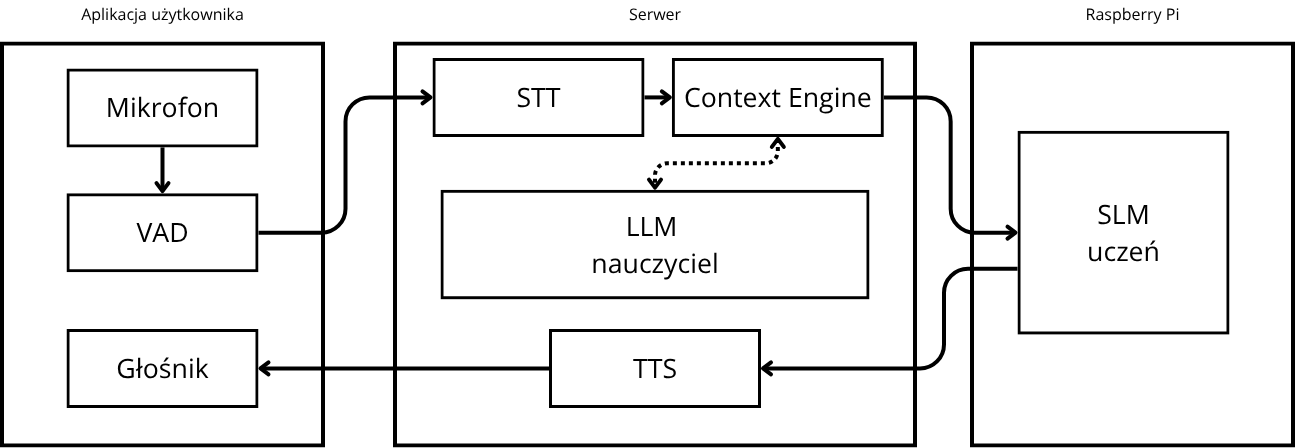
\includegraphics[width=1\linewidth]{src/img/system-schemat.png}
    \caption{Architektura systemu.}
    \label{fig:schemat}
\end{figure}

Przedstawiona architektura zakłada wykorzystanie istniejącej aplikacji użytkownika, rozwijanej wcześniej w ramach systemu Wilga MiLL. W ramach niniejszej pracy nie projektowano aplikacji od podstaw, lecz przyjęto rozszerzenie jej o dodatkową zakładkę asystenta głosowego. Zakładka ta pełni rolę punktu styku pomiędzy użytkownikiem a systemem: umożliwia rozpoczęcie rozmowy, rejestrację wypowiedzi, przekazanie nagrania do dalszego przetwarzania oraz prezentację odpowiedzi w formie tekstowej lub dźwiękowej. Takie podejście pozwala wykorzystać istniejący interfejs, a jednocześnie ogranicza zakres zmian w części aplikacyjnej do funkcji bezpośrednio związanych z asystentem.

W przyjętym rozwiązaniu aplikacja webowa nie realizuje samodzielnie rozpoznawania mowy ani syntezy odpowiedzi. Jej zadaniem jest obsługa interakcji użytkownika oraz przekazanie nagranego sygnału audio do warstwy serwerowej. Po stronie serwera uruchamiane są moduły odpowiedzialne za detekcję aktywności głosowej, transkrypcję mowy na tekst oraz zamianę odpowiedzi tekstowej na dźwięk. Rozdzielenie tych zadań uznano za zasadne, ponieważ pozwala ograniczyć wymagania wobec urządzenia użytkownika oraz skorzystać z większej mocy obliczeniowej dostępnej poza domkiem wypoczynkowym.

Centralnym elementem części badawczej pozostaje mały model językowy, określany jako SLM (Small Language Model), uruchomiony na mikrokomputerze Raspberry Pi. Zdecydowano się wyizolować właśnie ten komponent jako główny element pracujący na sprzęcie o ograniczonych zasobach, ponieważ model językowy stanowi najbardziej wymagającą część całego łańcucha przetwarzania. Raspberry Pi 5 wyposażone w 8 GB pamięci RAM i pozbawione dedykowanej karty graficznej narzuca istotne ograniczenia, dlatego praca koncentruje się na sprawdzeniu, czy pojedynczy lokalny model może generować odpowiedzi o jakości wystarczającej dla użytkownika końcowego.

Drugim modelem w systemie jest większy model językowy, pełniący rolę nauczyciela. Jest on uruchamiany po stronie serwera i odpowiada za przygotowywanie informacji pomocniczych dla modelu ucznia. Jego zadaniem nie jest bezpośrednia obsługa każdej wypowiedzi użytkownika, lecz cykliczna analiza danych oraz tworzenie syntetycznego kontekstu, który może zostać przekazany do małego modelu. Dzięki temu model uruchomiony na Raspberry Pi nie musi samodzielnie analizować pełnych przebiegów czasowych systemu IoT, lecz korzysta z wcześniej przygotowanej reprezentacji wiedzy.

Za koordynację tego procesu odpowiada moduł nazwany Context Engine. W projekcie przyjęto, że jest to zestaw skryptów przygotowanych w języku Python, których zadaniem jest cykliczne pobieranie danych, kierowanie zapytań do modelu nauczyciela oraz budowanie treści wstrzykiwanej następnie do promptu modelu ucznia. Zastosowanie takiego modułu wynika ze sposobu działania modeli językowych, które nie prowadzą samodzielnej, ciągłej analizy środowiska, lecz generują odpowiedź dopiero po otrzymaniu odpowiedniego zapytania. Konieczne było zatem zaprojektowanie warstwy pośredniej, która regularnie przygotowuje kontekst i udostępnia go lokalnemu modelowi w formie możliwej do wykorzystania podczas rozmowy.

Przepływ danych rozpoczyna się od wypowiedzi użytkownika zarejestrowanej w aplikacji webowej. Nagranie jest przekazywane do serwera, gdzie następuje jego przetworzenie do postaci tekstowej. Następnie zapytanie użytkownika zostaje połączone z kontekstem przygotowanym przez Context Engine i przekazane do modelu ucznia uruchomionego na Raspberry Pi. Wygenerowana odpowiedź wraca do warstwy serwerowej, gdzie może zostać przekształcona na mowę, a następnie jest prezentowana użytkownikowi w aplikacji. Taki podział odpowiedzialności pozwala połączyć zalety lokalnej inferencji modelu SLM z możliwościami obliczeniowymi infrastruktury serwerowej.

\newpage
\section{Środowisko projektowo-badawcze}

\subsection{Uzasadnienie wyboru platformy brzegowej}

Jako referencyjną platformę brzegową dla modelu ucznia wybrano mikrokomputer Raspberry Pi 5 w wersji wyposażonej w 8 GB pamięci RAM. Wybór ten wynikał z kilku powiązanych przesłanek projektowych. Po pierwsze, urządzenia tej klasy są powszechnie wykorzystywane w rozwiązaniach Internetu Rzeczy, ponieważ łączą niewielkie rozmiary, umiarkowany pobór energii oraz możliwość pracy jako niezależne węzły systemu. Po drugie, komputery Raspberry Pi były już stosowane w środowisku systemu Wilga MiLL jako elementy odpowiedzialne za agregację danych oraz obsługę wybranych funkcji lokalnych. Z tego względu wykorzystanie tej samej klasy sprzętu pozwala zachować spójność z istniejącą infrastrukturą.

Istotnym kryterium wyboru była również ograniczona moc obliczeniowa tej platformy. Raspberry Pi 5 nie jest wyposażone w dedykowaną kartę graficzną przeznaczoną do przyspieszania obliczeń związanych z inferencją modeli językowych. W konsekwencji uruchamianie modelu LLM lub SLM na takim urządzeniu wymaga dobrania odpowiednio małego modelu, zastosowania kwantyzacji oraz ograniczenia długości kontekstu przekazywanego do promptu. Ograniczenia te uznano za zgodne z celem pracy, ponieważ pozwalają zbadać praktyczne możliwości działania lokalnego asystenta głosowego na sprzęcie o zasobach zbliżonych do urządzeń wykorzystywanych w systemach IoT.

Zastosowanie Raspberry Pi 5 jako platformy odniesienia pozwala również odtworzyć warunki, w których rozwiązanie mogłoby zostać wdrożone w domku wypoczynkowym. Urządzenie może pracować lokalnie, w pobliżu źródeł danych i interfejsu użytkownika, bez konieczności przekazywania każdego zapytania do zewnętrznej usługi chmurowej. Takie podejście wpisuje się w założenia architektury brzegowej, w której część przetwarzania wykonywana jest możliwie blisko miejsca powstawania danych.

\subsection{Architektura sprzętowa}

W projekcie rozważono dwa typy jednostek obliczeniowych. Pierwszą z nich jest urządzenie brzegowe, czyli Raspberry Pi 5, na którym uruchamiany jest model ucznia. Jego zadaniem jest obsługa właściwego zapytania użytkownika połączonego z przygotowanym wcześniej kontekstem. Drugi typ jednostki stanowi platforma serwerowa, przeznaczona do okresowego uruchamiania większego modelu językowego pełniącego rolę nauczyciela. Taki podział odpowiedzialności wynika z architektury opisanej w rozdziale dotyczącym koncepcji systemu i pozwala rozdzielić zadania wymagające szybkiej lokalnej odpowiedzi od zadań wymagających większej mocy obliczeniowej.

Jako jedną z możliwych platform dla modelu nauczyciela rozważono stację roboczą znajdującą się w laboratorium LaVa na Wydziale Elektroniki i Technik Informacyjnych Politechniki Warszawskiej. Komputer ten wyposażony jest w kartę graficzną NVIDIA GeForce RTX 3050, co czyni go odpowiednim kandydatem do uruchamiania większych modeli językowych niż te możliwe do zastosowania na Raspberry Pi. Wykorzystanie takiej jednostki pozwoliłoby przenieść bardziej kosztowne obliczeniowo zadania, takie jak analiza większych zbiorów danych historycznych, poza urządzenie brzegowe.

Alternatywną platformą dla modelu nauczyciela jest komputer MacBook z układem Apple M4 i 16 GB pamięci zunifikowanej. Zaletą tej klasy sprzętu jest architektura Apple Silicon, w której pamięć współdzielona może być wykorzystywana przez różne jednostki obliczeniowe układu. W praktyce ułatwia to uruchamianie lokalnych modeli językowych, szczególnie w porównaniu z klasycznymi konfiguracjami, w których ograniczeniem bywa oddzielna pojemność pamięci karty graficznej. Z tego względu zdecydowano się rozpocząć prace implementacyjne i testy integracyjne od tej platformy, ponieważ była łatwiej dostępna w trakcie realizacji projektu.

Przyjęcie MacBooka jako początkowej platformy dla modelu nauczyciela nie wyklucza wykorzystania stacji roboczej z kartą NVIDIA GeForce RTX 3050 w kolejnych etapach. Zmiana platformy może okazać się zasadna w przypadku testów wymagających porównania czasu generacji, obsługi większego modelu lub stabilniejszego środowiska pracy długotrwałych procesów serwerowych. W ten sposób architektura pozostaje elastyczna, a wybór konkretnej jednostki dla modelu nauczyciela może zostać dostosowany do potrzeb badań.

W przyjętej topologii Raspberry Pi pełni rolę lokalnego węzła uruchomieniowego dla modelu ucznia. Aplikacja użytkownika komunikuje się z warstwą serwerową, która odpowiada za obsługę nagrania, transkrypcję mowy, syntezę odpowiedzi oraz przygotowanie kontekstu. Dane kontekstowe są cyklicznie generowane przez komponent serwerowy i wykorzystywane przy obsłudze zapytań kierowanych do modelu lokalnego. Takie rozdzielenie elementów sprzętowych pozwala ograniczyć obciążenie urządzenia brzegowego, a jednocześnie zachować lokalny charakter inferencji wykonywanej przez model ucznia.

\subsection{Uruchamianie modeli LLM na edge: wyzwania i ograniczenia}

Uruchamianie modeli językowych na urządzeniach brzegowych stanowi istotne wyzwanie techniczne, przede wszystkim ze względu na ograniczoną ilość pamięci operacyjnej oraz brak dedykowanego układu GPU. W przypadku przyjętej platformy referencyjnej dostępne jest 8 GB pamięci RAM, która musi wystarczyć zarówno na system operacyjny, środowisko uruchomieniowe, jak i sam model wraz z kontekstem wejściowym. Oznacza to, że pełnowymiarowe modele LLM, których liczba parametrów może sięgać dziesiątek lub setek miliardów, nie są możliwe do praktycznego wykorzystania w analizowanym środowisku.

Z tego względu w pracy skoncentrowano się na małych modelach językowych klasy SLM. Modele te mają zwykle kilka miliardów parametrów i mogą być uruchamiane lokalnie po zastosowaniu odpowiedniego formatu zapisu oraz kwantyzacji. Zmniejszenie precyzji wag pozwala ograniczyć rozmiar modelu i zapotrzebowanie na pamięć, jednak może również wpływać na jakość generowanych odpowiedzi. Dobór modelu nie może więc opierać się wyłącznie na jego rozmiarze, lecz powinien uwzględniać kompromis pomiędzy jakością odpowiedzi, czasem generacji oraz stabilnością działania na platformie brzegowej.

Szczególne znaczenie ma opóźnienie odpowiedzi. W przypadku asystenta głosowego użytkownik oczekuje reakcji w czasie zbliżonym do naturalnej rozmowy, dlatego zbyt długie oczekiwanie na pierwszy token lub zakończenie wypowiedzi może obniżyć użyteczność całego rozwiązania. Jednocześnie zwiększanie rozmiaru modelu lub długości kontekstu zwykle prowadzi do wzrostu zużycia pamięci oraz wydłużenia czasu inferencji. W związku z tym w dalszej części pracy analizie poddano nie tylko wybór konkretnego modelu, lecz także parametry generacji i sposób przygotowania promptu.

Ograniczenia środowiska edge wpłynęły również na decyzję o zastosowaniu architektury Nauczyciel-Uczeń. Model lokalny nie powinien samodzielnie analizować pełnych zbiorów danych historycznych, ponieważ wymagałoby to przekazania długiego kontekstu i zwiększyłoby czas odpowiedzi. Zamiast tego założono, że bardziej zasobożerny model nauczyciela przygotowuje syntetyczne podsumowania, które następnie są wykorzystywane przez model ucznia. Takie podejście pozwala zmniejszyć ilość danych przetwarzanych bezpośrednio na Raspberry Pi, a jednocześnie zachować możliwość udzielania odpowiedzi powiązanych z rzeczywistym stanem systemu IoT.

\subsection{Wykorzystane oprogramowanie i technologie}

\subsubsection{Aplikacja użytkownika}

Aplikacja użytkownika nie była tworzona w ramach pracy od podstaw. Zdecydowano się rozszerzyć istniejącą aplikację systemu Wilga MiLL o funkcje związane z asystentem głosowym, ponieważ pozwala to wykorzystać już przygotowany interfejs oraz mechanizmy komunikacji z systemem. W konsekwencji podstawowy stos technologiczny części frontendowej został narzucony przez istniejące rozwiązanie.

Aplikacja została przygotowana z wykorzystaniem biblioteki React, języka TypeScript oraz narzędzia Vite. Komunikacja z warstwą serwerową odbywa się z użyciem protokołu HTTP oraz połączeń WebSocket. Taki zestaw technologii umożliwia zarówno obsługę klasycznych żądań, jak i przekazywanie informacji aktualizowanych w czasie rzeczywistym. W kontekście projektowanego asystenta szczególne znaczenie ma możliwość sprawnego przekazywania nagrań, odbierania wyników przetwarzania oraz prezentowania odpowiedzi użytkownikowi w aplikacji.

\subsubsection{Warstwa serwerowa i komunikacyjna}

Warstwa serwerowa pełni funkcję pośrednią pomiędzy aplikacją użytkownika, modułami przetwarzania mowy, modelem nauczyciela oraz modelem ucznia. Do jej implementacji przyjęto język Python, ponieważ jest on szeroko wykorzystywany w rozwiązaniach związanych z uczeniem maszynowym i umożliwia wygodną integrację z bibliotekami obsługującymi modele językowe oraz przetwarzanie dźwięku. Jako technologię budowy interfejsu API wskazano FastAPI, które pozwala tworzyć lekkie usługi HTTP oraz endpointy wykorzystywane przez aplikację frontendową.

Zastosowanie osobnej warstwy serwerowej ułatwia rozdzielenie odpowiedzialności poszczególnych komponentów. Aplikacja webowa odpowiada za interakcję z użytkownikiem, natomiast serwer koordynuje przepływ danych, uruchamia moduły przetwarzania mowy i przekazuje zapytania do odpowiednich modeli. Takie podejście ogranicza złożoność części frontendowej oraz pozwala testować poszczególne elementy systemu niezależnie.

\subsubsection{Moduły STT i TTS}

Obsługa interfejsu głosowego wymaga zastosowania modułów odpowiedzialnych za rozpoznawanie mowy oraz syntezę odpowiedzi. W projekcie założono wykorzystanie gotowych rozwiązań, ponieważ główny zakres pracy dotyczy architektury współpracy modeli językowych oraz działania małego modelu na platformie brzegowej. Samodzielna implementacja algorytmów STT i TTS znacząco rozszerzyłaby zakres projektu, nie stanowiąc jednocześnie głównego problemu badawczego.

Do rozpoznawania mowy przewidziano wykorzystanie rozwiązania zgodnego z modelem Whisper, w szczególności implementacji typu faster-whisper, która pozwala uruchamiać transkrypcję w sposób bardziej dostosowany do lokalnych zasobów obliczeniowych. Zadaniem tego modułu jest przekształcenie nagrania użytkownika do postaci tekstowej, która może zostać następnie przekazana do modelu językowego. Synteza mowy pełni funkcję odwrotną i umożliwia przedstawienie odpowiedzi modelu w formie dźwiękowej. W obu przypadkach kluczowe znaczenie mają opóźnienie oraz poprawność działania w języku polskim.

\subsubsection{LLM}

Do uruchamiania modeli językowych wykorzystano środowisko Ollama. Narzędzie to umożliwia lokalne uruchamianie modeli LLM i SLM oraz udostępnianie ich przez interfejs API, co ułatwia integrację z pozostałymi komponentami systemu. Zastosowanie jednego środowiska uruchomieniowego dla modelu ucznia i modelu nauczyciela pozwala ograniczyć liczbę różnic konfiguracyjnych pomiędzy platformami oraz uprościć przebieg testów.

Istotną zaletą wykorzystania Ollama jest możliwość uruchamiania modeli z określonymi parametrami generacji. Parametry takie jak temperatura, długość odpowiedzi, liczba przetwarzanych tokenów kontekstu czy sposób próbkowania mogą wpływać zarówno na jakość odpowiedzi, jak i na czas jej wygenerowania. Z tego względu środowisko to uznano za odpowiednie do prowadzenia badań porównawczych, w których analizowany jest wpływ konfiguracji modelu na działanie asystenta.

\subsubsection{Serwerowy Context Engine}

W celu dynamicznego dostarczania kontekstu do małego modelu językowego zaprojektowano komponent określany jako Context Engine. Jego zadaniem jest cykliczne pobieranie danych, kierowanie zapytań do modelu nauczyciela oraz przygotowywanie syntetycznych podsumowań, które mogą zostać dołączone do promptu modelu ucznia. Zastosowanie takiego komponentu wynika z ograniczeń platformy brzegowej oraz z potrzeby ograniczenia długości kontekstu analizowanego bezpośrednio przez Raspberry Pi.

Context Engine zaimplementowano jako zestaw skryptów w języku Python. Skrypty te mogą być uruchamiane cyklicznie, dzięki czemu kontekst przekazywany do modelu ucznia jest aktualizowany niezależnie od bieżącej rozmowy użytkownika. W momencie obsługi zapytania przygotowany wcześniej kontekst może zostać wstrzyknięty do promptu, co pozwala modelowi lokalnemu korzystać z informacji o stanie systemu bez konieczności samodzielnej analizy pełnych danych historycznych. Takie rozwiązanie ogranicza obciążenie urządzenia brzegowego i zwiększa przewidywalność czasu odpowiedzi.

\subsubsection{Narzędzia badawcze}

Część badawcza wymagała przygotowania środowiska umożliwiającego porównywanie modeli oraz konfiguracji generacji. Z tego względu przewidziano wykorzystanie skryptów testowych w języku Python, które pozwalają automatyzować uruchamianie zapytań, zapisywanie wyników oraz analizę podstawowych metryk. W procesie optymalizacji parametrów można wykorzystać narzędzie Optuna, które wspiera systematyczne przeszukiwanie przestrzeni parametrów i ułatwia porównywanie wielu konfiguracji.

Tak przygotowane środowisko pozwala oddzielić ocenę jakości odpowiedzi od ręcznego uruchamiania pojedynczych testów. Ma to znaczenie szczególnie w przypadku modeli działających na urządzeniu brzegowym, gdzie czas generacji może być zmienny i zależny od obciążenia systemu, długości promptu oraz wybranych parametrów. Automatyzacja testów zwiększa powtarzalność badań i ułatwia późniejsze zestawienie wyników w części badawczej pracy.

% ============================================================
%  ROZDZIAŁ: Część badawcza
% ============================================================

\newpage
\graphicspath{{data/5 - badania/wykresy/}}
\section{Część badawcza: analiza porównawcza i optymalizacja SLM na urządzeniu brzegowym}
\label{sec:modele}

Część badawcza stanowi zasadniczy punkt niniejszej pracy magisterskiej.
Jej celem było empiryczne sprawdzenie, na ile mały model językowy może
działać użytecznie na urządzeniu brzegowym o~bardzo ograniczonych zasobach.
Raspberry~Pi~5 z~8~GB pamięci RAM, bez dedykowanego GPU, wymusza kompromisy
między jakością odpowiedzi, opóźnieniem oraz stabilnością inferencji; bez
systematycznych pomiarów trudno byłoby uzasadnić wybór modelu, kwantyzacji
czy konfiguracji generacji w~takim środowisku.

W~rozdziale zbadano m.in.\ wpływ hiperparametrów Ollamy, wariantów kwantyzacji
GGUF oraz warunków pomiaru (w~tym stanów \emph{cold} i~\emph{warm cache})
na metryki jakościowe i~wydajnościowe lokalnego SLM. Choć eksperymenty
przeprowadzono w~kontekście asystenta głosowego systemu Wilga~MiLL, uzyskane
wnioski mają charakter ogólniejszy: dotyczą uruchamiania małych modeli
językowych na typowym sprzęcie IoT i~mogą być wykorzystane także w~innych
aplikacjach brzegowych o~podobnych ograniczeniach pamięci i~mocy obliczeniowej.

% ============================================================
\subsection{Architektura i metodologia systemu benchmarkowego}
\label{subsec:metodologia}
% ============================================================

\subsubsection{Komponenty systemu testowego}

Założeniem dla budowy systemu testowego nie było uruchamianie pełnego produkcyjnego pipeline'u aplikacji Wilga, lecz
stworzenie wycinka systemy, który pozwoli poddać testom modele SLM na urządzeniu brzegowym. Architektura systemu pomiarowego składa
się z~dwóch bloków: serwera orkiestrującego (MacBook) oraz
platformy brzegowej (Raspberry~Pi~5), przedstawionych na
rysunku~\ref{fig:testy_arch}.

Po stronie serwera pracuje skrypt \texttt{tester.py}, który pełni rolę orchestratora. Dla
każdego przypadku z~\texttt{golden.jsonl} pobiera \emph{system\_prompt},
łączy go z~pytaniem użytkownika i~wysyła żądanie HTTP do Ollamy uruchomionej
na Raspberry~Pi. Po stronie serwera mierzone są parametry czasowe: TTFT(time to first token) oraz E2E(end to end). Po otrzymaniu odpowiedzi modelu
orkiestrator przekazuje ją do modelu zewnętrznego oceniającego jakość odpowiedzi. Ponownie korzystając z OpenRouter podłączono się do modelu Claude, tym razem był to Haiku 3.5. Zastosowano mniejszy, tańszy model, gdyż benchmark wymagał wysyłania wielu żądań, a koszty największych modeli są wygórowane. Haiku zwracał pięć metryk jakościowych, opisanych w~tabeli~\ref{tab:haiku_metryki}.

Prompt przekazywany do Haiku składał się z~czterech elementów wejściowych:
\begin{equation}
  \label{eq:haiku_prompt}
  \mathrm{prompt}_{\mathrm{Haiku}}
  =
  \{\mathrm{system\_prompt}\}
  +
  \{\mathrm{question}\}
  +
  \{\mathrm{golden\_answer}\}
  +
  \{\mathrm{model\_answer}\},
\end{equation}
\noindent
gdzie \emph{system\_prompt} to kontekst stanu domu zbudowany wcześniej
z rzeczywistych wierszy danych sensorowych, \emph{question} to pytanie użytkownika, \emph{golden\_answer}
odpowiedź wzorcowa, natomiast \emph{model\_answer} to odpowiedź badanego SLM.
W~prompcie wskazano ponadto, że kontekst sensorowy jest jedynym źródłem
prawdy, a~wynik musi zostać zwrócić jako JSON z~pięcioma metrykami. Flaga halucynacji miała być ustawiana tylko wtedy, gdy model
podaje konkretne fakty spoza kontekstu. Temperaturę ewaluacji ustawiono
na zero, żeby oceny były możliwie powtarzalne. Otrzymana odpowiedź była przetwarzna oraz odrzucana jeśli format nie odpowiadał żądanemu JSON. Wymuszenie pozostaje jednak miękkie, w przypadku dalszej ewaluacji testów za istotne uznano zastosowanie mechanizmów takich jak \href{https://ai.pydantic.dev/output/}{Pydantic AI} czy \href{https://docs.langchain.com/oss/python/langchain/structured-output}{LangChain} pozwalających deterministycznie definiować format odpowiedzi modeli językowych.

Na urządzeniu brzegowym Raspberry Pi 5 działa serwer Ollamy, który dzięki funkcji API pozwala na łatwe odpytywanie wielu modeli zainstalowanych na urządzeniu. Eównolegle działał również mikroserwer \texttt{metrics\_server.py}, jego wprowadzenie było konieczne aby mierzyć temperaturę CPU, zużycie RAM oraz flagę dławienia (throttling flag, przegrzanie procesora).

\begin{figure}[H]
  \centering
  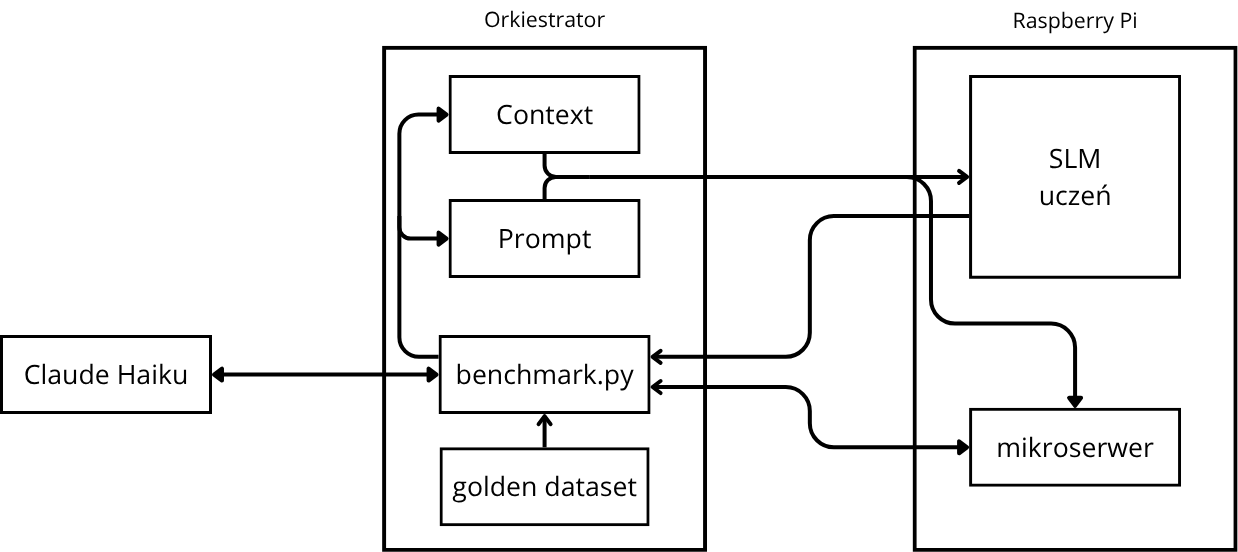
\includegraphics[width=0.85\textwidth]{src/img/testy-schemat.png}
  \caption{Schemat systemu benchmarkowego. Serwer (MacBook~M4) pełni rolę
           orchestratora i~hosta ewaluatora; Raspberry~Pi~5 jest platformą
           inferencji.}
  \label{fig:testy_arch}
\end{figure}

\subsubsection{Zbiór danych testowych}


Pracę nad częścią badawczą rozpoczęto od zbiory zawierającego pytania oraz modelowe odpowiedzi. Jest nim plik \texttt{golden.jsonl}: stały zbiór 20~przypadków testowych. Każdy rekord zawiera identyfikator
przypadku, jego kategorię, tekstowy \emph{system\_prompt} zbudowany z~realnego
wiersza danych sensorowych, pytanie użytkownika oraz
wzorcową odpowiedź \emph{golden\_answer}. Zbiór wygenerowano jednorazowo przy użyciu modelu Claude Sonnet~4.6. Wybór modelu znacznie większego i~bardziej zaawansowanego od lokalnie uruchamianych modeli (omawianych w pracy) pozwolił zapewnić wysoką jakość odpowiedzi referencyjnych. Do integracji i~wywołania modelu wykorzystano API platformy \href{https://openrouter.ai}{OpenRouter}, będącej wygodnym agregatorem modeli językowych od wielu dostawców.

Rozkład kategorii przypadków przedstawiono w~tabeli~\ref{tab:golden_kategorie}.

\begin{table}[H]
  \centering
  \caption{Kategorie przypadków w~złotym zbiorze testowym (20~przypadków).}
  \label{tab:golden_kategorie}
  \begin{tabular}{lrl}
    \hline
    Kategoria & Liczba & Co testuje \\
    \hline
    \texttt{factual\_status}   & 8 & Poprawne odczytanie stanu z~kontekstu \\
    \texttt{missing\_data}     & 4 & Przyznanie braku danych zamiast zgadywania \\
    \texttt{conflicting\_data} & 3 & Wykrycie sprzeczności w~danych \\
    \texttt{stale\_data}       & 2 & Sygnalizacja nieaktualności odczytu \\
    \texttt{paraphrase}        & 3 & Spójność odpowiedzi na te same pytania \\
    \hline
    \textbf{Razem}             & \textbf{20} & \\
    \hline
  \end{tabular}
\end{table}

Kategorie \texttt{missing\_data} i~\texttt{stale\_data} uznano za najbardziej wymagające,
ponieważ są podatne na halucynacje, która jak zaznaczono w analizie literatury \ref{sec:analiza_literatury} jest krytycznym czynnikiem w ocenie jakości odpowiedzi modeli językowych.

\subsubsection{Metryki oceny i wzór composite score}
\label{subsec:metryki}

\begin{table}[H]
  \centering
  \caption{Metryki oceny stosowane w~benchmarku (trzy grupy).}
  \label{tab:haiku_metryki}
  \begin{tabular}{cllp{5.6cm}}
    \hline
    Grupa & Metryka & Zakres & Znaczenie \\
    \hline
    1 & TTFT & ms & Czas do pierwszego tokenu \\
    1 & E2E & ms & Czas do ostatniego tokenu \\
    1 & \emph{generation\_ms} & ms & $\mathrm{E2E}-\mathrm{TTFT}$ \\
    1 & RAM & MB & Zużycie pamięci na Raspberry~Pi \\
    1 & temperatura CPU & $^\circ$C & Temperatura procesora z~mikroserwera \\
    1 & flaga dławienia & binarna & Przegrzanie / throttling procesora \\
    \hline
    2 & \texttt{faithfulness} & $[0,1]$ & Czy każde twierdzenie faktyczne wynika z~kontekstu sensorowego \\
    2 & \texttt{answer\_relevancy} & $[0,1]$ & Czy odpowiedź adresuje zadane pytanie \\
    2 & \texttt{conciseness} & $[0,1]$ & Czy odpowiedź jest zwięzła, bez zbędnych informacji \\
    2 & \texttt{hallucination\_flag} & binarna & \texttt{true}, gdy odpowiedź zawiera fakty spoza kontekstu; zeruje wynik łączny \\
    \hline
    3 & \texttt{polish\_quality} & $[0,1]$ & Naturalność i~poprawność języka polskiego; rejestrowana, poza \emph{composite score} \\
    \hline
  \end{tabular}
\end{table}

Metryki z~tabeli~\ref{tab:haiku_metryki} podzielono na trzy grupy.
Grupa~1 obejmuje metryki wydajnościowe mierzone deterministycznie przez urządzenie brzegowe.
Grupa~2 to metryki jakościowe zwracane przez LLM-oceniający (Haiku~3.5).
Grupa~3 obejmuje \emph{polish\_quality} został dodany w celu przyszłych ewaluacji jakościowych odpowiedzi.

Metryki z grupy drugiej składają się na \emph{composite score}. W oparciu o literaturę oraz standardy \cite{Es2024Ragas,ConCISE2025,DefAn2024} przyjęto go jako sposób matematycznego wyznaczania jakości odpowiedzi porównywanych modeli. Konieczne 
do wyznaczenia composite score było przyjęcie wag dla każdej z metryk. Wzór przedstawiony w równaniu \ref{eq:composite_score}.

\begin{equation}
  \label{eq:composite_score}
  \mathrm{score} =
  \begin{cases}
    0{,}0 & \text{gdy } \mathrm{hallucination\_flag} = \mathrm{true} \\[6pt]
    0{,}40 \cdot f + 0{,}30 \cdot r + 0{,}20 \cdot c + \ell & \text{w~przeciwnym razie}
  \end{cases}
\end{equation}
\noindent
gdzie $f$, $r$, $c$ to odpowiednio \emph{faithfulness}, \emph{answer\_relevancy}
i~\emph{conciseness}, a~$\ell = 0{,}05 \cdot (1 - \min(\mathrm{e2e\_ms}/90\,000,\, 1))
+ 0{,}05 \cdot (1 - \min(\mathrm{ttft\_ms}/45\,000,\, 1))$.

W prezenotwanym rozwiązaniu\emph{faithfulness} ma najwyższą wagę, ponieważ odpowiedź trzymająca się faktów jest niezwykle istotna w konktekście tej pracy- asystenta głoswoego. Składniki opóźnienia (E2E
i~TTFT, łącznie 0{,}10) zostały rozdzielone, ponieważ moduł TTS może rozpocząć
syntezę mowy przed zakończeniem generacji tokenów co powoduje wrażenie bardziej płynnej interakcji. 

\subsubsection{Dostrajanie parametrów pracy modelu}

Optymalizację hiperparametrów inferencji modelu przeprowadzono z wykorzystaniem biblioteki Optuna
wykorzystującej metodę TPE (\emph{Tree-structured Parzen Estimator}). Przeszukiwana
przestrzeń współczynnik pracy modelu przedstawiono w~tabeli~\ref{tab:optuna_hparams}.

\begin{table}[H]
  \centering
  \caption{Przestrzeń hiperparametrów przeszukiwana przez Optunę (TPE).}
  \label{tab:optuna_hparams}
  \begin{tabular}{lll}
    \hline
    Parametr & Typ & Zakres \\
    \hline
    \texttt{temperature}    & float       & $[0{,}10,\; 0{,}80]$ \\
    \texttt{num\_ctx}       & categorical & $\{1024,\; 2048,\; 4096\}$ \\
    \texttt{num\_predict}   & int         & $[48,\; 160]$ \\
    \texttt{top\_p}         & float       & $[0{,}80,\; 0{,}99]$ \\
    \texttt{repeat\_penalty}& float       & $[1{,}00,\; 1{,}15]$ \\
    \hline
  \end{tabular}
\end{table}

Pełna siatka parametrów wynosi $8 \times 3 \times 3 \times 5 \times 4
= 1440$ kombinacji $\times$ 20~promptów $= 28\,800$ zapytań. Optuna z~80~trialami (przejściami przez pełny zestaw 20 pytań)
($80 \times 20 = 1600$ ewaluacji LLM-oceniającego) osiąga porównywalne pokrycie
obszarów obiecujących dzięki istocie swojego działania. Nie prowadzono testów Nie na wszystkich modelach przeprowadzano testy tej samej długości.

\subsubsection{Modele kandydujące}

Do badań wybrano sześć modeli klasy SLM, których wielkość zawierała się w przedziale  2--5B parametrów. Kierowano się przede wszystim wielkością modelu oraz postanowiono postawić na znanych dostawców. Tabela~\ref{tab:modele_kandydaci}
przedstawia wybranych kandydatów..

\begin{table}[H]
  \centering
  \caption{Modele kandydujące i~ich udział w~benchmarku Optuny.}
  \label{tab:modele_kandydaci}
  \small
  \begin{tabular}{lllll}
    \hline
    Model & Parametry & GGUF Q4\_K\_M & Producent \\
    \hline
    Llama~3.2~3B  & 3{,}2~mld & ${\sim}$2{,}0~GB & Meta        \\
    Phi-3.5 Mini  & 3{,}8~mld & ${\sim}$2{,}4~GB & Microsoft  \\
    Gemma~2~2B    & 2{,}6~mld & ${\sim}$1{,}7~GB & Google     \\
    Gemma~3~4B    & 4{,}0~mld & ${\sim}$2{,}3~GB & Google     \\
    Qwen~2.5~3B   & 3{,}0~mld & ${\sim}$2{,}0~GB & Alibaba    \\
    Bielik~4.5B   & 4{,}5~mld & ${\sim}$2{,}7~GB & SpeakLeash \\
    \hline
  \end{tabular}
\end{table}


% ============================================================
\subsection{Etap Optuna: chłodzenie, hiperparametry i dominacja halucynacji}
\label{subsec:optuna}
% ============================================================

\subsubsection{Warunek termiczny pomiaru}
\label{subsec:run1}
\label{subsec:run2}

Testy rozpoczęto ze wskazaną wyżej grupą modeli. Bardzo szybko okazało się, że czsy odpowiedzi bardzo często przekraczają górną granicę pomiaru, którą wyznaczono na 60 sekund. Po analizie danych jasna stała się przyczyna.
W~każdym z~500~rekordów procesor pracował
w~trybie throttling (ang. dławienie). Dzięki pomiarom mikroserwera na RPi możliwe było odczytanie temperatury CPU.
Na Raspberry~Pi~5 throttling jest metodą ograniczania częstotliwości taktowania procesora w celu obniżenia temperatury, skutkuje ona znacznym obniżeniem mocy obliczeniowej jednostki. Pierwsze ogaraniczenia aktywowane są przy ~80\,°C, a~twarde
dławienie (\texttt{vcgencmd get\_throttled 0x2}) ok.~85\,°C.

Przy przekroczeniu limitu czasu (60\,s) Ollama zwraca pustą odpowiedź, którą
LLM-judge klasyfikuje jako halucynację (score $= 0$). Odnotowano 169~timeoutów
z~korelacją 100\% względem flagi halucynacji. Dla \texttt{gemma3:4b} 42\%
rekordów kończyło się timeoutem. W~efekcie ranking z~tabeli~\ref{tab:ranking_run1}
był w~zasadzie fałszywy: \texttt{gemma2:2b} zajmował pierwsze miejsce, a~lepszy
semantycznie \texttt{gemma3:4b} spadał na czwarte --- większe modele dłużej
obciążają CPU i~przy braku chłodzenia generują timeouty. Temperatura CPU
utrzymywała się w~zakresie 84{,}0--91{,}7\,°C (mediana 88{,}9\,°C), a~throttling
występował w~100\% przypadków.

\begin{table}[H]
  \centering
  \caption{Ranking modeli bez aktywnego chłodzenia
           ($n=100$ pomiarów na model).}
  \label{tab:ranking_run1}
  \begin{tabular}{clccccc}
    \hline
    \# & Model & Score & Halucynacje & E2E med. [ms] & Mediana temp. [$^\circ$C] & Throttling \\
    \hline
    1 & \texttt{gemma2:2b}  & 0{,}693 & 16\% & 37\,229 & 87{,}8 & 100\% \\
    2 & \texttt{llama3.2:3b}& 0{,}589 & 30\% & 49\,199 & 88{,}4 & 100\% \\
    3 & \texttt{qwen2.5:3b} & 0{,}547 & 37\% & 53\,169 & 88{,}9 & 100\% \\
    4 & \texttt{gemma3:4b}  & 0{,}497 & 42\% & 57\,584 & 89{,}8 & 100\% \\
    5 & \texttt{phi3.5}     & 0{,}024 & 96\% & 60\,000 & 90{,}0 & 100\% \\
    \hline
  \end{tabular}
\end{table}

Jako receptę na problemy termiczne wskazano aktywne chłodzenie procesora. Układ RPi został rozbudowany o radiator producenta wyposażony w wentylator. Po instalacji chłodzenia przeprowadzono test sprawdzający czy przyniosło ono zamierony efekt. Flaga throttlingu nie została oznaczona w żadnym z przypadków testowych (0/500), a~temperatura CPU do 57{,}6--73{,}6\,°C (mediana 65{,}3\,°C). Zmiana wprowadziła też pierwsze niezerowe wyniki \emph{composite\_score} modeli. Wyniki przedstawiono w tabeli \ref{tab:ranking_run2}.

\begin{table}[H]
  \centering
  \caption{Ranking modeli po zastosowaniu aktywnego chłodzenia.}
  \label{tab:ranking_run2}
  \begin{tabular}{clcccc}
    \hline
    \# & Model & Score & Halucynacje & E2E med. [ms] & Throttling \\
    \hline
    1 & \texttt{gemma3:4b}  & 0{,}806 & 4\%  & 31\,742 & 0\% \\
    2 & \texttt{gemma2:2b}  & 0{,}679 & 19\% & 20\,879 & 0\% \\
    3 & \texttt{qwen2.5:3b} & 0{,}667 & 19\% & 29\,713 & 0\% \\
    4 & \texttt{llama3.2:3b}& 0{,}653 & 20\% & 27\,145 & 0\% \\
    5 & \texttt{phi3.5}     & 0{,}380 & 49\% & 52\,363 & 0\% \\
    \hline
  \end{tabular}
\end{table}

Wstępne problemy z~regulacją termiczną CPU uwydatniły
uwydatnić, jak bardzo stabilność temperaturowa warunkuje
ewaluację modeli językowych na urządzeniach klasy Raspberry Pi 5. Nie spotkało się to ze zdziwieniem, gdyż zagadnienie to szeroko opisaywane jest w literaturze \cite{Tummalapalli2026} oraz przez inżynierów w internecie. Aktywne chłodzenie okazało się zapewniać stabilne warunki pracy platformy i~umożliwiło rzetelne przeprowadzenie dalszych badań.

\subsubsection{Dominacja flagi halucynacji}
\label{subsec:hallucination_dominance}

Pełny przebieg Optuny (\texttt{dataset=results-selected-9.05}, 80~triali)
umożliwił analizę źródeł wariancji \emph{composite score}. Regresja
wieloczynnikowa (rysunek~\ref{fig:regression_r2}) wykazała, że sama flaga
halucynacji wyjaśnia $R^2 = 0{,}9922$ wariancji score --- hiperparametry
inferencji wyjaśniają jedynie $R^2 = 0{,}2997$. Model (\texttt{model\_only})
daje $R^2 = 0{,}8201$; dodanie hiperparametrów (\texttt{model\_plus\_hparams})
podnosi $R^2$ do 0{,}8587 ($\Delta R^2 = 0{,}039$). Pełny model osiąga
$R^2 = 0{,}9982$.

\begin{figure}[H]
  \centering
  
\includegraphics[width=0.85\textwidth]{02_score_vs_hallucination_selected.png}
  \caption{Zależność \emph{composite score} od wskaźnika halucynacji
           (\texttt{results-selected-9.05}). Flaga halucynacji determinuje
           score w~ponad 99\% przypadków.}
  \label{fig:score_vs_hall}
\end{figure}

\begin{figure}[H]
  \centering
  
\includegraphics[width=0.75\textwidth]{07_regression_r2_comparison_selected.png}
  \caption{Porównanie $R^2$ modeli regresji wyjaśniających wariancję score
           (\texttt{results-selected-9.05}).}
  \label{fig:regression_r2}
\end{figure}

Algebraiczna tożsamość $\mathrm{score\_mean} \approx (1 - \mathrm{hall\_rate})
\times \mathrm{nonhall\_score\_mean}$ zachodzi z~błędem poniżej $10^{-8}$.
Rozpiętość \emph{score\_mean} wynosi 0{,}604, podczas gdy rozpiętość
\emph{nonhall\_score} to zaledwie 0{,}119 --- pięciokrotnie mniejsza
(rysunek~\ref{fig:nonhall_spread}).

\begin{figure}[H]
  \centering
  
\includegraphics[width=0.85\textwidth]{03_nonhall_score_spread_selected.png}
  \caption{Rozpiętość \emph{nonhall\_score} w~porównaniu z~\emph{composite score}
           (\texttt{results-selected-9.05}). Hiperparametry nie różnicują
           jakości odpowiedzi bez halucynacji.}
  \label{fig:nonhall_spread}
\end{figure}

Halucynacje koncentrują się w~kategoriach \texttt{missing\_data}
(39{,}4\%) i~\texttt{stale\_data} (29{,}4\%); w~\texttt{factual\_status}
i~\texttt{paraphrase} są marginalne (rysunek~\ref{fig:case_hall_rates}).
Mapa korelacji hiperparametrów (rysunek~\ref{fig:hparam_heatmap}) nie wskazuje
silnych związków z~jakością.

\begin{figure}[H]
  \centering
  
\includegraphics[width=0.85\textwidth]{05_case_hallucination_rates_selected.png}
  \caption{Wskaźnik halucynacji per przypadek testowy
           (\texttt{results-selected-9.05}).}
  \label{fig:case_hall_rates}
\end{figure}

\begin{figure}[H]
  \centering
  
\includegraphics[width=0.75\textwidth]{06_hparam_correlation_heatmap_selected.png}
  \caption{Mapa korelacji hiperparametrów z~metrykami wynikowymi
           (\texttt{results-selected-9.05}). Brak silnych korelacji z~jakością.}
  \label{fig:hparam_heatmap}
\end{figure}

Kluczowy wniosek etapu Optuny: zmiana hiperparametrów wpływa głównie na
\emph{kiedy} model halucynuje, nie na \emph{jak dobrze} odpowiada, gdy nie
halucynuje. Dalsza optymalizacja TPE ma marginalny wpływ na jakość semantyczną.
Problemem są trudne scenariusze wymagające działania na poziomie wag modelu.
To motywuje przejście do kwantyzacji i~\emph{prefix caching} jako dźwigni
opóźnienia oraz plan fine-tuningu (sekcja~\ref{subsec:finetuning_plan}).

\subsubsection{Modelowanie E2E: rozkład normalny}

Dla opóźnienia E2E w~protokole Optuny (zmienny prompt, cold start) przyjęto
model normalny. Rysunek~\ref{fig:optuna_gauss_fit} pokazuje histogramy E2E
oraz dopasowaną gęstość~$\mathcal{N}(\hat\mu,\hat\sigma^2)$ per model.
Lokalizację raportuje się więc jako \textbf{średnią}, a~rozrzut jako~$\sigma$
(nie medianę empiryczną).

\begin{figure}[H]
  \centering
  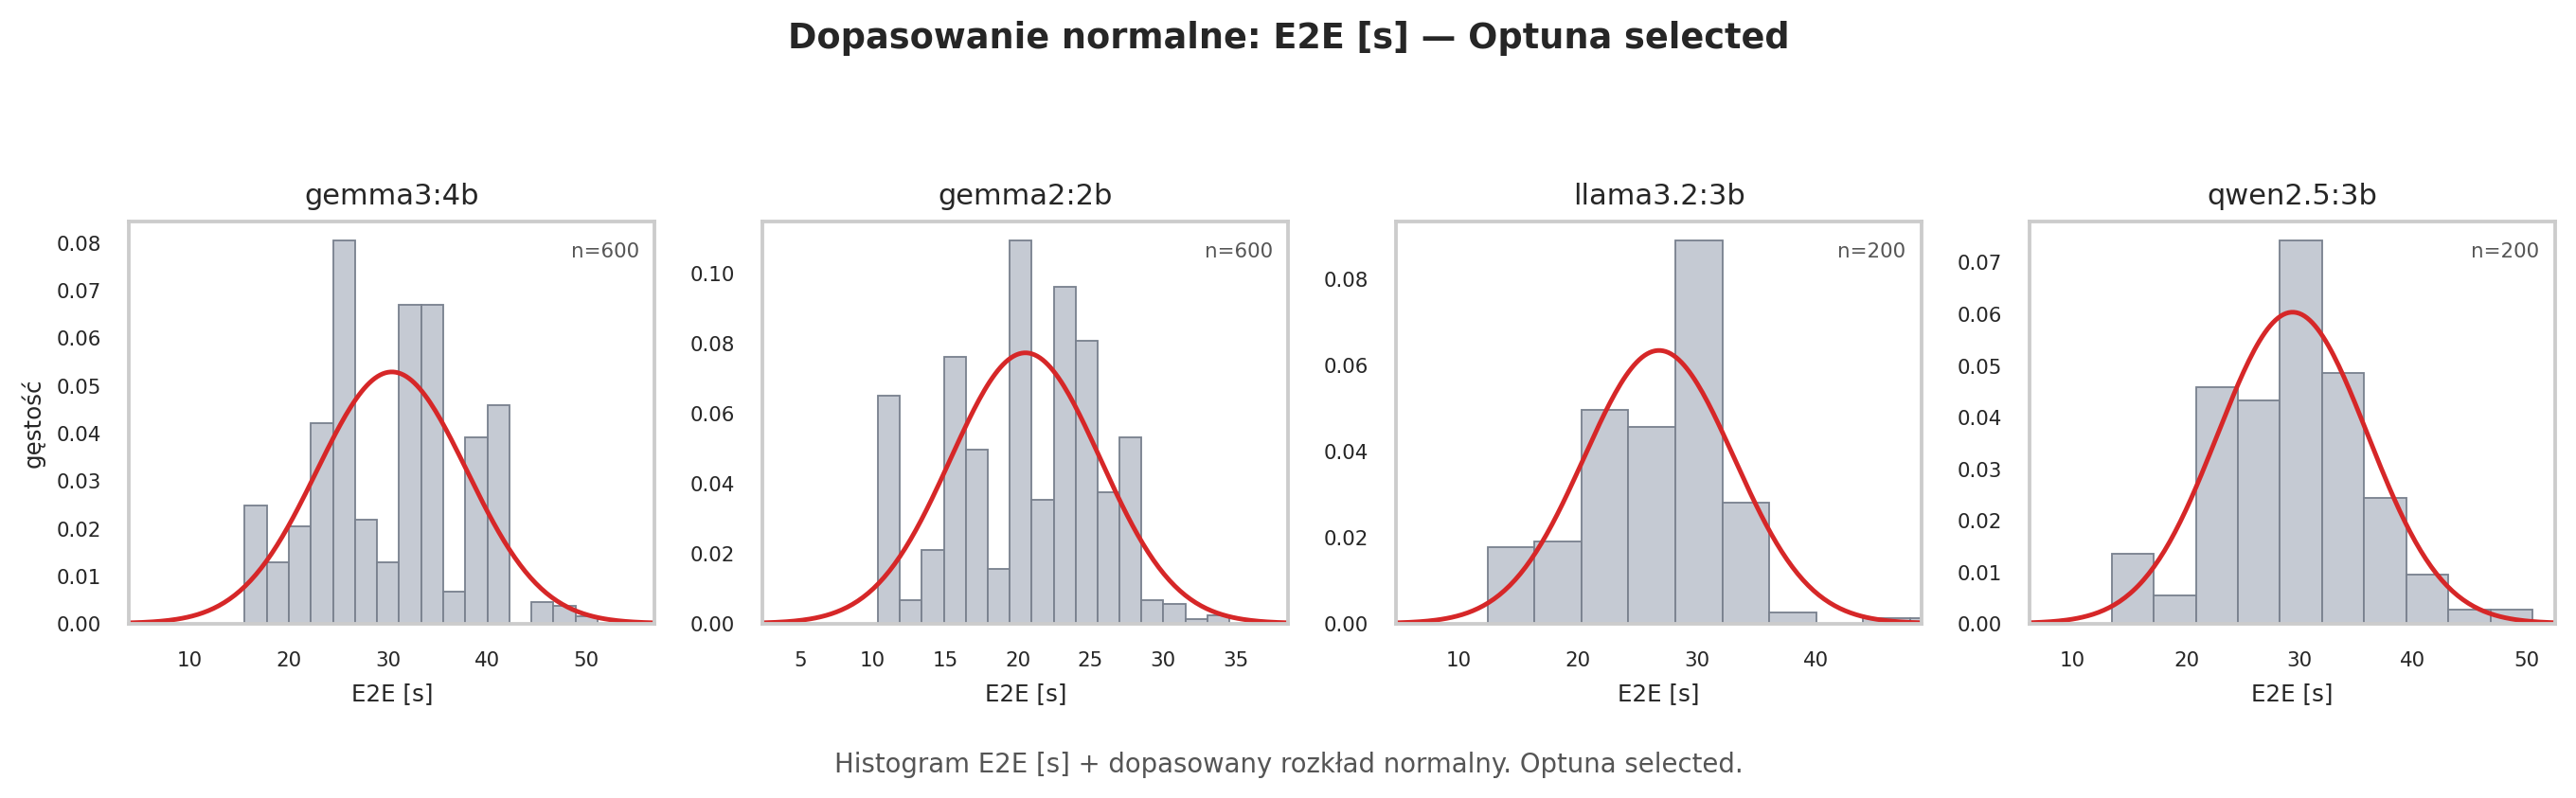
\includegraphics[width=0.95\textwidth]{optuna_e2e_gauss_fit_matrix.png}
  \caption{Dopasowanie rozkładu normalnego do opóźnienia E2E
           (\texttt{results-selected-9.05}). Histogram oraz gęstość
           $\mathcal{N}(\hat\mu,\hat\sigma^2)$ per model.}
  \label{fig:optuna_gauss_fit}
\end{figure}

Kompromis Pareto (rysunek~\ref{fig:pareto_latency_hall}) zestawia średnie E2E
($\pm\sigma$) ze wskaźnikiem halucynacji. Żaden model nie dominuje w~obu
wymiarach jednocześnie: \texttt{gemma2:2b} jest najszybszy
($\mathrm{E2E}\approx 20{,}5$~s), lecz ma ok.~18\%~halucynacji;
\texttt{gemma3:4b} jest wolniejszy ($\approx 30{,}4$~s), lecz osiąga
ok.~1{,}2\%~halucynacji. Dla asystenta informującego o~stanie domu błędna
informacja jest groźniejsza niż kilka sekund dłuższej odpowiedzi --- stąd
wybór \texttt{gemma3:4b} jako kandydata produkcyjnego. Rozsądny preset
hiperparametrów wystarcza; Optuna nie wskazuje silnie dominującej konfiguracji
jakościowej.

\begin{figure}[H]
  \centering
  
\includegraphics[width=0.85\textwidth]{04_latency_hallucination_pareto_selected.png}
  \caption{Kompromis Pareto: średnie opóźnienie E2E ($\pm\sigma$, model Gaussa)
           vs wskaźnik halucynacji (\texttt{results-selected-9.05}).
           Rozmiar punktu odpowiada średniemu \emph{composite score}.}
  \label{fig:pareto_latency_hall}
\end{figure}


% ============================================================
\subsection{Etap kwantyzacji: cold vs warm i model log-normalny}
\label{subsec:kwantyzacja}
% ============================================================

\subsubsection{Typy kwantyzacji GGUF}

Modele w~Ollamie przechowywane są w~formacie GGUF z~różnymi poziomami
kwantyzacji wag. W~badaniach uwzględniono cztery warianty:
\begin{itemize}
  \item \textbf{Q8\_0} --- 8-bitowe wagi bez grupowania; baseline,
  \item \textbf{Q4\_K\_M} --- 4-bitowe wagi z~grupowaniem K i~mixed precision~M,
  \item \textbf{Q4\_0} --- 4-bitowe wagi bez grupowania,
  \item \textbf{Q2\_K} --- 2-bitowe wagi z~grupowaniem; agresywna kompresja.
\end{itemize}
Mniejsza precyzja oznacza mniejszy plik i~mniej danych do przenoszenia
z~pamięci, co teoretycznie przyspiesza dekodowanie tokenów. Zbyt agresywna
kwantyzacja może jednak destabilizować generację.

\begin{table}[H]
  \centering
  \caption{Rozmiary plików GGUF [GB] dla badanych modeli.}
  \label{tab:gguf_rozmiary}
  \begin{tabular}{lcccc}
    \hline
    Model & Q2\_K & Q4\_0 & Q4\_K\_M & Q8\_0 \\
    \hline
    \texttt{gemma3-4b}   & 1{,}61 & 2{,}20 & 2{,}32 & 3{,}85 \\
    \texttt{gemma4-e2b}  & 2{,}78 & 3{,}13 & 3{,}19 & 4{,}63 \\
    \texttt{bielik-4.5b} & 1{,}65 & 2{,}52 & 2{,}68 & 4{,}71 \\
    \hline
  \end{tabular}
\end{table}

\subsubsection{Dlaczego pierwsze pomiary ``nic nie pokazywały''}

Przy zmiennym prompcie lub zimnym cache metryka E2E dla różnych wariantów
kwantyzacji wygląda podobnie, ponieważ
$\mathrm{E2E} = \mathrm{TTFT} + \mathrm{generation\_ms}$. TTFT (prefill)
zależy od długości promptu i~taktowania CPU, nie od precyzji wag. Kwantyzacja
wpływa przede wszystkim na \emph{generation\_ms}. Gdy TTFT dominuje budżet
czasu --- typowe przy cold cache --- różnice Q4/Q8 giną w~szumie E2E.
To wyjaśnia, dlaczego wczesne porównania ``po E2E'' nie dawały czytelnego
efektu kwantyzacji.

\subsubsection{Cold vs warm: izolacja generation\_ms}

Aby wyizolować czas generacji, zastosowano protokół \emph{warm-cache}:
stały \emph{system\_prompt}, \texttt{keep\_alive=30m}, \texttt{streaming=True},
\emph{generation\_ms} $= \mathrm{e2e\_ms} - \mathrm{ttft\_ms}$ per rekord.
Równolegle zebrano pomiary \emph{cold-cache} ($n\approx 100$ per komórka
model$\times$wariant). Rysunki~\ref{fig:dekompozycja_e2e}
i~\ref{fig:cold_dekompozycja_e2e} pokazują dekompozycję E2E na TTFT i~generację
jako mediany modelu log-normalnego~$e^{\hat\mu}$.

\begin{figure}[H]
  \centering
  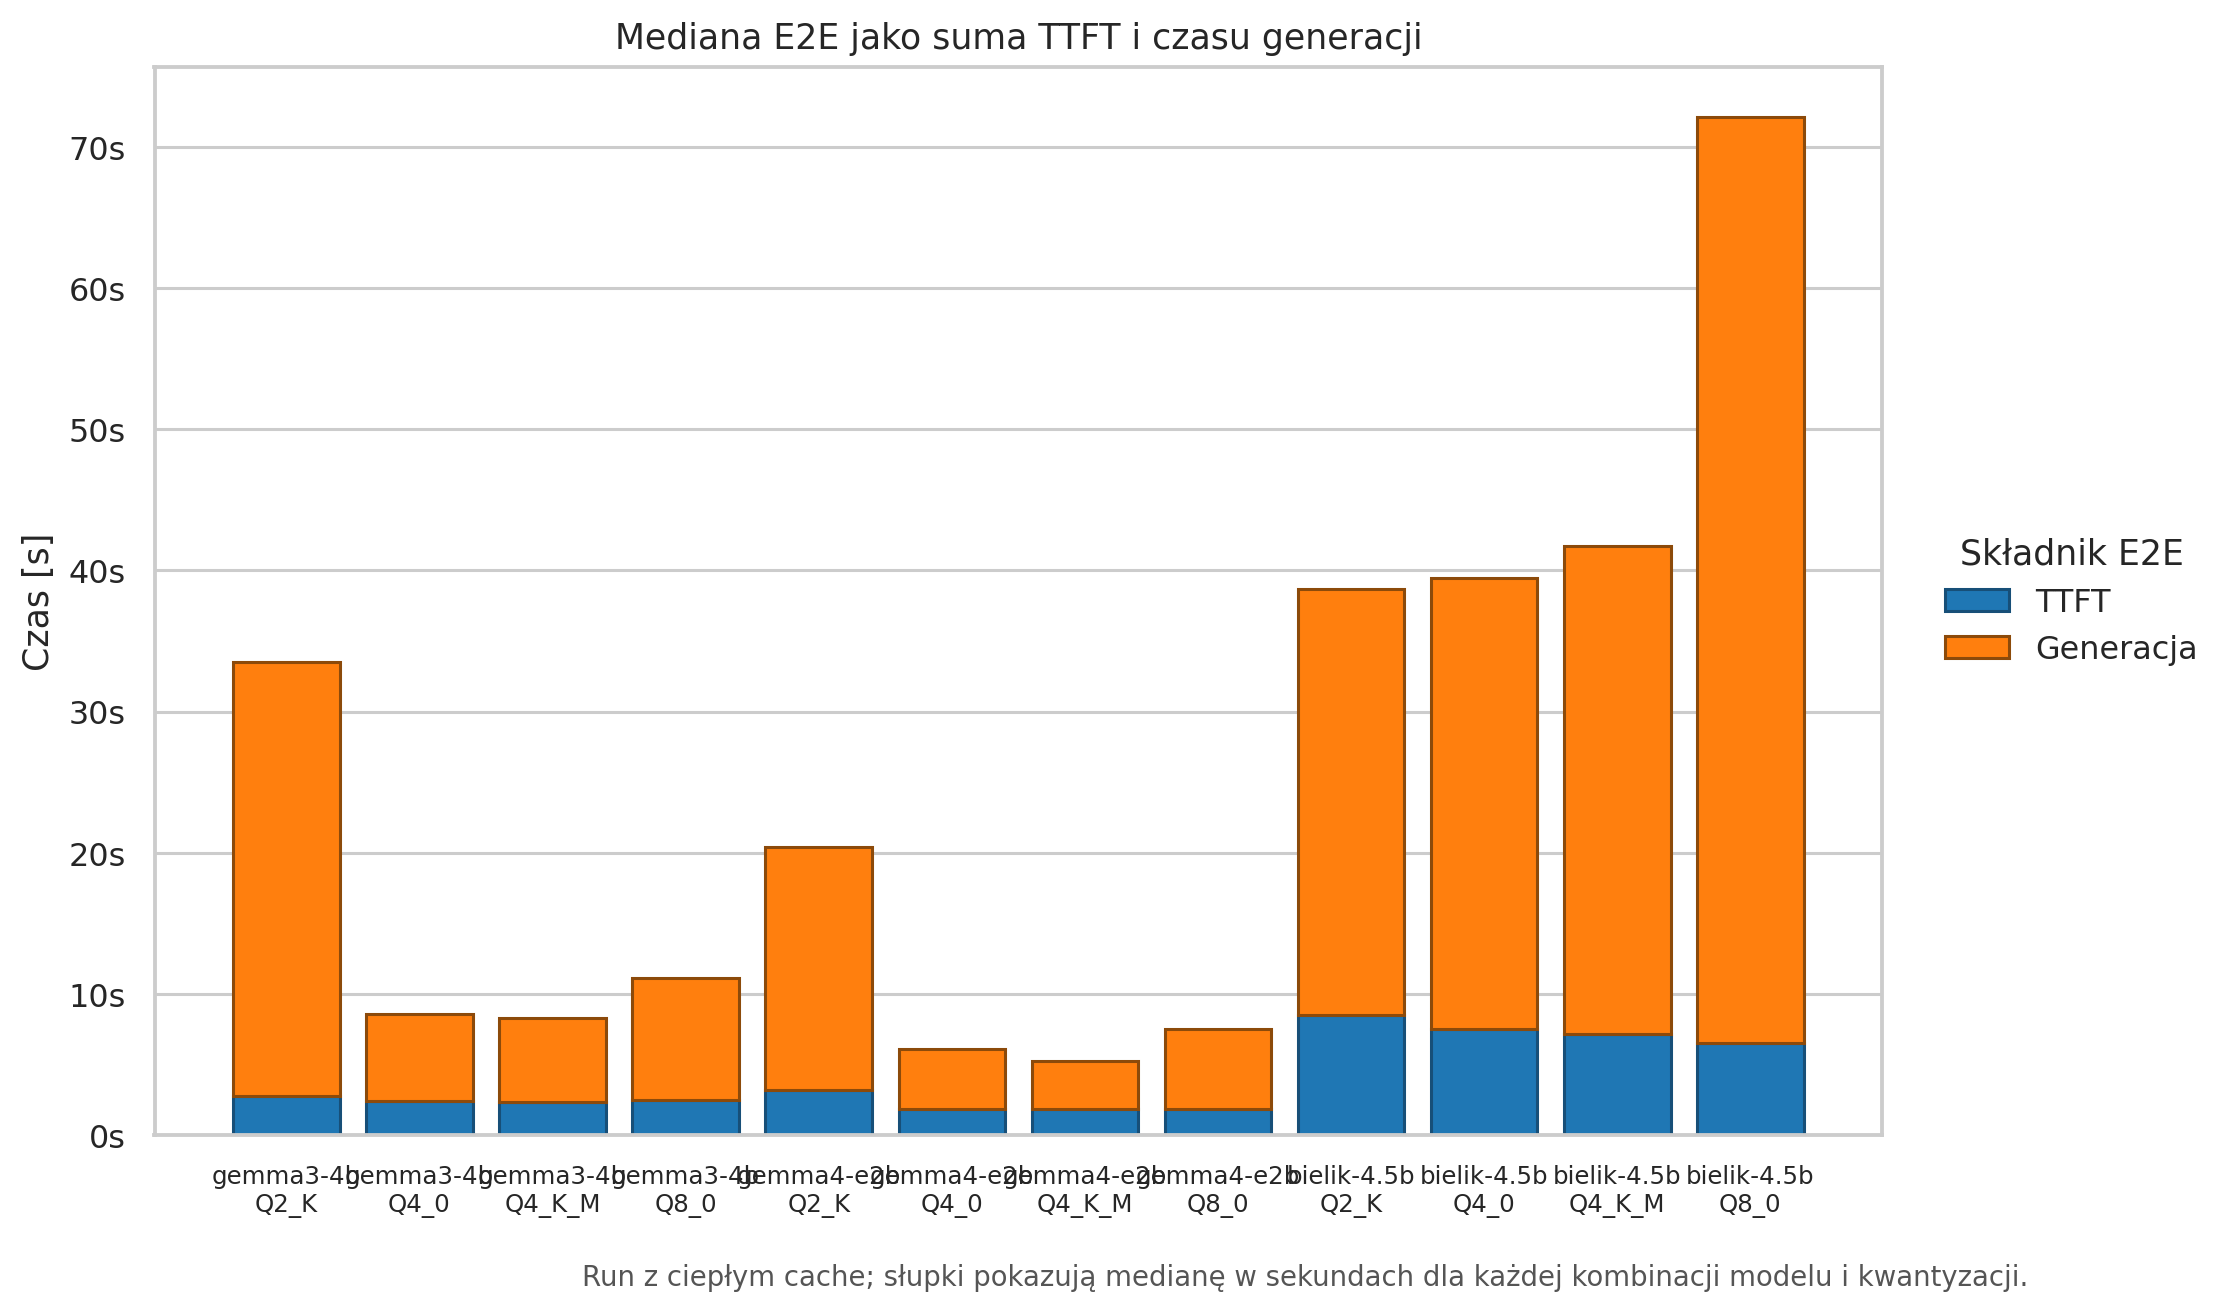
\includegraphics[width=0.95\textwidth]{03_dekompozycja_e2e.png}
  \caption{Dekompozycja E2E na TTFT i~\emph{generation\_ms} (warm cache).
           Wysokości słupków to mediany modelu log-normalnego $e^{\hat\mu}$
           ($n\approx 100$). Kwantyzacja wpływa głównie na czas generacji.}
  \label{fig:dekompozycja_e2e}
\end{figure}

\begin{figure}[H]
  \centering
  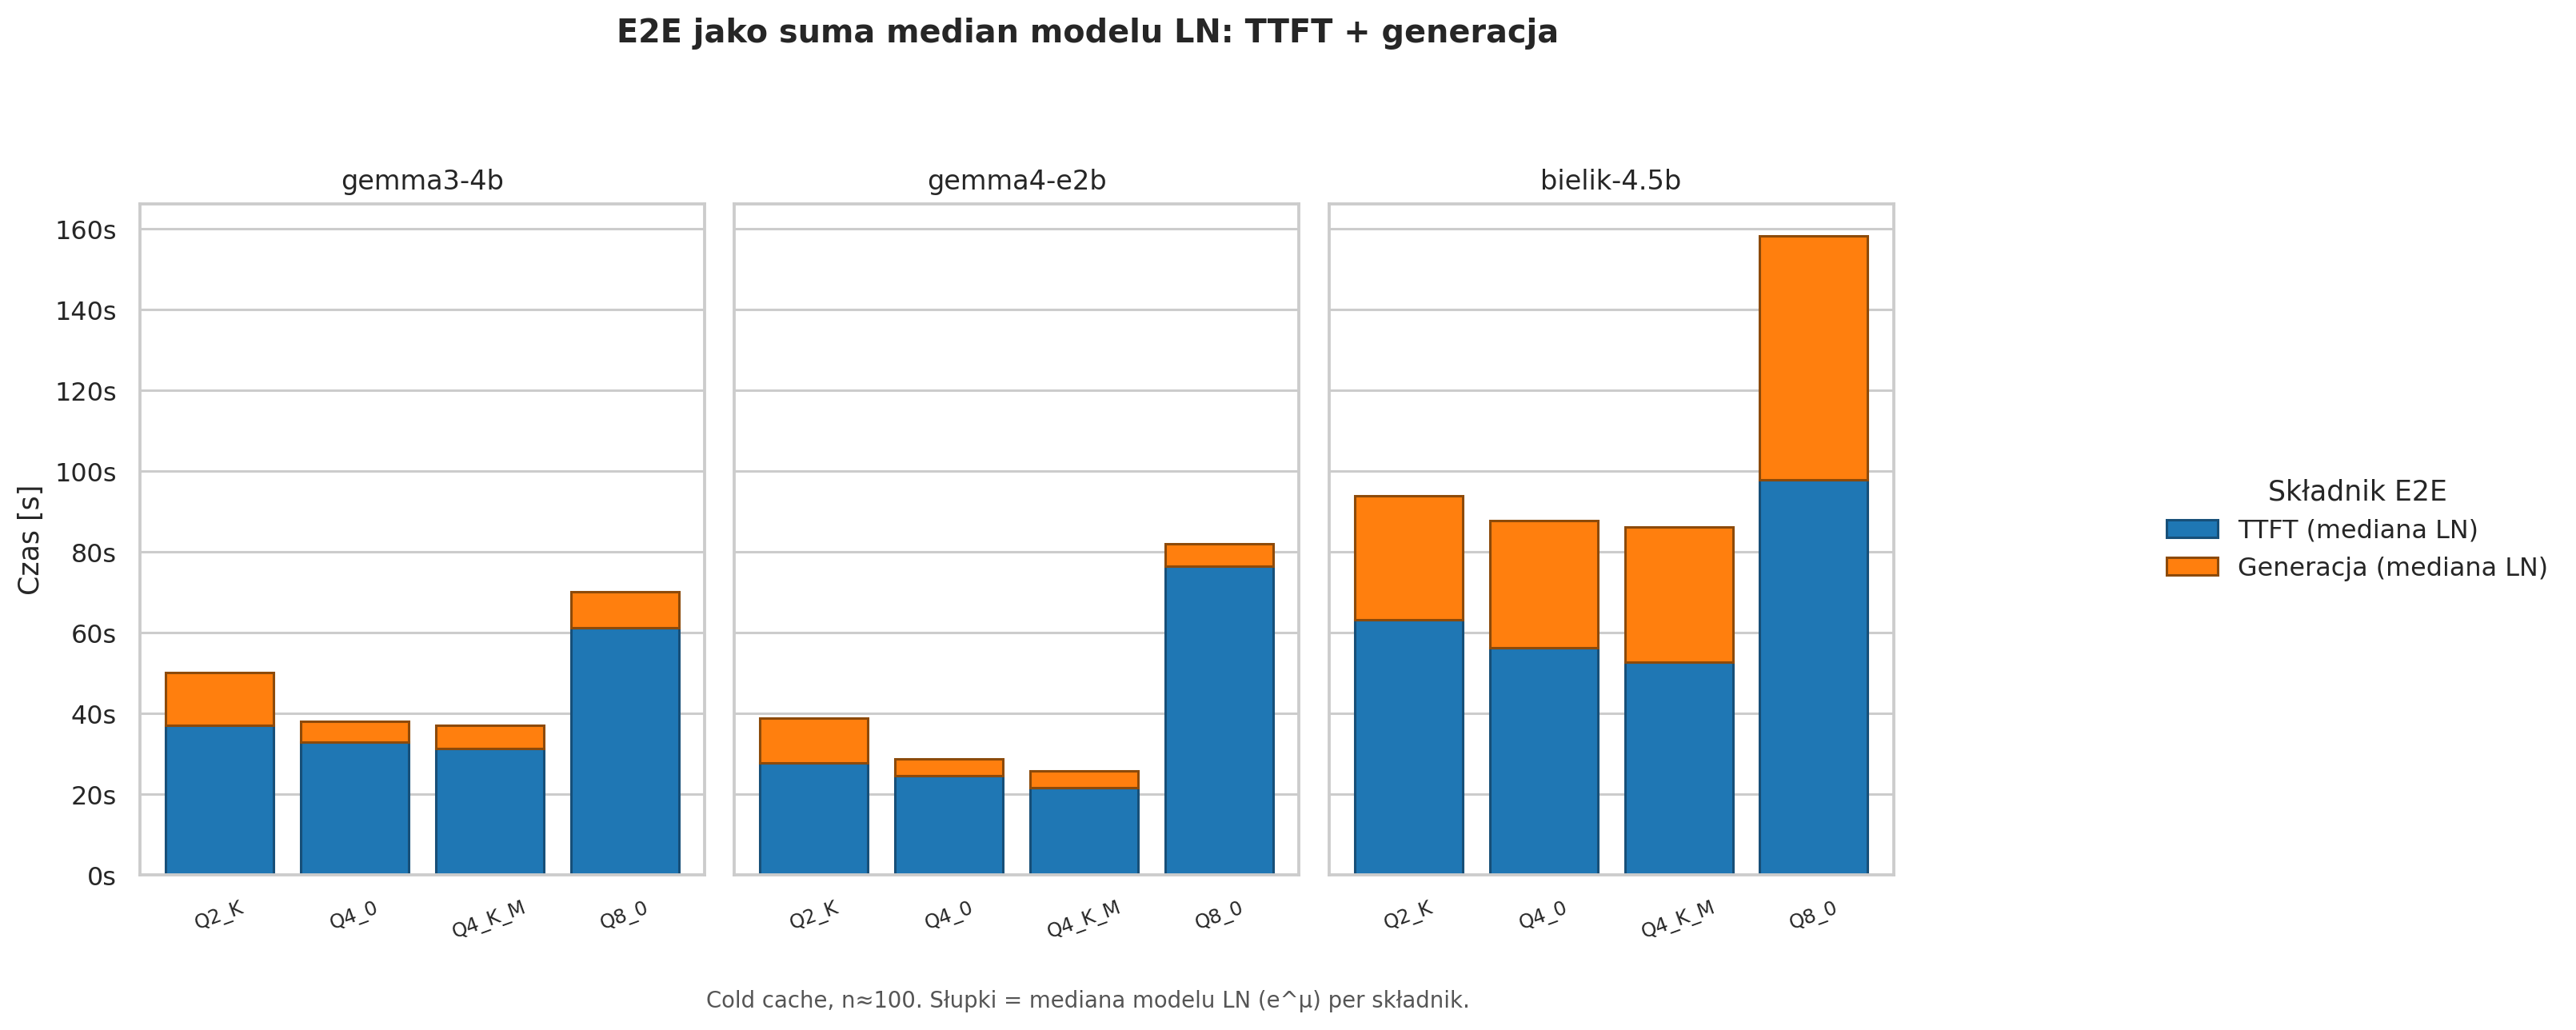
\includegraphics[width=0.95\textwidth]{cold_03_dekompozycja_e2e.png}
  \caption{Dekompozycja E2E na TTFT i~\emph{generation\_ms} (cold cache).
           Mediany modelu LN $e^{\hat\mu}$, $n\approx 100$. Prefill dominuje
           budżet czasu.}
  \label{fig:cold_dekompozycja_e2e}
\end{figure}

\subsubsection{Model log-normalny dla czasów generacji}

Czasy generacji są dodatnie i~prawostronnie skośne (różna długość odpowiedzi).
Przyjęto więc wspólny model roboczy log-normalny: lokalizacja
$e^{\hat\mu}$ (mediana modelu LN), przedział $e^{\hat\mu\pm\hat\sigma}$.
Rysunek~\ref{fig:warm_ln_fit} pokazuje histogramy \emph{generation} oraz
dopasowaną gęstość LN dla warm cache (analogicznie cold ---
rysunek~\ref{fig:cold_ln_fit}).

\begin{figure}[H]
  \centering
  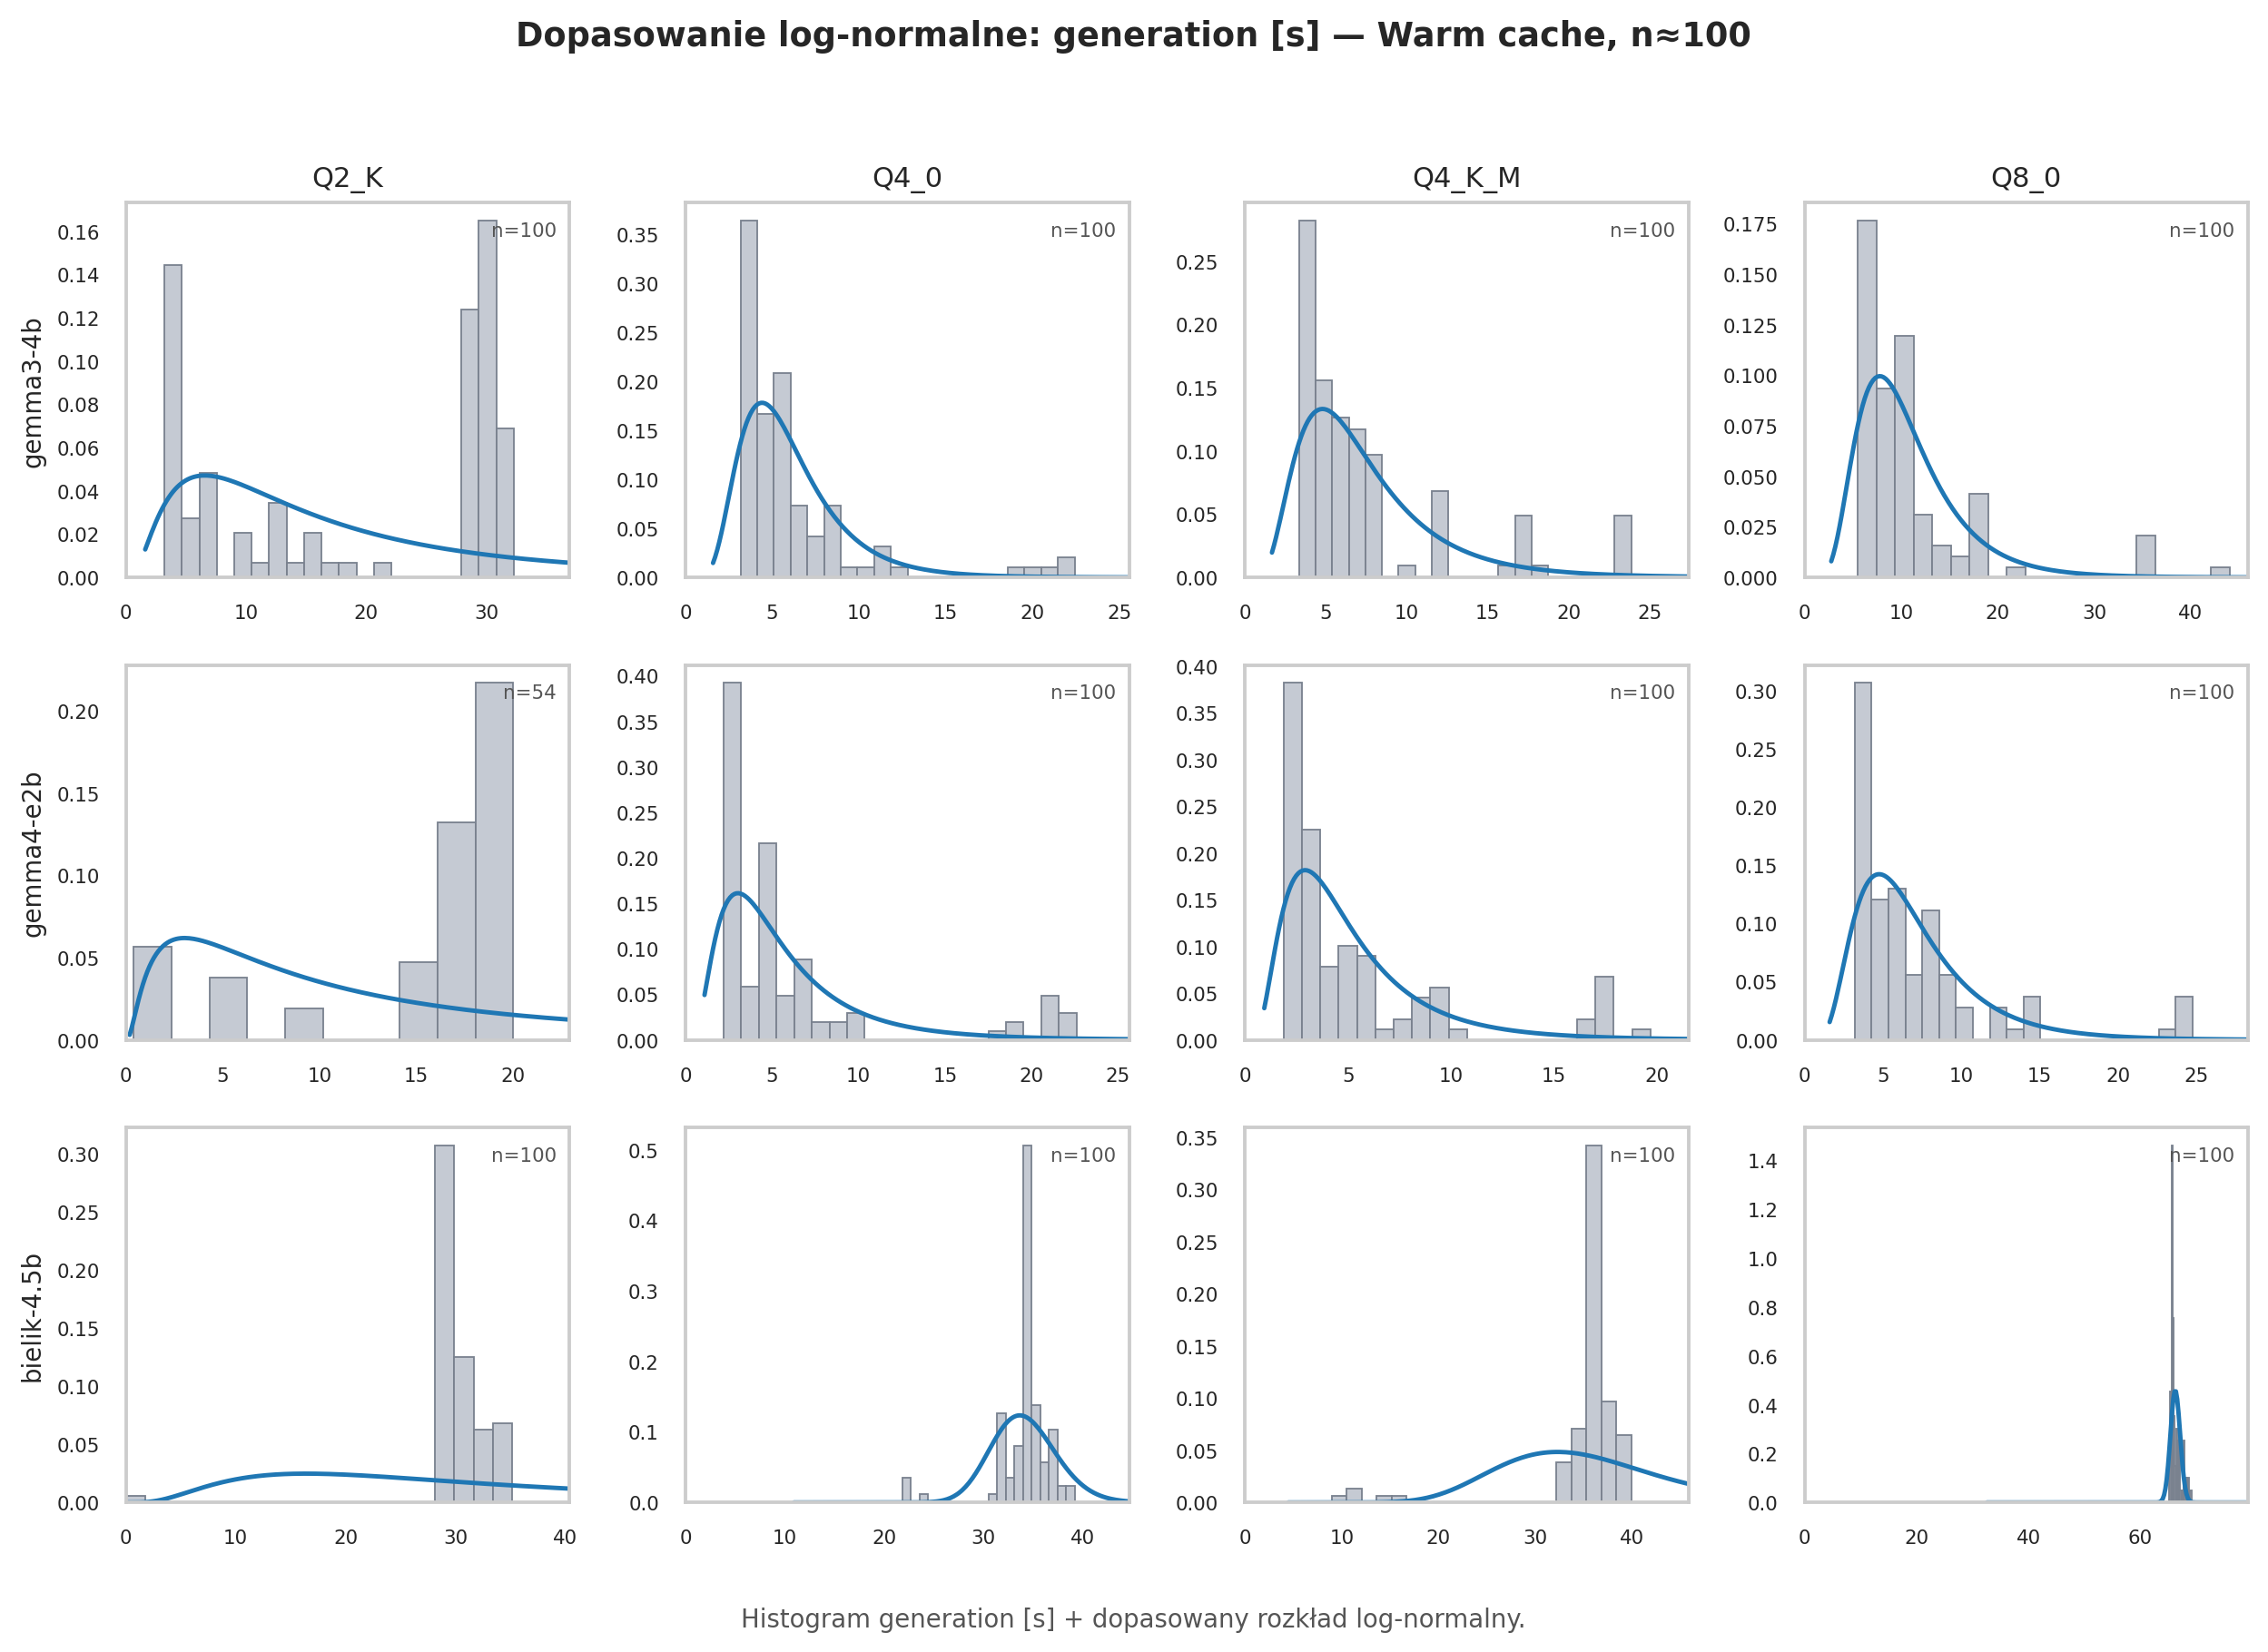
\includegraphics[width=0.95\textwidth]{warm_generation_ln_fit_matrix.png}
  \caption{Dopasowanie rozkładu log-normalnego do \emph{generation\_ms}
           (warm cache, $n\approx 100$). Histogram oraz gęstość LN per model
           i~wariant kwantyzacji.}
  \label{fig:warm_ln_fit}
\end{figure}

\begin{figure}[H]
  \centering
  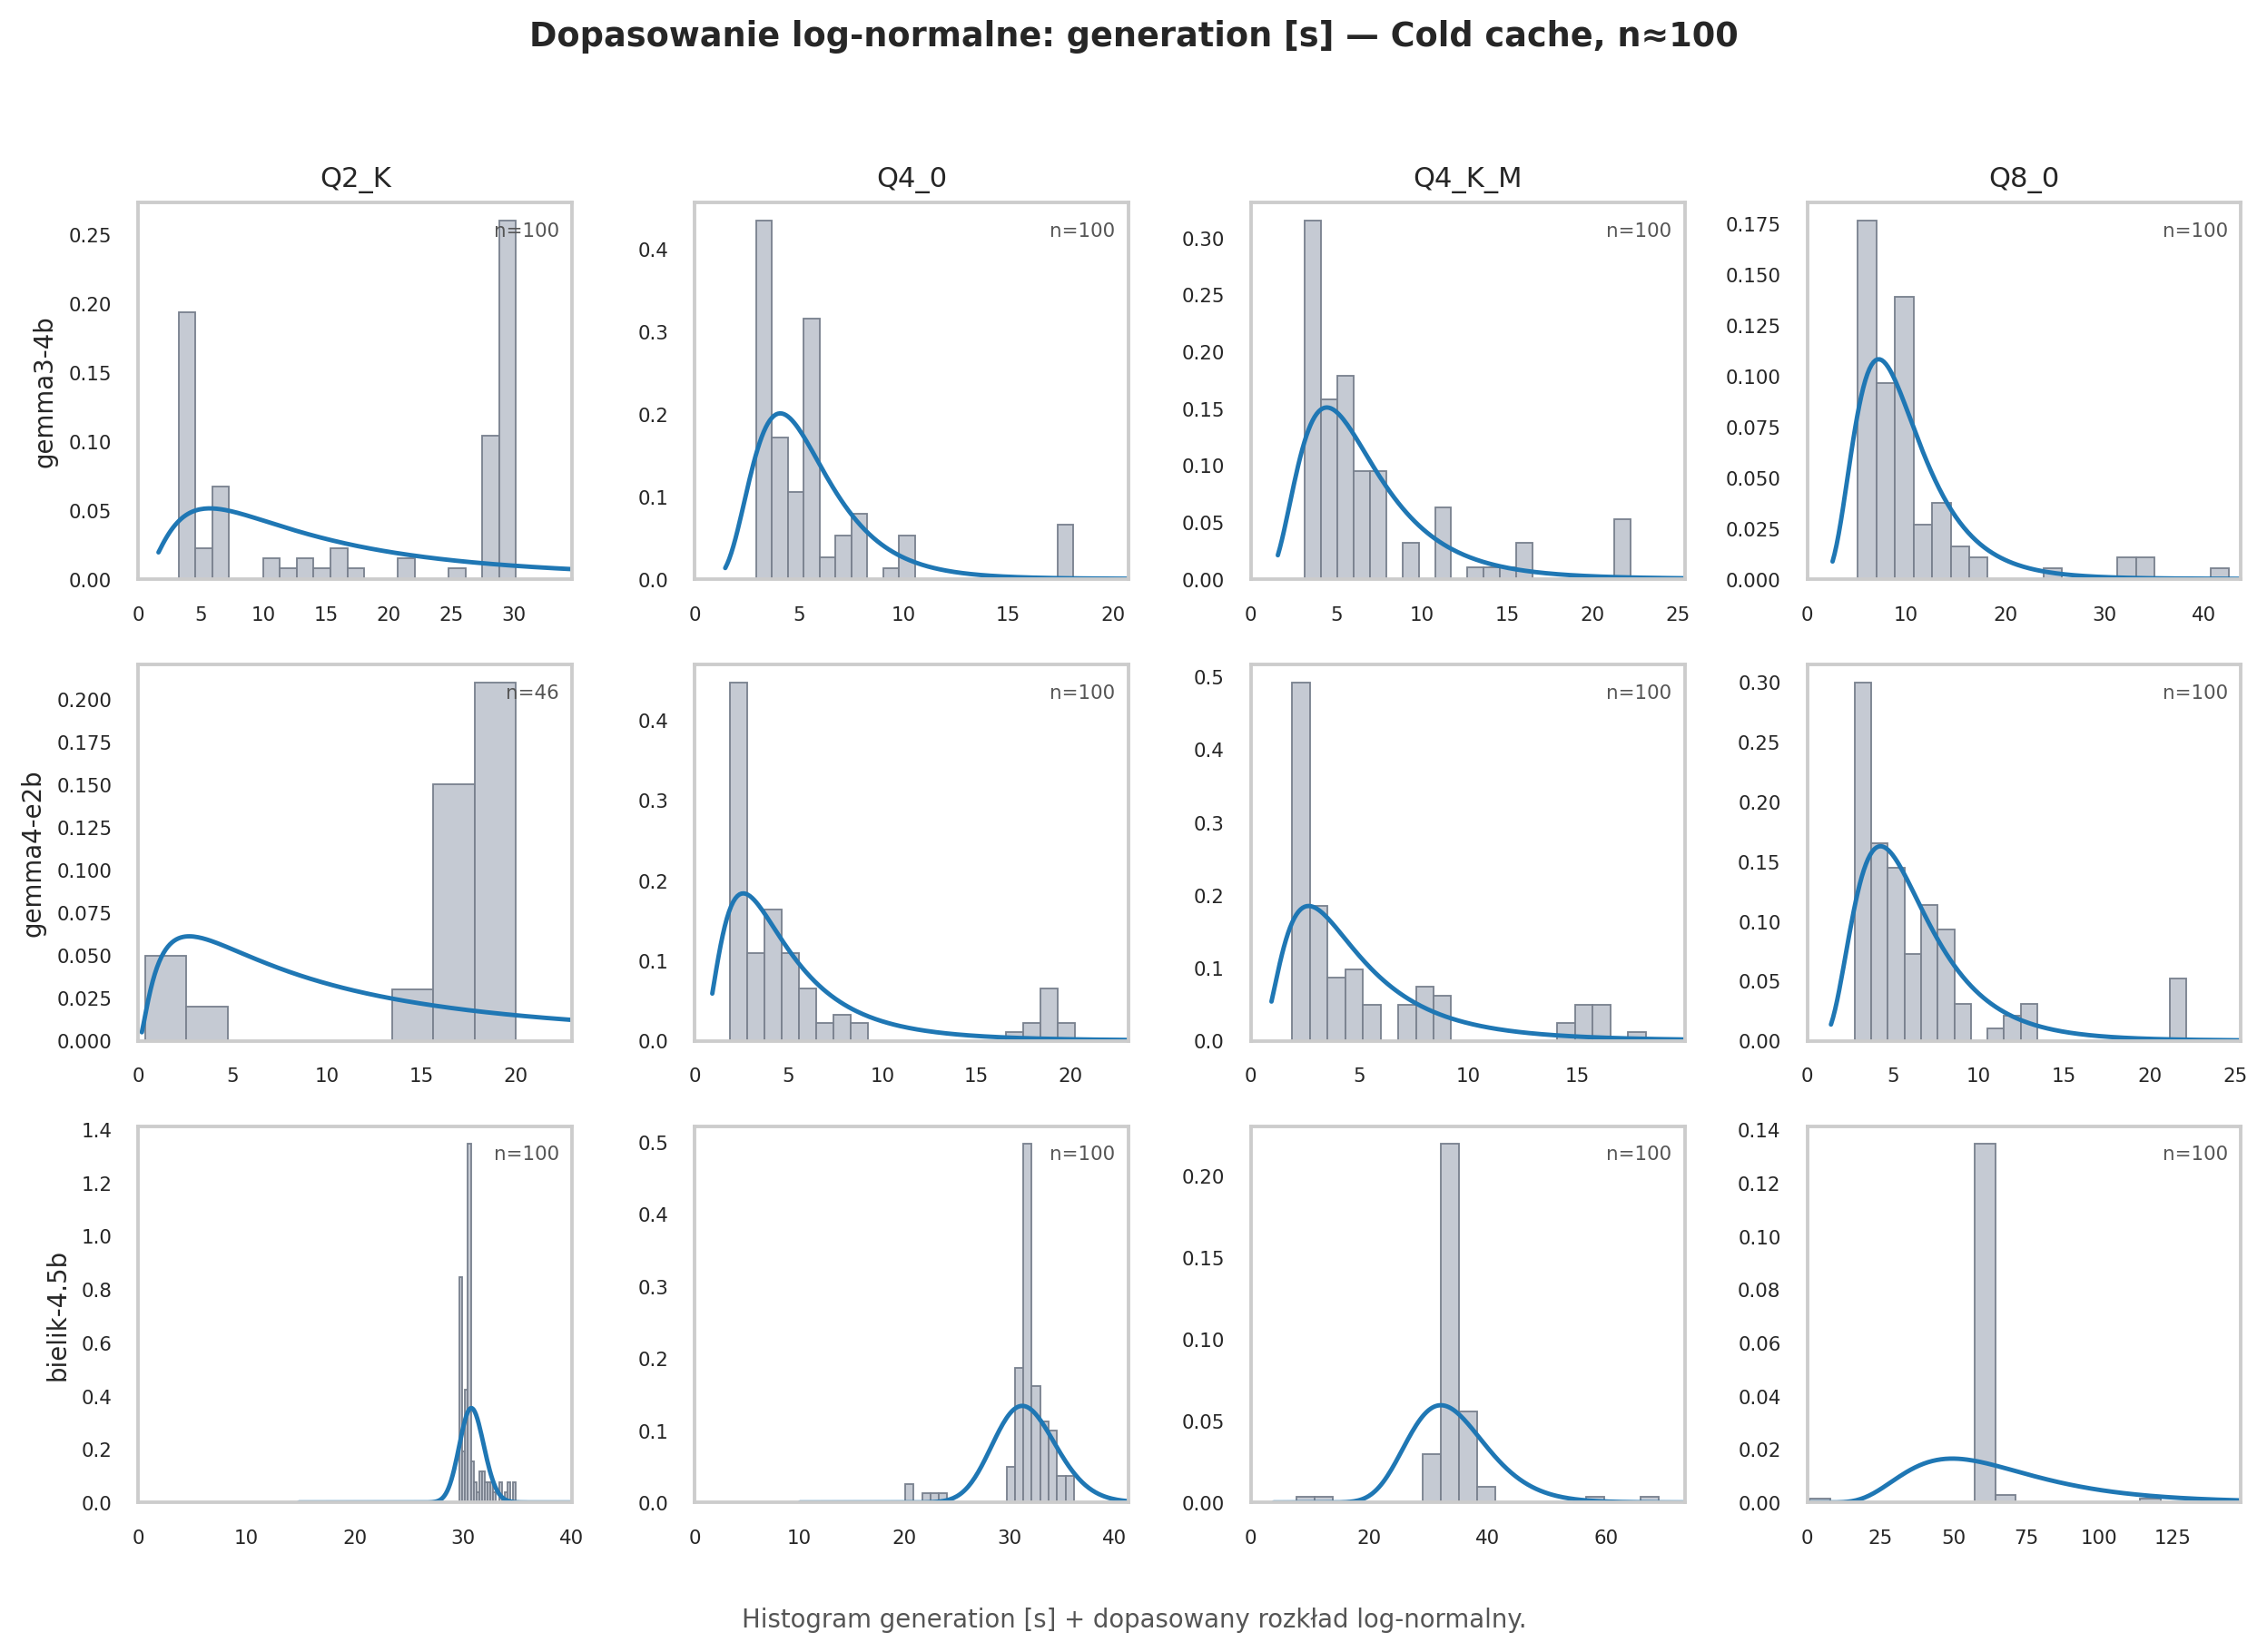
\includegraphics[width=0.95\textwidth]{cold_generation_ln_fit_matrix.png}
  \caption{Dopasowanie rozkładu log-normalnego do \emph{generation\_ms}
           (cold cache, $n\approx 100$).}
  \label{fig:cold_ln_fit}
\end{figure}

\subsubsection{Wyniki warm-cache}

Tabela~\ref{tab:kwantyzacja_wyniki} zestawia mediany modelu LN dla TTFT,
generacji i~E2E oraz przyspieszenie generacji względem Q8\_0
($\mathrm{speedup}= e^{\hat\mu_{\mathrm{Q8}}}/e^{\hat\mu_{\mathrm{wariant}}}$).

\begin{table}[H]
  \centering
  \caption{Wyniki kwantyzacji warm-cache: mediany modelu LN ($e^{\hat\mu}$)
           oraz przyspieszenie generacji względem Q8\_0 ($n\approx 100$).}
  \label{tab:kwantyzacja_wyniki}
  \small
  \begin{tabular}{llccccc}
    \hline
    Model & Wariant & GGUF & TTFT & Gen & E2E & Speedup \\
    \hline
    \texttt{gemma3-4b}  & Q2\_K   & 1{,}61G & 2{,}74s & 14{,}18s & 17{,}74s & 0{,}68$\times$ \\
    \texttt{gemma3-4b}  & Q4\_0   & 2{,}20G & 2{,}52s & 5{,}44s  & 8{,}06s  & 1{,}77$\times$ \\
    \texttt{gemma3-4b}  & Q4\_K\_M& 2{,}32G & 2{,}44s & 6{,}42s  & 9{,}02s  & 1{,}50$\times$ \\
    \texttt{gemma3-4b}  & Q8\_0   & 3{,}85G & 2{,}51s & 9{,}66s  & 12{,}30s & 1{,}00$\times$ \\
    \texttt{gemma4-e2b} & Q2\_K   & 2{,}78G & 3{,}08s & 10{,}79s & 16{,}44s & 0{,}57$\times$ \\
    \texttt{gemma4-e2b} & Q4\_0   & 3{,}13G & 1{,}93s & 4{,}67s  & 6{,}80s  & 1{,}33$\times$ \\
    \texttt{gemma4-e2b} & Q4\_K\_M& 3{,}19G & 1{,}83s & 4{,}29s  & 6{,}30s  & 1{,}45$\times$ \\
    \texttt{gemma4-e2b} & Q8\_0   & 4{,}63G & 1{,}88s & 6{,}20s  & 8{,}22s  & 1{,}00$\times$ \\
    \texttt{bielik-4.5b}& Q2\_K   & 1{,}65G & 8{,}58s & 28{,}51s & 39{,}19s & 2{,}32$\times$ \\
    \texttt{bielik-4.5b}& Q4\_0   & 2{,}52G & 7{,}59s & 34{,}00s & 41{,}64s & 1{,}95$\times$ \\
    \texttt{bielik-4.5b}& Q4\_K\_M& 2{,}68G & 7{,}06s & 34{,}36s & 41{,}67s & 1{,}93$\times$ \\
    \texttt{bielik-4.5b}& Q8\_0   & 4{,}71G & 6{,}54s & 66{,}22s & 72{,}78s & 1{,}00$\times$ \\
    \hline
  \end{tabular}
\end{table}

\begin{figure}[H]
  \centering
  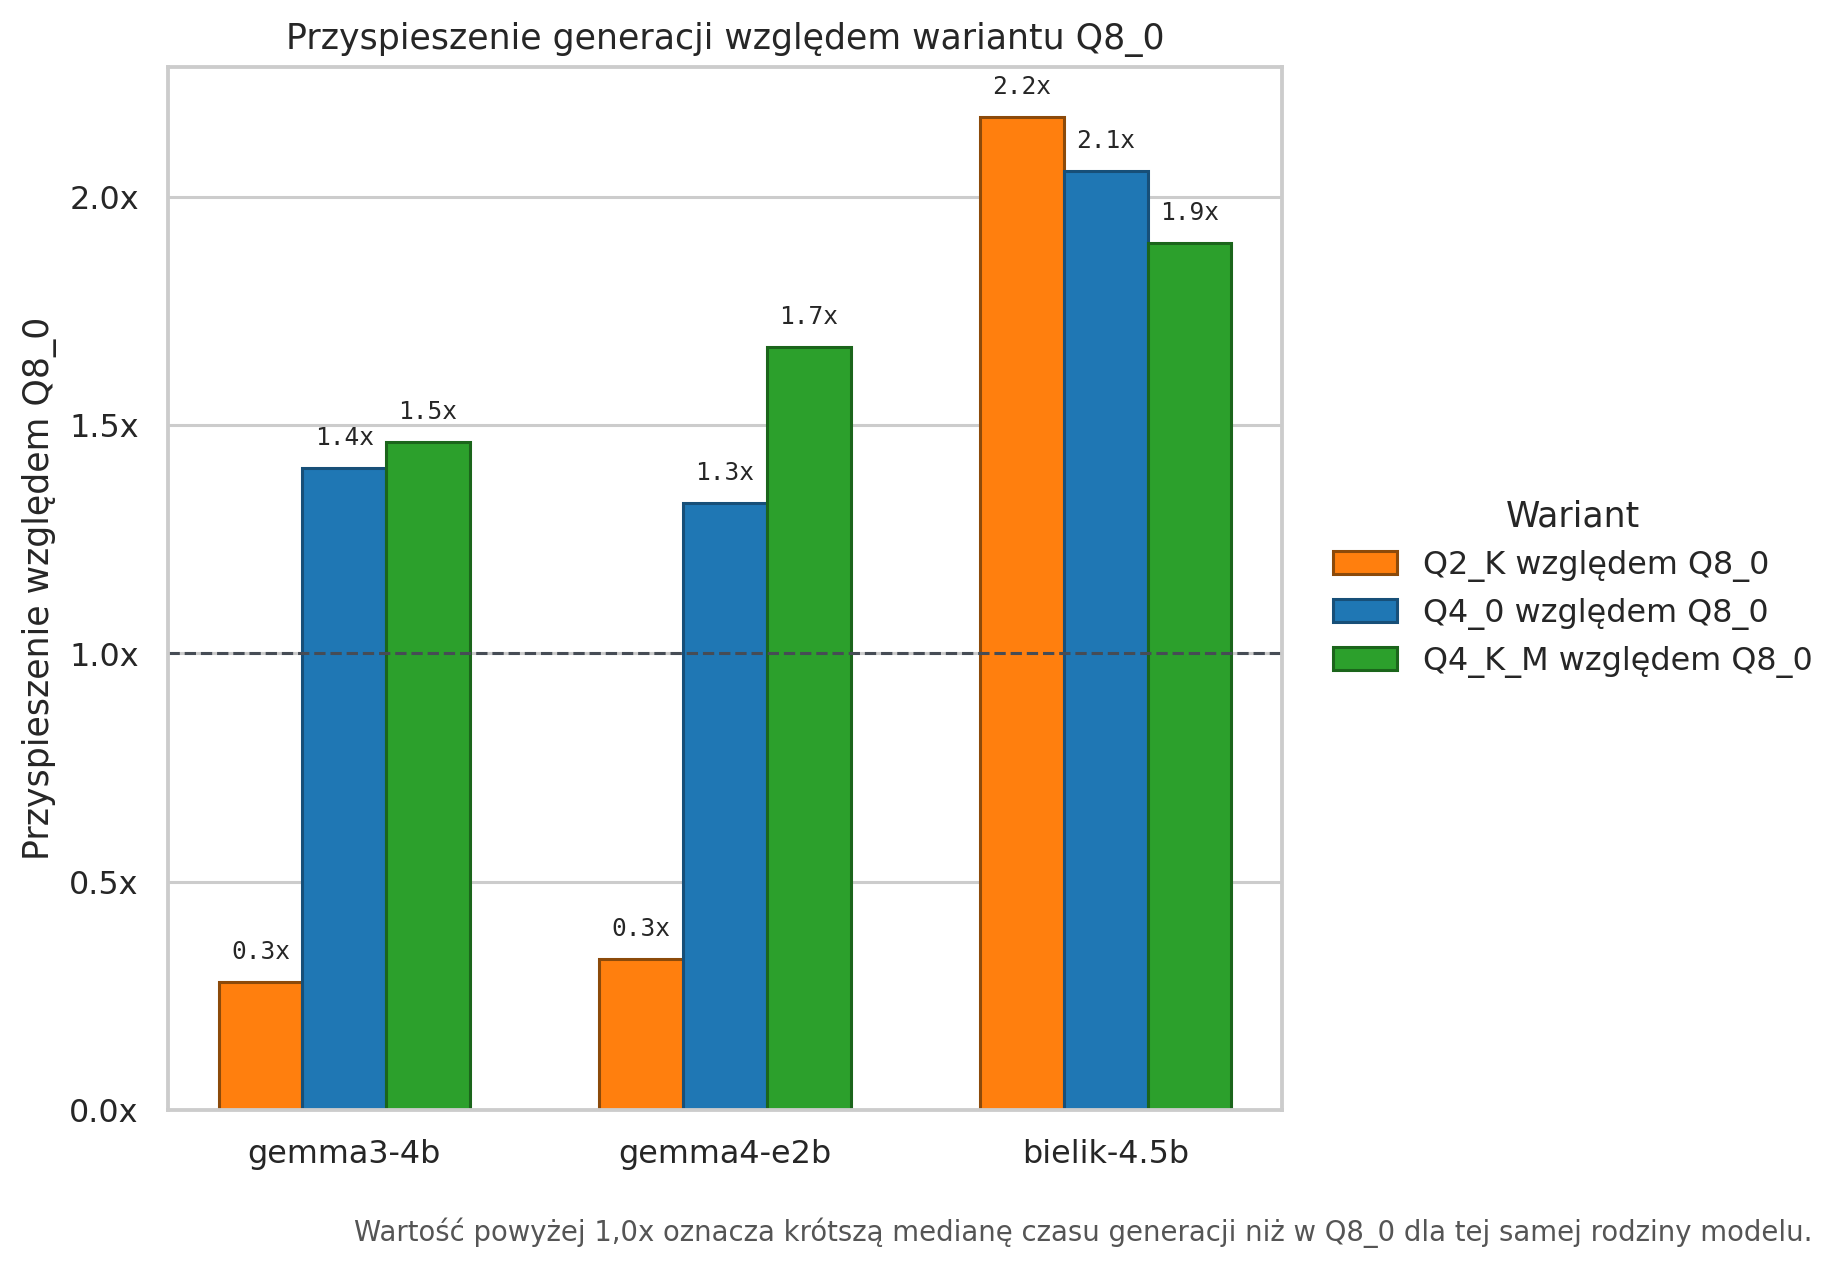
\includegraphics[width=0.85\textwidth]{04_przyspieszenie_wzgledem_q8.png}
  \caption{Przyspieszenie \emph{generation\_ms} względem Q8\_0 (warm cache).
           Speedup $= e^{\hat\mu_{\mathrm{Q8}}}/e^{\hat\mu_{\mathrm{wariant}}}$.}
  \label{fig:speedup_q8}
\end{figure}

\begin{figure}[H]
  \centering
  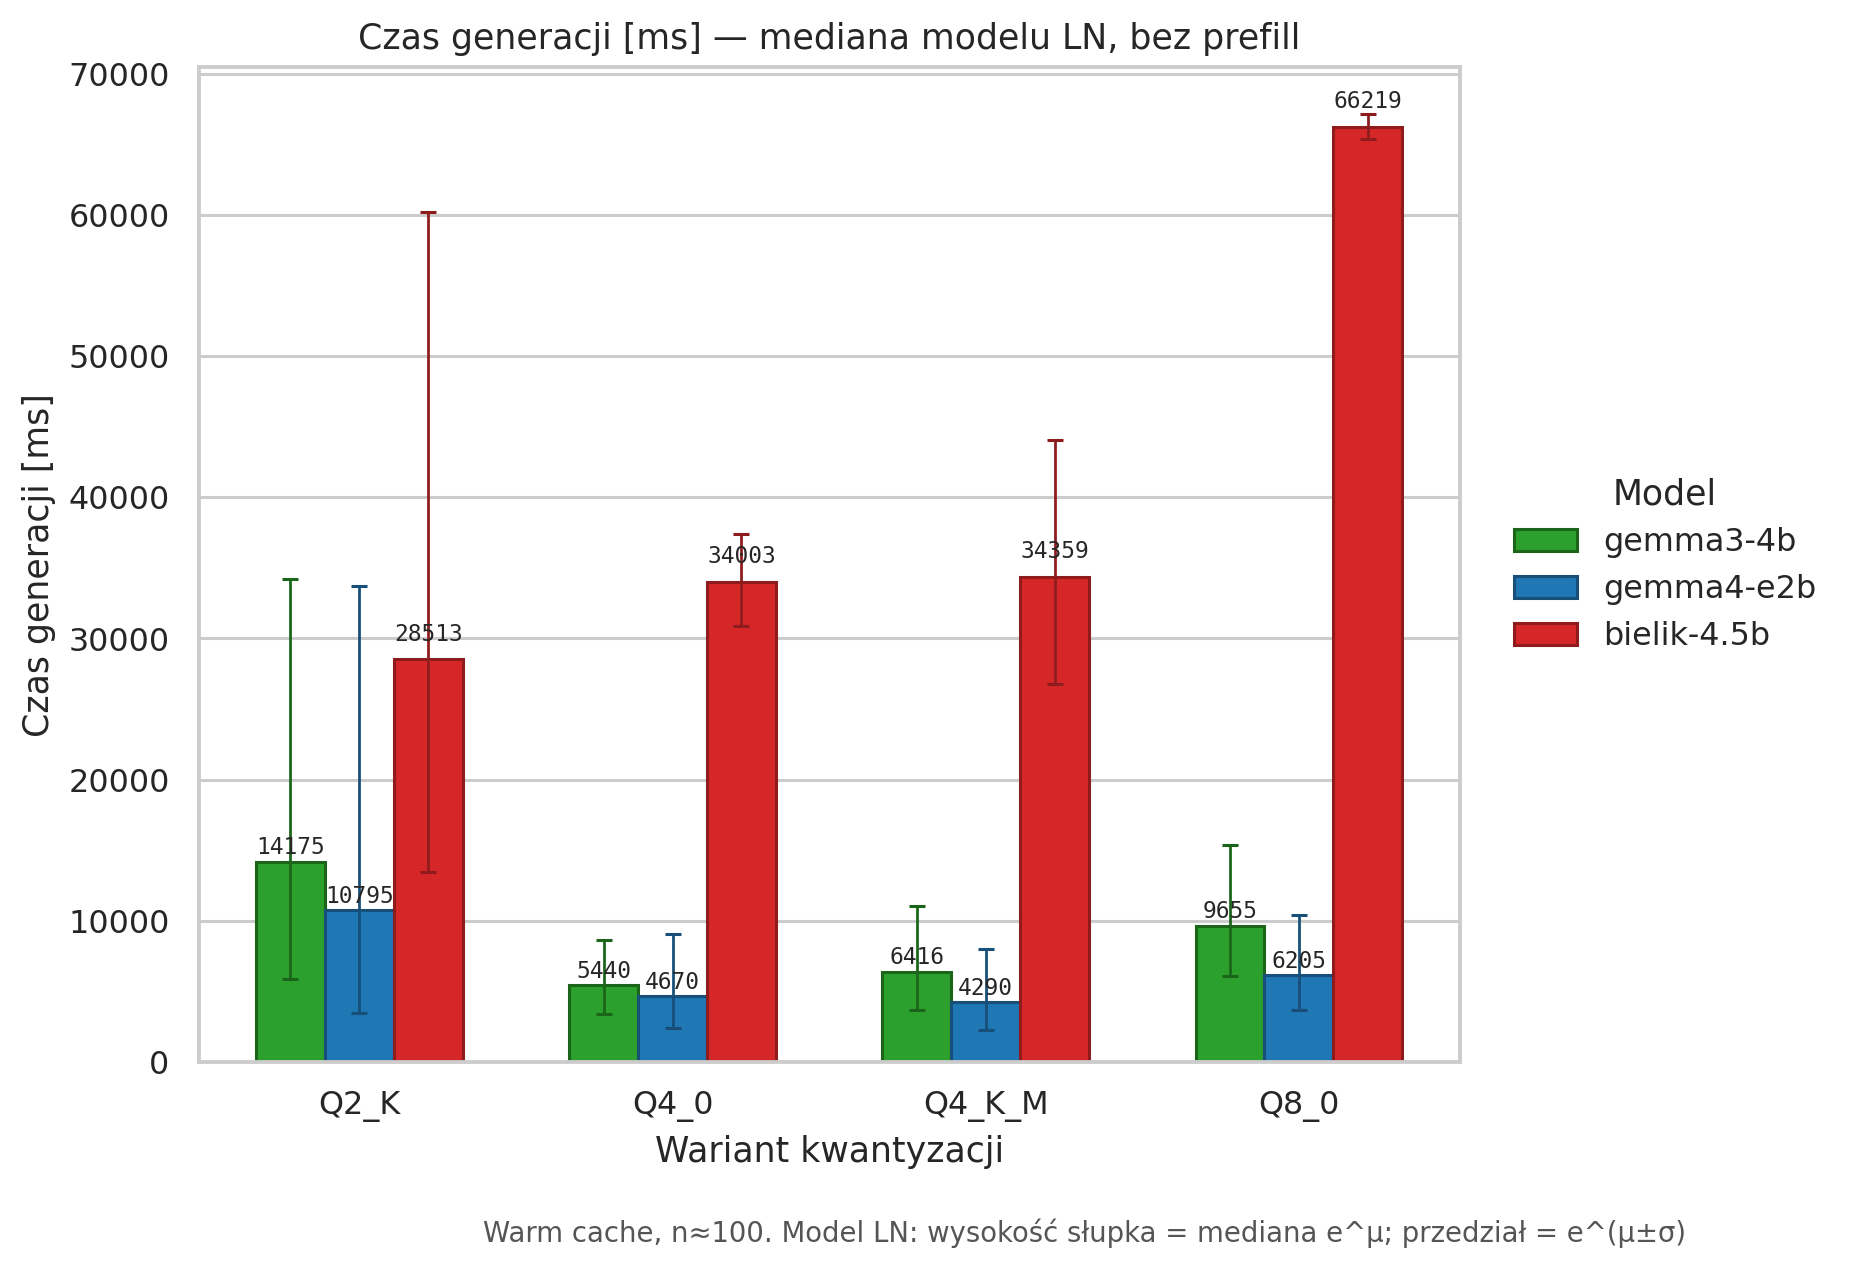
\includegraphics[width=0.85\textwidth]{07_generation_ms_wedlug_wariantu.png}
  \caption{Czas \emph{generation\_ms} według wariantu kwantyzacji
           (mediana modelu LN $e^{\hat\mu}$, przedział $e^{\hat\mu\pm\hat\sigma}$;
           warm cache, $n\approx 100$).}
  \label{fig:gen_ms_variant}
\end{figure}

\begin{figure}[H]
  \centering
  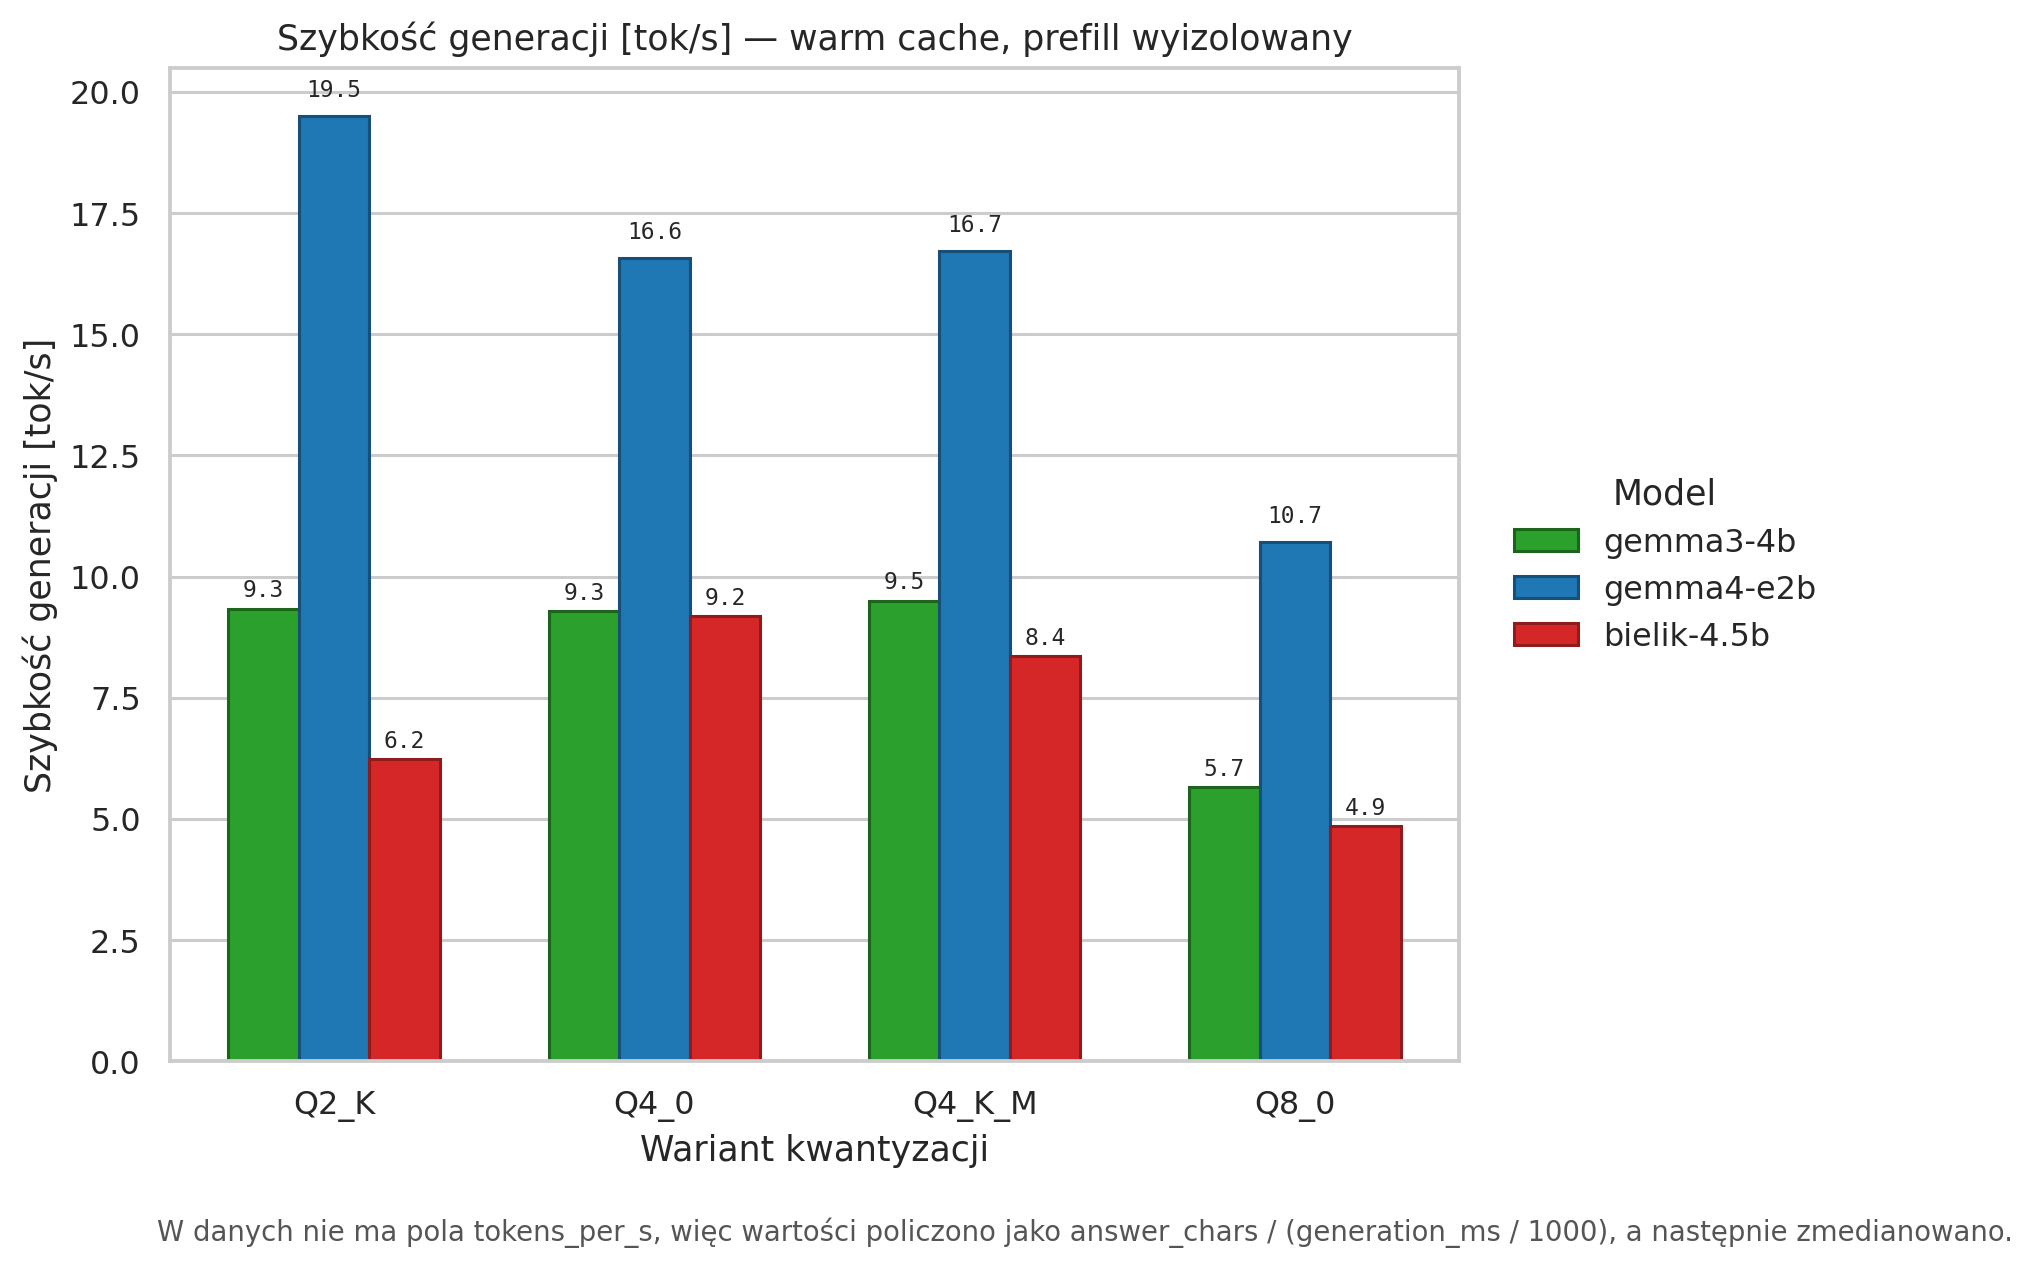
\includegraphics[width=0.85\textwidth]{08_szybkosc_generacji_tok_s_wedlug_wariantu.png}
  \caption{Szybkość generacji [znaki/s] (proxy tok/s) według wariantu
           kwantyzacji. Mediana modelu LN na per-rekord
           $\mathrm{answer\_chars}/(\mathrm{generation\_ms}/1000)$.}
  \label{fig:tok_s_variant}
\end{figure}

\subsubsection{Anomalie i wnioski}
\label{subsubsec:anomalie}

\textbf{Anomalia Q2\_K.} Wariant \texttt{gemma3-4b/Q2\_K} ma długi czas
generacji mimo małego pliku GGUF: przy niskiej precyzji wag model produkuje
rozwlekłe odpowiedzi (rysunek~\ref{fig:gen_vs_length}).

\begin{figure}[H]
  \centering
  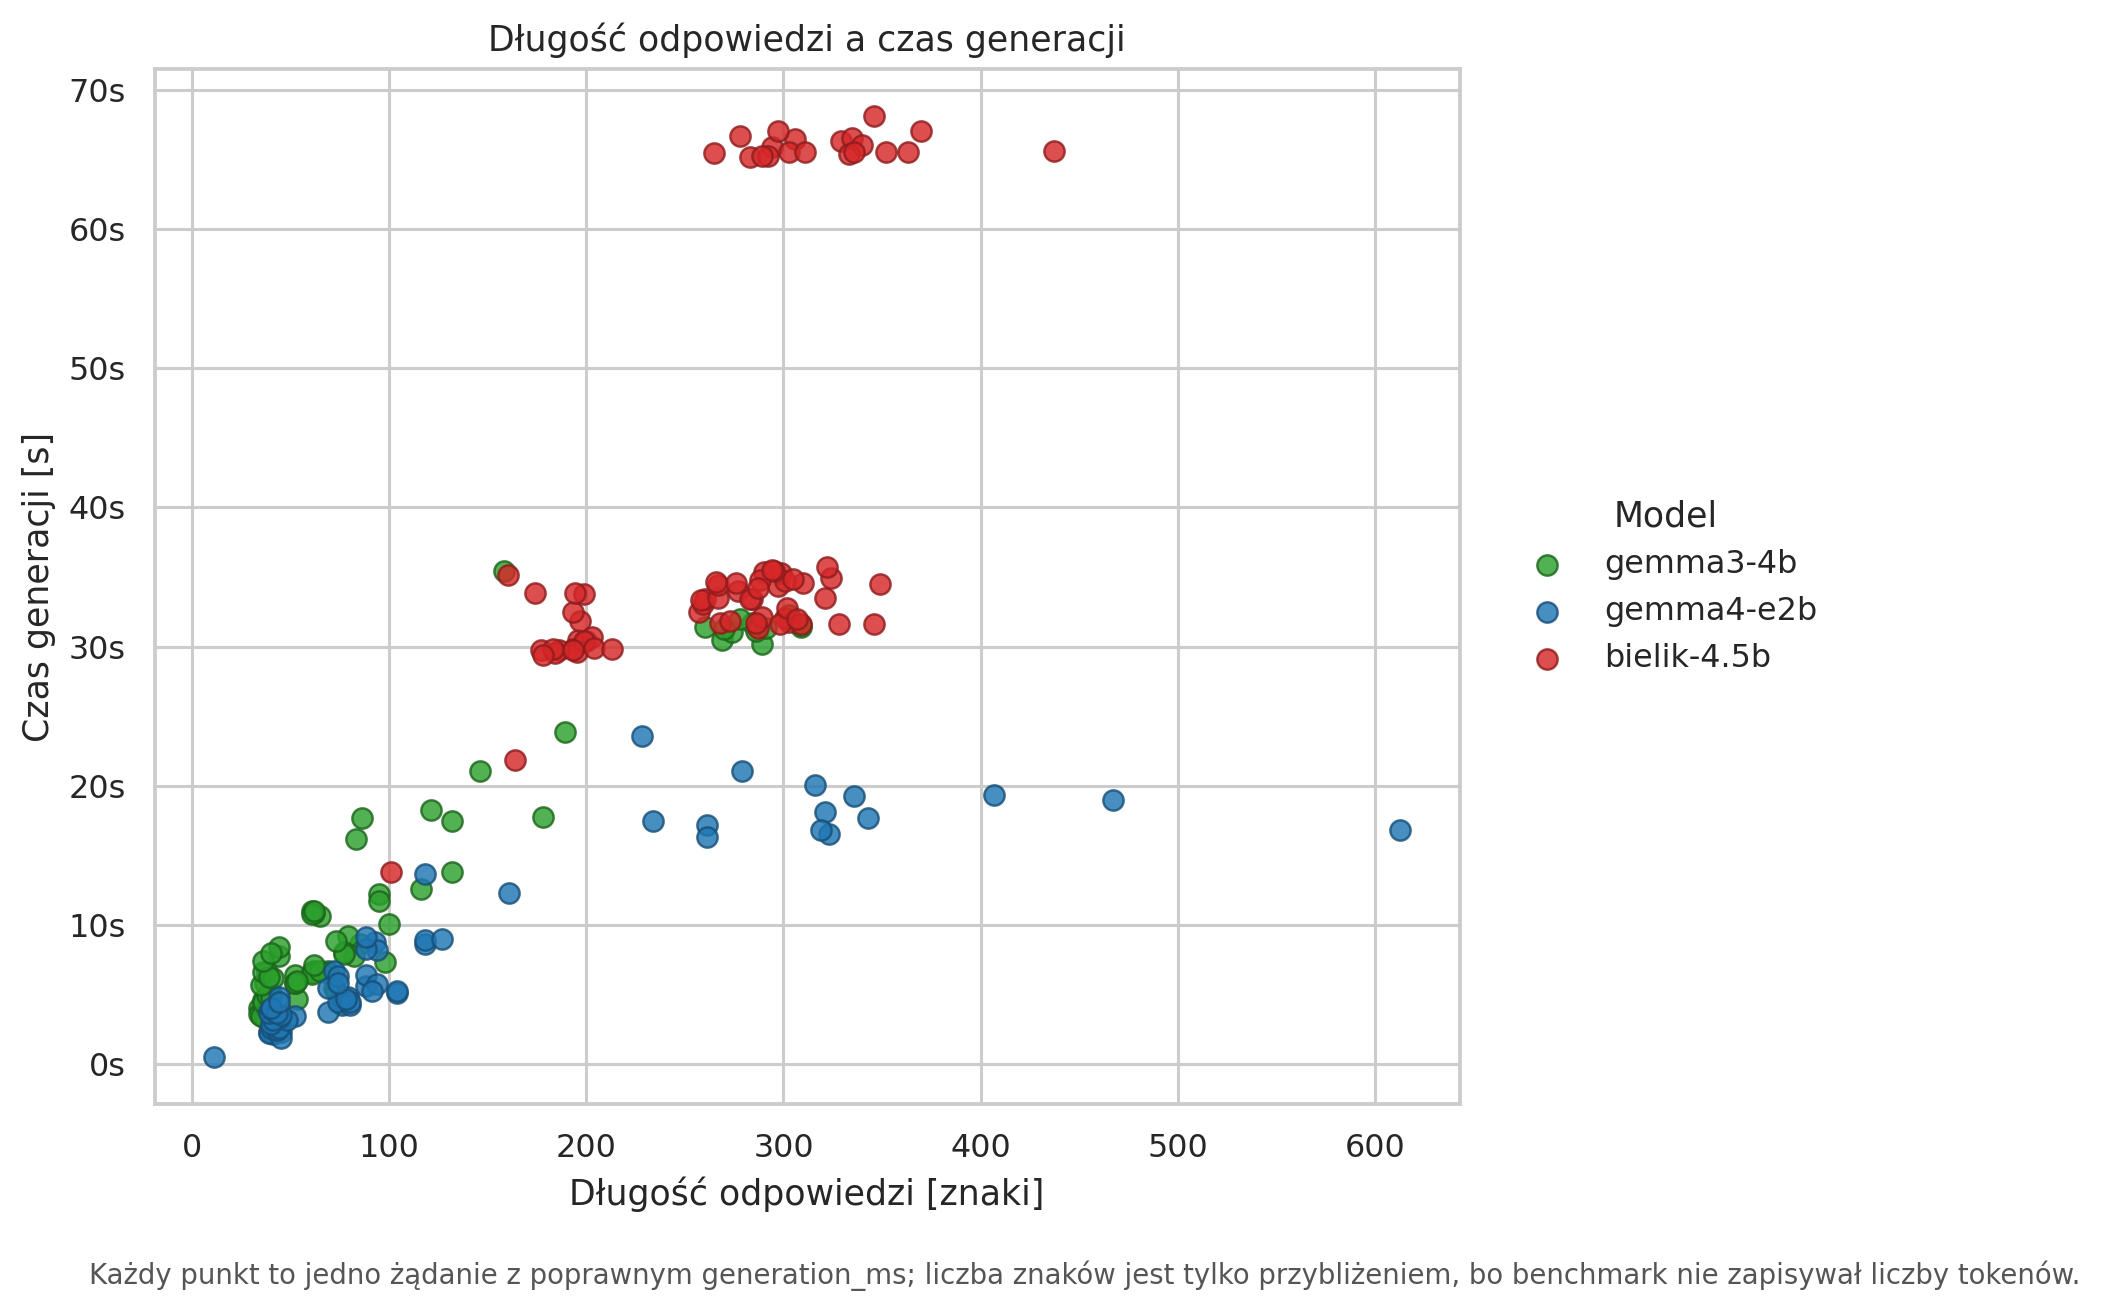
\includegraphics[width=0.85\textwidth]{05_generacja_a_dlugosc_odpowiedzi.png}
  \caption{Zależność czasu generacji od długości odpowiedzi
           (anomalia Q2\_K; warm cache).}
  \label{fig:gen_vs_length}
\end{figure}

\textbf{Anomalia \texttt{gemma4-e2b/Q2\_K}.} Model MoE jest wrażliwy na
kwantyzację 2-bitową (część pustych odpowiedzi / niższy hit rate cache).

\textbf{Odrzucenie Bielika.} Nawet przy Q4\_K\_M mediana LN generacji wynosi
ok.~34~s --- rzędu $5\times$ wolniej niż \texttt{gemma3-4b/Q4\_K\_M}. Model
nie jest wariantem produkcyjnym dla asystenta głosowego w~tym środowisku.

\textbf{Wniosek.} Q4\_K\_M to sensowny kompromis dla Gemm: dla
\texttt{gemma3-4b} ok.~$1{,}50\times$ przyspieszenie generacji względem Q8\_0
przy mniejszym pliku; dla \texttt{gemma4-e2b} ok.~$1{,}45\times$. Kwantyzacja
nie redukuje halucynacji --- to własność wag, nie precyzji reprezentacji.
Dalsza dźwignia opóźnienia to redukcja TTFT przez układanie promptu pod
\emph{prefix caching} (sekcja~\ref{subsec:prefix_caching}).


% ============================================================
\subsection{Prompt engineering i prefix caching}
\label{subsec:prefix_caching}
% ============================================================

\subsubsection{Problem: TTFT przy długim prompcie}

W~systemie Wilga \emph{system\_prompt} zawiera statyczny nagłówek (reguły,
instrukcje), blok sensoryczny oraz kontekst nauczyciela. Przy każdym zapytaniu
z~nowym kontekstem sensorycznym urządzenie musi wykonać prefill od zera.
W~protokole cold cache TTFT stanowi większość E2E; w~warm cache --- przy
stałym prefiksie --- TTFT spada o~rząd wielkości.

\subsubsection{Mechanizm prefix cachingu}

Podczas prefill model oblicza klucze~(K) i~wartości~(V). KV-cache może zostać
zachowane, jeśli tokeny od początku promptu są identyczne. Implikacja dla
architektury Teacher-Student (rozdział~3): statyczny blok musi być prefiksem,
a~zmienny (sensory, insight, pytanie) --- sufiksem.

\subsubsection{Empirycznie: cold vs warm TTFT}

Dla \texttt{gemma3-4b/Q4\_K\_M} mediana modelu LN TTFT wynosi ok.~31{,}3~s
w~cold cache oraz ok.~2{,}44~s w~warm cache
(rysunki~\ref{fig:cold_ttft},~\ref{fig:ttft_warm}). Redukcja
$(31{,}3 - 2{,}44)/31{,}3 \approx 92\%$. Porównanie dotyczy protokołów
cold vs warm przy tej samej siatce model$\times$wariant ($n\approx 100$).

\begin{figure}[H]
  \centering
  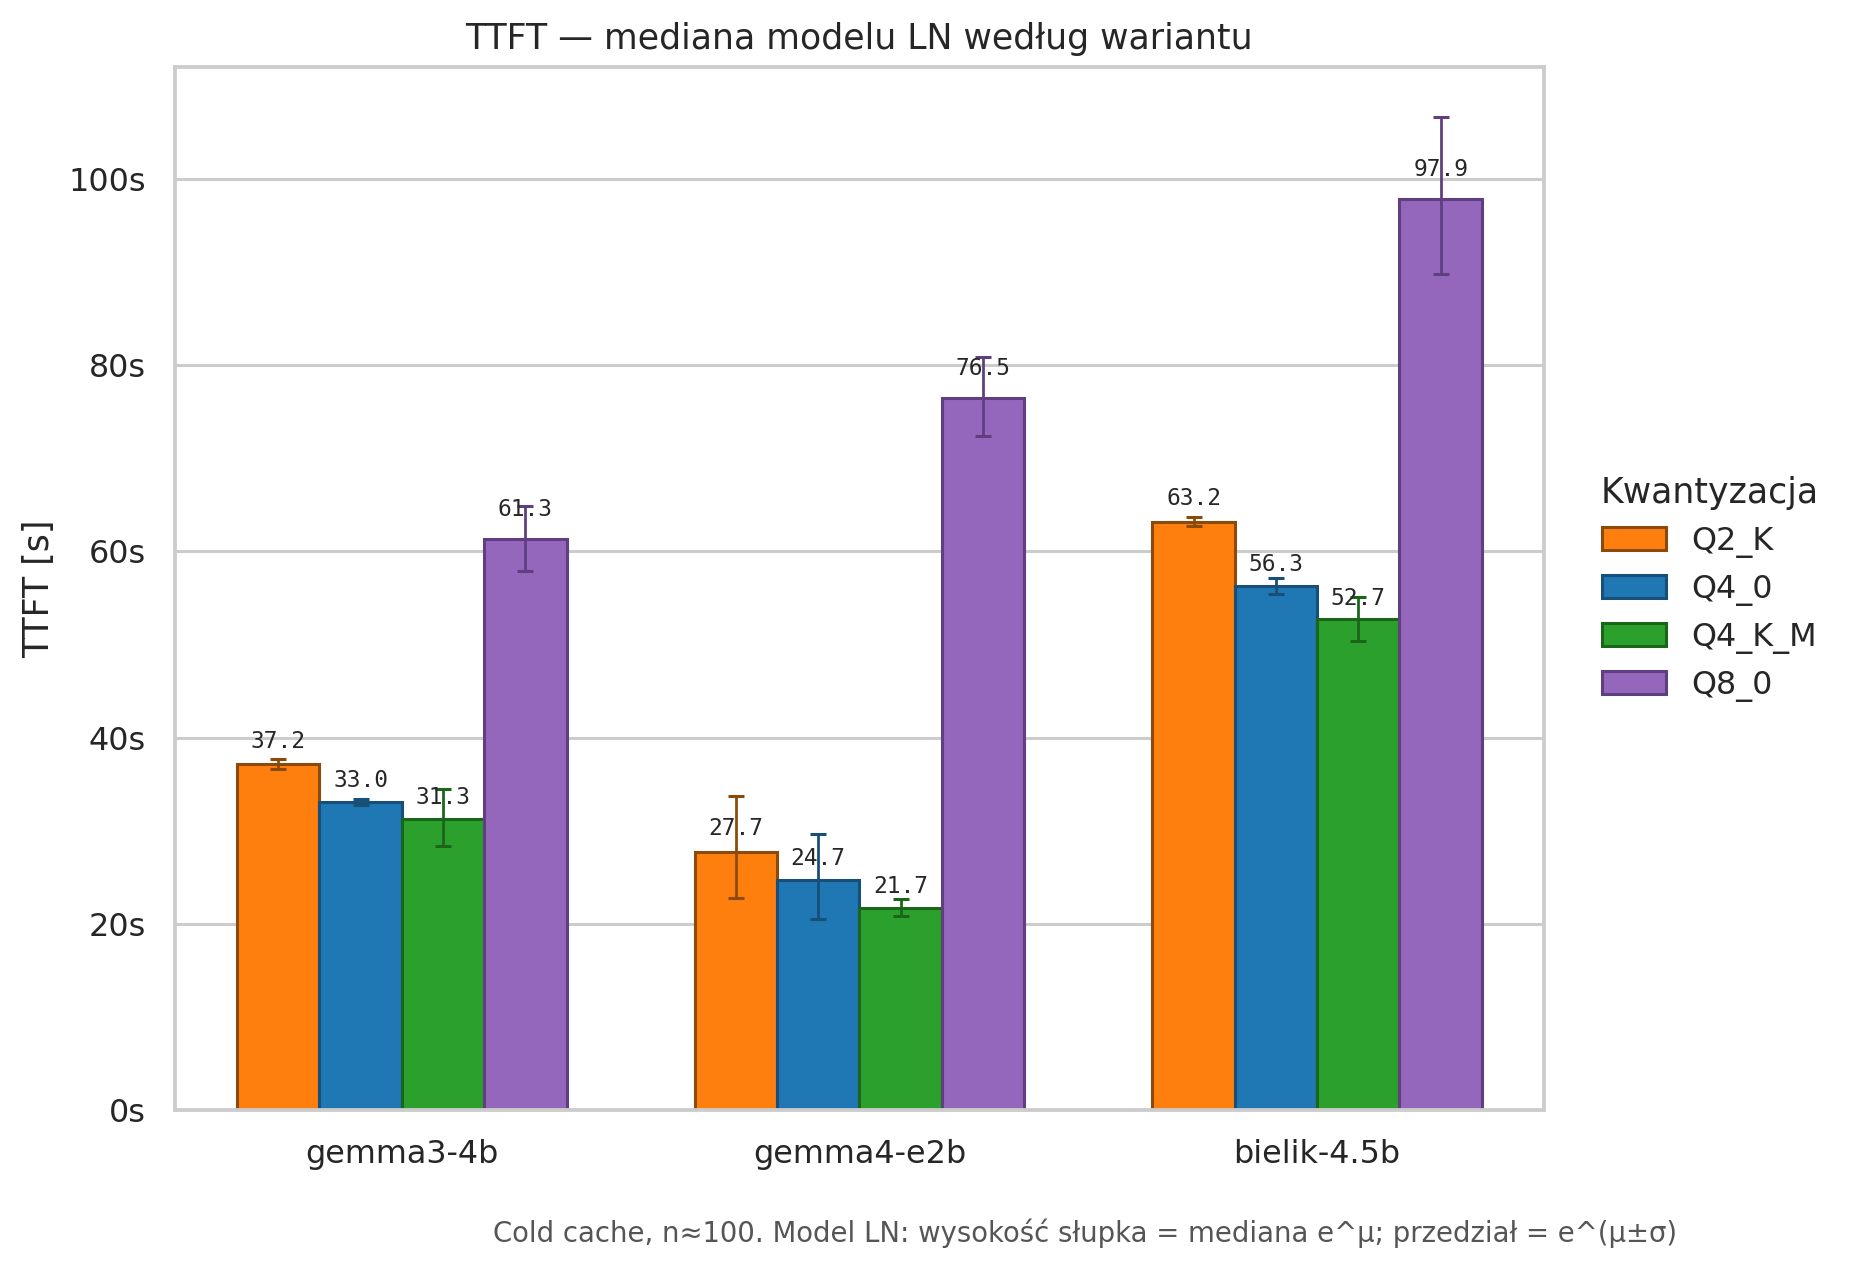
\includegraphics[width=0.85\textwidth]{cold_02_ttft_wedlug_wariantu.png}
  \caption{TTFT według wariantu kwantyzacji (cold cache):
           mediana modelu LN $e^{\hat\mu}$ z~przedziałem $e^{\hat\mu\pm\hat\sigma}$.}
  \label{fig:cold_ttft}
\end{figure}

\begin{figure}[H]
  \centering
  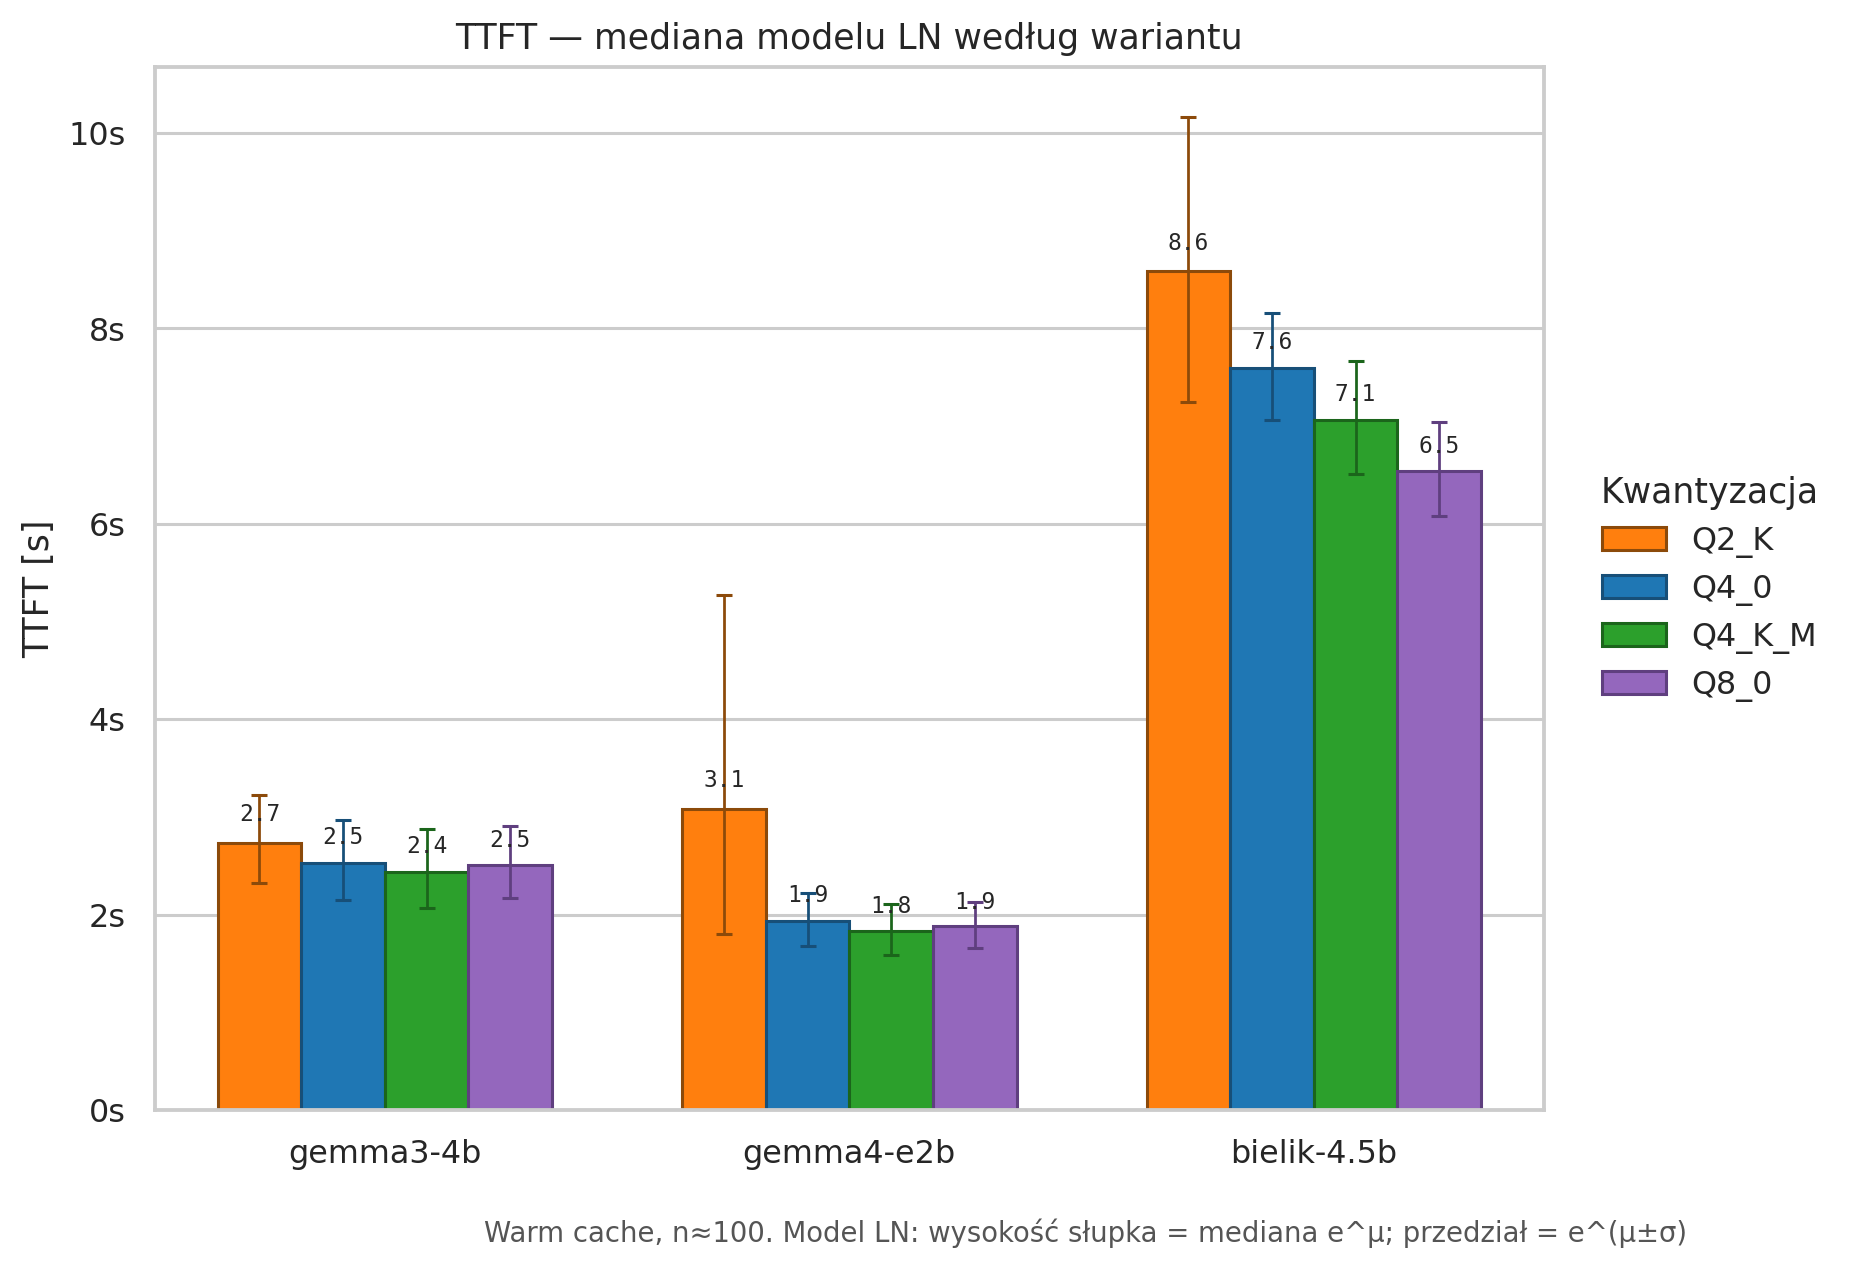
\includegraphics[width=0.85\textwidth]{02_ttft_wedlug_wariantu.png}
  \caption{TTFT według wariantu kwantyzacji (warm cache):
           mediana modelu LN $e^{\hat\mu}$ z~przedziałem $e^{\hat\mu\pm\hat\sigma}$.}
  \label{fig:ttft_warm}
\end{figure}

\subsubsection{Konsekwencje dla promptu Wilga}

Architektura promptu pod \emph{prefix caching}:
\begin{itemize}
  \item \textbf{[STATYCZNY PREFIKS]:} instrukcje, reguły (brak danych
        $\rightarrow$ przyznaj wprost), format odpowiedzi,
  \item \textbf{[DYNAMICZNY SUFIKS]:} dane sensoryczne, kontekst nauczyciela,
        pytanie użytkownika.
\end{itemize}
Po wdrożeniu \emph{prefix caching} i~kwantyzacji Q4\_K\_M dla
\texttt{gemma3-4b}: TTFT $\approx 2{,}4$~s, generacja $\approx 6{,}4$~s,
E2E $\approx 9$~s (mediany modelu LN, warm) --- akceptowalne dla asystenta
głosowego względem cold E2E rzędu kilkudziesięciu sekund.


% ============================================================
\subsection{Analiza wyników i rekomendacja produkcyjna}
\label{subsec:rekomendacja}
% ============================================================

\subsubsection{Porównanie modeli: wyniki końcowe}

Tabela~\ref{tab:wyniki_finalne} zestawia wyniki Optuny
(\texttt{results-selected-9.05}) z~95\%-owymi przedziałami ufności score
i~halucynacji (bootstrap) oraz średnim E2E~$\pm\sigma$ (model Gaussa).

\begin{table}[H]
  \centering
  \caption{Wyniki końcowe modeli z~przedziałami ufności 95\% (score, hal.)
           oraz średnim E2E~$\pm\sigma$ (\texttt{results-selected-9.05}).}
  \label{tab:wyniki_finalne}
  \small
  \begin{tabular}{lccccc}
    \hline
    Model & Score & 95\% CI score & Hal. & 95\% CI hal. & E2E średnia~$\pm\sigma$ \\
    \hline
    \texttt{gemma3:4b}  & 0{,}884 & [0{,}872, 0{,}894] & 1{,}17\% & [0{,}50\%, 2{,}17\%] & $30{,}4\pm 7{,}6$~s \\
    \texttt{llama3.2:3b}& 0{,}732 & [0{,}683, 0{,}780] & 16{,}5\% & [11{,}5\%, 22{,}0\%] & $26{,}8\pm 6{,}3$~s \\
    \texttt{gemma2:2b}  & 0{,}732 & [0{,}702, 0{,}760] & 18{,}3\% & [15{,}3\%, 21{,}5\%] & $20{,}5\pm 5{,}2$~s \\
    \texttt{qwen2.5:3b} & 0{,}697 & [0{,}645, 0{,}746] & 20{,}5\% & [15{,}0\%, 26{,}0\%] & $29{,}4\pm 6{,}6$~s \\
    \hline
  \end{tabular}
\end{table}

\texttt{gemma3:4b} dominuje jakościowo: score o~ok.~0{,}15 wyższy niż drugi
model, przy ok.~14-krotnie niższym wskaźniku halucynacji. Przedziały ufności
score nie zachodzą na siebie.

\subsubsection{Rekomendowana konfiguracja}

\begin{itemize}
  \item \textbf{Model:} \texttt{gemma3:4b},
  \item \textbf{Kwantyzacja:} Q4\_K\_M (ok.~$1{,}50\times$ szybsza generacja
        vs Q8\_0 przy warm cache; mniejszy plik GGUF),
  \item \textbf{Hiperparametry:} rozsądny preset (Optuna nie różnicuje silnie
        jakości semantycznej),
  \item \textbf{Prompt:} statyczny prefiks pod \emph{prefix caching},
  \item \textbf{Budżet czasu (warm, LN):} TTFT $\approx 2{,}4$~s, generacja
        $\approx 6{,}4$~s, E2E $\approx 9$~s.
\end{itemize}
Ograniczenie: halucynacje w~\texttt{missing\_data} i~\texttt{stale\_data}
nie są rozwiązane przez Optunę, kwantyzację ani cache --- wymagają
fine-tuningu (sekcja~\ref{subsec:finetuning_plan}).


% ============================================================
\subsection{Plan fine-tuningu jako kolejny krok badawczy}
\label{subsec:finetuning_plan}
% ============================================================

Analiza Optuny wykazała, że halucynacje w~kategoriach \texttt{missing\_data}
i~\texttt{stale\_data} są własnością wag modelu, a~nie konfiguracji inferencji.
Żaden z~badanych mechanizmów ich nie redukuje: Optuna wyjaśnia wariancję score
głównie flagą halucynacji bez zmiany \emph{nonhall\_score}; kwantyzacja zmienia
prędkość generacji, nie semantykę; \emph{prefix caching} skraca TTFT, nie
zachowanie modelu.

Jedyną metodą redukcji halucynacji w~tych kategoriach jest modyfikacja wag
przez fine-tuning na przykładach docelowego zachowania. Planowany eksperyment:
\begin{itemize}
  \item \textbf{Dataset:} 400~przykładów w~formacie \texttt{messages}
        (system/user/assistant), pokrywających kategorie \texttt{factual\_status},
        \texttt{missing\_data}, \texttt{conflicting\_data}, \texttt{stale\_data}
        i~\texttt{paraphrase},
  \item \textbf{Metoda:} LoRA przez \texttt{mlx-lm} na MacBook~M4 (Apple Silicon),
  \item \textbf{Model bazowy:} \texttt{gemma3:4b} (rekomendacja produkcyjna).
\end{itemize}

Pytanie badawcze: czy fine-tuned model \emph{bez} explicit reguł w~system prompcie
wyprzedza model bazowy \emph{z} regułami na kategoriach \texttt{missing\_data}
i~\texttt{stale\_data}? Stabilność \emph{nonhall\_score} sugeruje, że instrukcje
promptowe mają marginalny wpływ na trudne scenariusze --- fine-tuning adresuje
ten deficyt bezpośrednio.

Status: planowane --- wyniki poza zakresem czasowym niniejszej pracy.
Wnioski z~obecnych badań stanowią empiryczne uzasadnienie dla tego etapu.

\newpage
\section{Realizacja prototypu}
\label{sec:realizacja}

\subsection{Architektura prototypu}
\label{subsec:architektura_prototypu}

Zaimplementowany finalny system asystenta głosowego Wilga odpowiada oparty jest na koncepcji
z~rozdziału~\ref{subsec:przeplyw}, składają się na nią: aplikacja użytkownika, serwer orkiestrujący
oraz węzeł brzegowy Raspberry~Pi~5. Schemat wdrożenia przedstawiono
na rysunku~\ref{fig:architektura}, zastosowano ten sam podział na trzy
środowiska co na rysunku schematu testowego~\ref{fig:schemat}, w przypadku prezentowanej wdrożeniowej wersji asystenta przedstawiono architekturą wraz z~konkretnymi procesami i~kierunkami przepływu danych.

\begin{figure}[H]
    \centering
    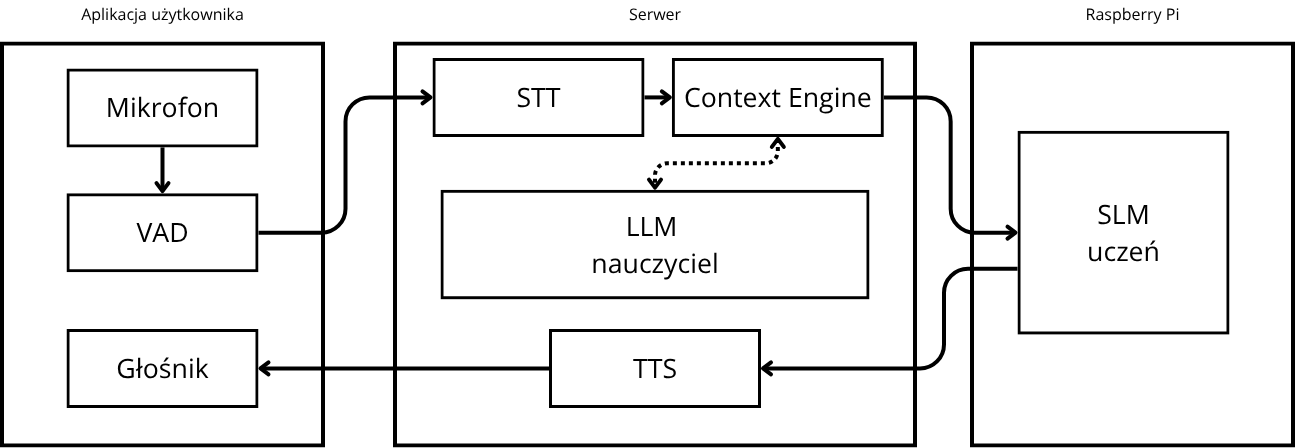
\includegraphics[width=\textwidth]{src/img/system-schemat.png}
    \caption{Architektura prototypu Wilga --- przepływ danych od mikrofonu
             do głośnika. Linia przerywana oznacza asynchroniczną współpracę
             Context Engine z~modelem Nauczyciela.}
    \label{fig:architektura}
\end{figure}

Architektura produkcyjna jest pokrewna, lecz nie tożsama z~układem
benchmarkowym opisamym w sekcji~\ref{subsec:metodologia} (rysunek~\ref{fig:testy_arch}).
Wspólnym elementem pozostaje gówny aktor: węzeł brzegowy, na który składają się serwer Ollama oraz mały model
językowy (SLM) Uczeń na Raspberry~Pi~5. Względem architektury testowej największe zmiany poczyniono w warstwie serwerowej.
W~pomiarach orkiestratorem był skrypt testowy oraz złoty zbiór pytań (\emph{golden set}); w~prototypie tę rolę przejmuje pełny łańcuch
głosowy (aktywowany przez użytkownika) oraz Context Engine (działający asynchronicznie). Konfiguracja modelu Ucznia
pochodzi z~rekomendacji badawczej (tabela~\ref{tab:rekomendacja_produkcyjna}), wybrano \texttt{gemma3:4b}, kwantyzacja Q4\_K\_M, \texttt{keep\_alive=30m}
oraz stały prefiks promptu pod \emph{prefix caching}.

Przepływ danych wywołany zapytaniem użytkownika przebiega wzdłuż strzałek
na rysunku~\ref{fig:architektura}. Mikrofon przez przeglądarkę rejestruje
sygnał audio. Detekcja aktywności mowy (ang.\ \emph{Voice Activity Detection},
VAD) w~aplikacji kończy nagranie po chwili ciszy; start następuje po wywołaniu frazy
\textit{,,Hej Wilguś''} albo po kliknięciu postaci na ekranie. Segment audio trafia
na serwer, gdzie transkrypcja (ang.\ \emph{Speech-to-Text}, STT) zamienia
mowę na tekst. Context Engine dokłada do pytania stały prefiks reguł, dane z~czujników oraz bieżący kontekst wygenerowany przez Nauczyciela. Tak złożone żądanie trafia  na urządzenie brzegowe Raspberry~Pi, do modelu SLM Ucznia. Wygenerowana odpowiedź wraca na serwer, synteza
mowy (ang.\ \emph{Text-to-Speech}, TTS) produkuje audio, które jest transportowane do aplikacji użytkownika gdzie głośnik
 odtwarza odpowiedź.

Context Engine nie stoi na ścieżce krytycznej zapytania. Pracuje w~dwóch
cyklach. Cykl asynchroniczny, sterowany interwałem
\texttt{CONTEXT\_REFRESH\_INTERVAL} (domyślnie 300~s), w~tle przesuwa
kursor po historycznych odczytach IoT (rekordy bazy danych), odpytuje Nauczyciela i buduje konktest na bieżąco. Całość odvywa się przy pomocy skryptów w~języku Python w sposób cykliczny i asynchroniczny, niezależnie od użytkownika. Cykl synchroniczny skupia się jedynie na doklejeniu aktualnego kontekstu do pytania użytkownika oraz przed przesłaniem zapytania do modelu Ucznia. Czas odpowiedzi asystenta nie zależy więc od czasu generacji
Nauczyciela. Linia przerywana na schemacie oznacza właśnie tę asynchroniczną,
dwukierunkową współpracę silnika kontekstu modelem LLM.

Podział maszyn jest zgodny z~założeniem o~odciążeniu urządzenia brzegowego.
Komputer Mac (serwer) wykonuje transkrypcję, syntezę mowy, budowanie
kontekstu i~inferencję Nauczyciela. Raspberry~Pi udostępnia wyłącznie
interfejs Ollama API, tak aby całe zasoby były przeznaczone dla modelu SLM.

\subsection{Elementy systemu i wykorzystane technologie}
\label{subsec:elementy}

W poniższej sekcji skupiono się na kolejnych elementach systemu, ich roli oraz wykorzystanych technologiach.

\subsubsection{Aplikacja użytkownika}

Interfejs użytkownika zrealizowano w~React z~wykorzystaniem bundlera Vite, za część stylistyczną odpowiada Tailwind CSS.
Aplikacja nie transkrybuje mowy ani nie syntetyzuje odpowiedzi. Jej zadania ograniczają się do:
nagrania audio, wyświetlania historię rozmowy oraz wizualinych zmian stanów, takich jak animacja maskotki Wilguś. Wiele wyborów technologicznych dotyczących tej warstwy wynikało z dziedziczenia koncepcji architektonicznych poprzedniej aplikacji Wilga MiLL, co 
opisano w rozdziale~\ref{sec:koncepcja}.

System obsługuje dwa tryby aktywacji. W~trybie głosowym przeglądarka
nasłuchuje frazy kluczowej \textit{,,Hej Wilguś''} przez Web Speech API
(Chrome/Edge). Rozpoznawane są także warianty transkrypcji (obsługa błędów)
(\texttt{hej wilga}, \texttt{hej wilgo}, \texttt{hey wilgus} i~podobne);
po wykreyciu frazy kluczowej frontend obcina frazę z~początku wypowiedzi, żeby asystent
nie traktował jej jako pytania, jest ona jedynie wywołaniem systemu. W~trybie ręcznym nagranie startowane jest poprzez
kliknięciem postaci Wilgusia na ekranie. W~obu przypadkach ten sam odcinek jest nagrywany i przesyłany do sytemu.

Mechanizm znalezienia momentu, w którym nagrywanie zostaje wstrzymane oparto o~prosty detektor poziomu głośności badany przez mikrofon urządzenia końcowego, a~nie o~model Silero omawiany w~przeglądzie
literatury. Utrzymanie się poniżej wyznaczonego progu przez 1{,}5~s kończy nagranie;
dolny i~górny limit trwania to 2{,}5~s oraz 20~s. Rozwiązanie jest
lżejsze niż neuronowy VAD i w testach wykazało, że dobrze sprawdza się do naturalnego ucięcia wypowiedzi
bez instalowania dodatkowego modelu na serwerze. Wyznaczenie końca nagrania nie jest zatem adaptacyjne. Poziom, który uznano za ciszę jest stałą w kodzie aplikacji. W domkach w Wildze, które znajdują się w lesie panują dość dobre warunki akustyczne. Niemniej dobrym kierunkiem rozwoju byłoby adaptacyjne ustawienie progu lub filtrowanie częstotliwości zbieranych prze mikrofon.

Układ interfejsu użytkownika jest dwukolumnowy. Po lewej stronie znajduje się karta \emph{Rozmowa} gdzie wyświetlany jest czat, po prawej widneje postać Wilgusia (animowana w zależności od statusu). Aplikacja na starcie po uruchomieniu, przechodzi przez fazę przygotowawczą. Zanim użytkownik może zadać pierwsze pytanie, model Uczeń musi być przygotowany, fazę tę nazwano rozgrzeaniem. Faza ta ma zapobiegać wydłużonej odpowiedzi na pierwsze zapytanie, które
trafioby w~\emph{cold cache} i~czas do pierwszego tokenu (TTFT) sięgałby rzędu dziesiątek sekund, tal jak wykazano to w ~sekcji~\ref{subsec:kwantyzacja}.
Pętla \texttt{StudentKeepWarm} razem z~\texttt{keep\_alive} ustawionym
na 30~min powodują, że zarówno wagi modelu jak i~KV-cache stałego prefiksu ciągle znajduje się w~RAM
urządzenia brzegowego co zapobiega jego ładowania do pamięci podręcznej w momencie pojawienia się zapytania użytkownika.
Frontend odpytuje endpoinu \texttt{GET /api/health}, który w czasie rozgrzewania modelu zwraca status \texttt{warming} co blokuje interakcję użytkownika.
Widok prezentowany userowi podczas fazy przygotowawczej przedstawiono na rysunku~\ref{fig:app_warmup}.

\begin{figure}[H]
    \centering
    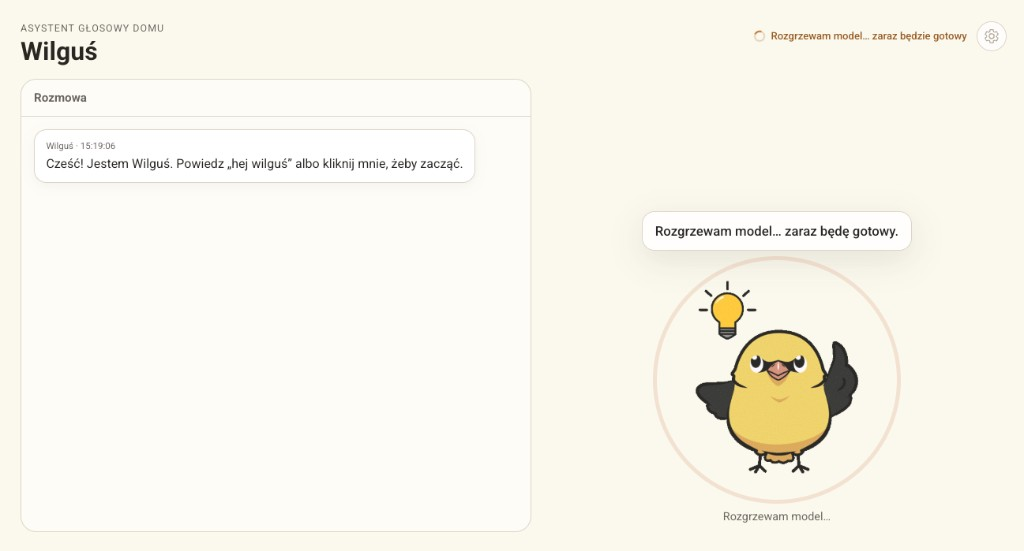
\includegraphics[width=\textwidth]{src/img/app_warmup.png}
    \caption{Faza rozgrzewania modelu Ucznia. Interfejs informuje
             o~ładowaniu wag i~KV-cache, zanim możliwe będzie zapytanie
             bez kosztu \emph{cold cache}.}
    \label{fig:app_warmup}
\end{figure}

Po zakończeniu procesu rozgrzewania modelu Ucznia użytkownikowi prezentowany jest delikatnie inny widok-  ekran startowy
(rysunek~\ref{fig:app_start}): powitanie, subtelne instrukcje jak rozpocząć rozmowę (raza startowa lub kliknięcie Wilgusia). Dodatkow aby zachęcić do interakcji postać Wilgusi pulsuje pokazując swoją gotowość do interakcji. Widok startowy nadal trzyma omówiony powyżej dwukolumnowy układ.

\begin{figure}[H]
    \centering
    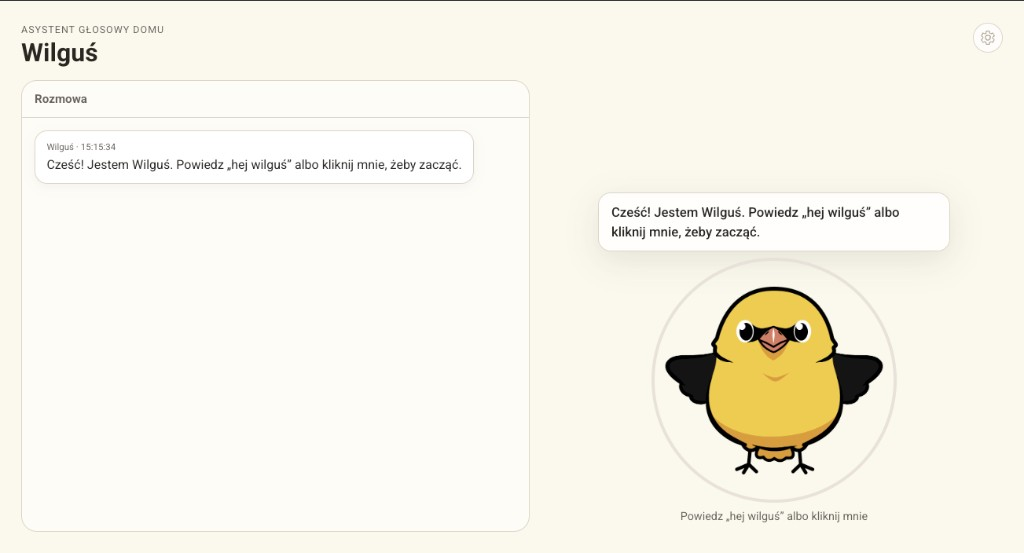
\includegraphics[width=\textwidth]{src/img/app_start.png}
    \caption{Ekran startowy po rozgrzaniu modelu: karta historii rozmowy
             oraz interaktywna postać Wilguś.}
    \label{fig:app_start}
\end{figure}

Wilguś widoczny w prawej kolumnie prezentowanych widoków nie jest statyczną ilustracją. Tablica \texttt{WILGUS\_BY\_STATUS}
przypisuje fazom czy statusom aplikacji osobną grafikę dynamiczną i~podpis, dzięki czemu postać
sygnalizuje, co system właśnie robi. Grafiki zapisane w formacie GIF wprowadzają element ruchu, który podnosi zaangażowanie użytkownika. Klatki faz używanych w~prototypie
zestawiono na rysunku~\ref{fig:wilgus_fazy}. Postać Wilgusia została zaprojektowana przez Julię Nazarską, studentkę wydziały Architektury Politechniki Warszawskiej.

\begin{figure}[H]
    \centering
    \begin{minipage}[t]{0.18\textwidth}
        \centering
        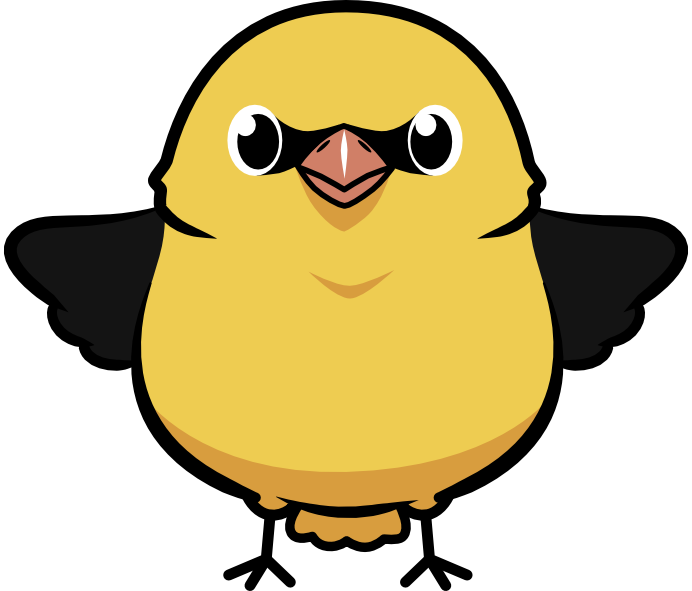
\includegraphics[width=\linewidth]{src/img/wilgus/wilgus_neutral.png}\\[0.4em]
        {\small gotowy / \textit{hej wilguś}}
    \end{minipage}
    \hfill
    \begin{minipage}[t]{0.18\textwidth}
        \centering
        
\includegraphics[width=\linewidth]{src/img/wilgus/wilgus_macha.png}\\[0.4em]
        {\small słucham dalej}
    \end{minipage}
    \hfill
    \begin{minipage}[t]{0.18\textwidth}
        \centering
        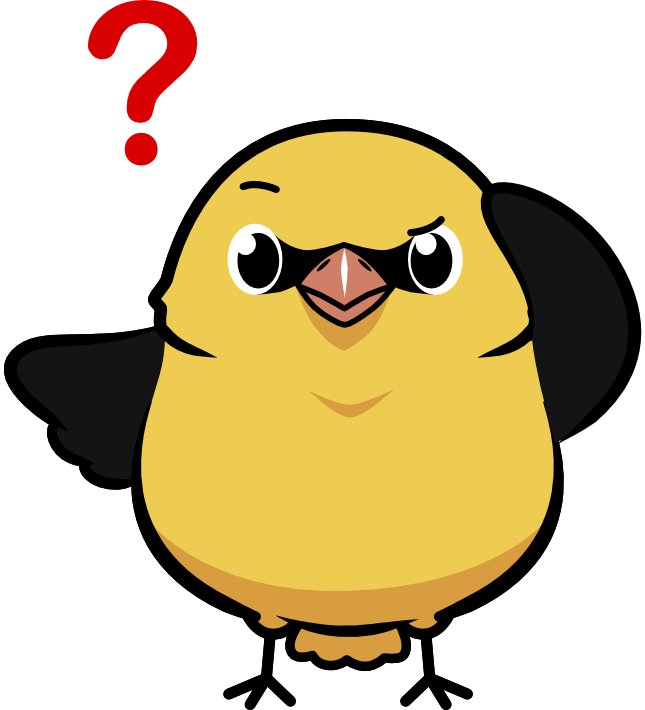
\includegraphics[width=\linewidth]{src/img/wilgus/wilgus_zdziwiony.png}\\[0.4em]
        {\small nagrywam}
    \end{minipage}
    \hfill
    \begin{minipage}[t]{0.18\textwidth}
        \centering
        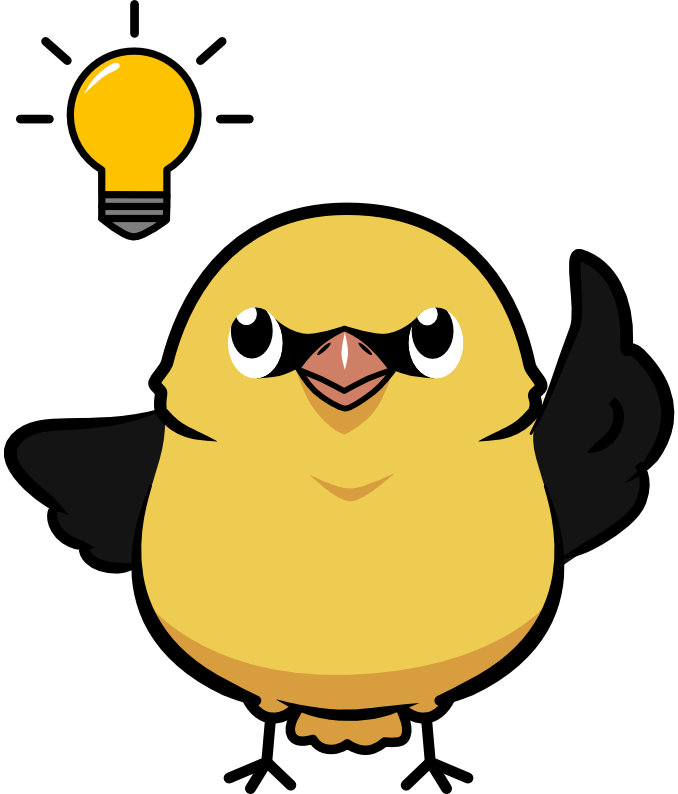
\includegraphics[width=\linewidth]{src/img/wilgus/wilgus_pomysl.png}\\[0.4em]
        {\small myślę}
    \end{minipage}
    \hfill
    \begin{minipage}[t]{0.18\textwidth}
        \centering
        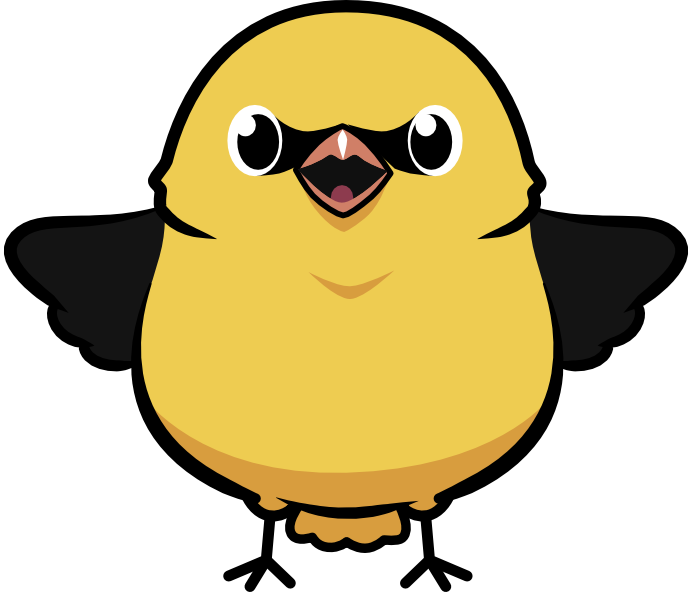
\includegraphics[width=\linewidth]{src/img/wilgus/wilgus_gada.png}\\[0.4em]
        {\small mówię}
    \end{minipage}
    \caption{Stany Wilgusia w aplikacji użytkownika.}
    \label{fig:wilgus_fazy}
\end{figure}

Podczas konwersacji lewa kolumna wypełnia się wiadomościami użytkownika i odpowiedziami asystenta. Całość ma przypominać dobrze znany interfejs chatu, przez co korzystanie z aplikacji jest intuicyjne. Na rysunku~\ref{fig:app_rozmowa} przedstawiono przykładowy widok w trakcie prowadzenia rozmowy.

\begin{figure}[H]
    \centering
    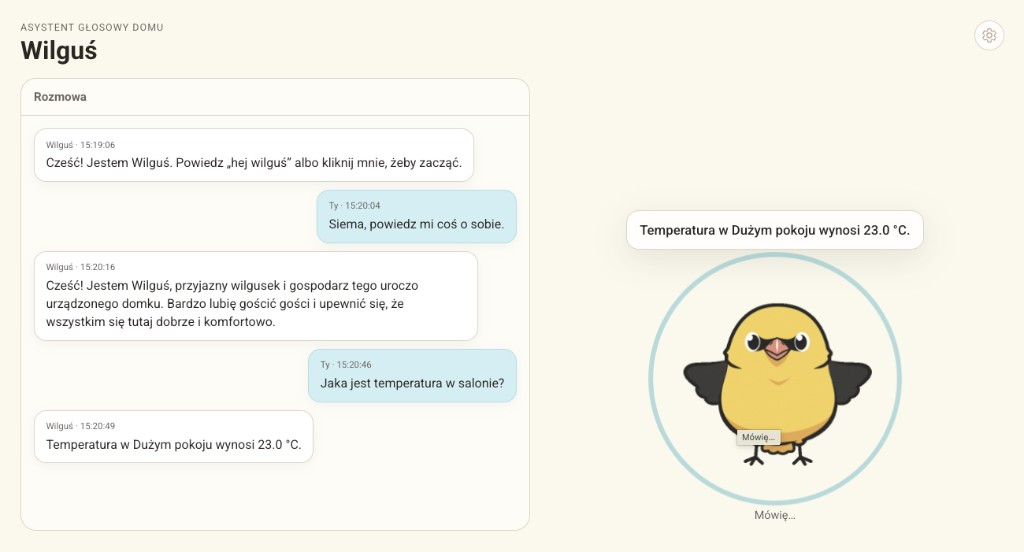
\includegraphics[width=\textwidth]{src/img/app_rozmowa.png}
    \caption{Widok aplikacji w trakcie prowadzenia rozmowy.}
    \label{fig:app_rozmowa}
\end{figure}

\subsubsection{Transkrypcja mowy (STT)}

Za transkrypcję mowy, czyli element procesu nazwany STT na schemacie architektonicznym (rysunek~\ref{fig:architektura}) odpowiada blok roboczo nazwany Whisper Backend. Jest to usługa stworzono w oparciu o bliblitekę języka Python FastAPI oraz otwartoźródłowego modelu Whisper. Sercem moduły jest transkrypcja, którą realizuje biblioteka \texttt{faster-whisper} \cite{Radford2023}. W prezentowanym rozwiązaniu zdecydowano się implementować wa
wariant \texttt{small}, oczywiście w konfiguracji wskazano język polski (\texttt{pl}). Filtr VAD po stronie Whisper jest wyłączony
(\texttt{WHISPER\_VAD\_FILTER=false}), ponieważ w systemie istnieje własny detektor aktywności, widoczny na schemacie architektornicznym pod nazwa \texttt{VAD}.

Nagranie zebrane przez aplikację użytkownika zostaje wysłane do Whisper Backendu poprzez żądanie HTTP \texttt{POST /api/transcribe},
pole \texttt{file}) zawiera plik nagrania (mechanizm znany z formularzy aplikacji webowych \texttt{multipart/form-data})). Odpowiedź zwracana jest w formacie JSON, jej przykład przedstawiono poniżej:

\begin{verbatim}
{"text": "jaka jest temperatura w salonie",
 "language": "pl",
 "duration_seconds": 2.4}
\end{verbatim}

Moduł STT został zabezpieczony przez błedami. Serwis odrzuca nagrania większe niż 25~MB oraz niemal puste pliki
(poniżej ok.\ 1{,}5~kB), brak reakcji na szum. 

\subsubsection{Context Engine}
\label{subsec:kontekst}

Context Engine jest zestawem skryptów Python opakowanych w~FastAPI
na porcie \texttt{8001}. Ponieważ instalacja IoT w~Wildze nie dostarczała
strumienia na żywo w~trakcie prac, serwis czyta historyczny CSV
z~\texttt{db\_sampler} (okres 31.10.2025--27.01.2026, 147~kolumn
wraz z~polem czasu).
Każdy cykl odświeżania przesuwa kursor o~jeden wiersz (w~danych jest to
krok ok.~5~minut); po ostatnim wierszu symulacja wraca na początek.
Do promptu nie idzie pełna szerokość tabeli --- parser zostawia metryki
komfortu i~stanu technicznego (temperatura, wilgotność, obecność,
kontaktrony, oświetlenie, moc, energia, VOC) i~pomija m.in.\ baterie
oraz jakość łącza, żeby nie rozdymać okna kontekstu Ucznia.

Fakty dla Ucznia składa warstwa deterministyczna: z~wiersza CSV powstaje
punktowy \emph{snapshot} z~etykietami pomieszczeń (łazienka, duży pokój,
mały pokój, korytarz). Model językowy nie liczy progów ani stanów
boolowskich. Nauczyciel dostaje ten sam snapshot wyłącznie po to,
by zgłosić anomalie. Jeśli wywołanie się nie uda, fakty i~tak zostają
opublikowane --- serwis nie blokuje asystenta na awarii większego modelu.

Kontekst ma dwa bufory. \emph{Published} jest przypięty do bieżącej
rozmowy; \emph{staging} odświeża się w~tle. Nowa sesja
(\texttt{POST /api/session/new} po stronie Whisper Backendu) woła
\texttt{POST /api/context/advance} i~przestawia publikowany snapshot
na nowszy, bez zmiany stałego prefiksu reguł. Dzięki temu KV-cache
prefiksu na Pi pozostaje ważny między turami.

Whisper Backend pobiera bieżący kontekst przez
\texttt{GET /api/context}. Przykładowa odpowiedź:

\begin{verbatim}
{
  "status": "ready",
  "source_timestamp": "2025-11-01T12:00:00Z",
  "static_prefix": "Jesteś Wilguś — ...",
  "dynamic_context": "Stan mieszkania na ... UTC: ...",
  "system_prompt": "Jesteś Wilguś — ...\n\nStan mieszkania...",
  "insight": "Okno w korytarzu otwarte."
}
\end{verbatim}

Pole \texttt{static\_prefix} (persona i~reguły) jest niezmienne między
zapytaniami. Pole \texttt{dynamic\_context} to fakty plus opcjonalna
sekcja Findings. Pole \texttt{system\_prompt} jest złożeniem obu części,
zostawionym dla zgodności wstecznej. Przy \texttt{status: pending}
(pierwszy cykl po starcie) backend nie czeka w~nieskończoność:
używa zapasowego prefiksu wbudowanego w~Whisper Backend i~może
odpowiadać bez faktów, zamiast blokować cały interfejs.

\subsubsection{LLM Nauczyciel}

Nauczyciel działa lokalnie na Macu przez Ollamę
(adres w~\texttt{TEACHER\_OLLAMA\_URL}, model \texttt{qwen2.5}),
z~\texttt{keep\_alive} równym 30~min i~bez strumieniowania. Zadanie jest wąskie:
nie streszczać całego domu, tylko wskazać odchylenia (skrajne temperatury,
otwarte okna, nietypowa obecność, wysokie VOC, sprzeczne odczyty).
Gdy nic nie zasługuje na uwagę, model ma zwrócić dokładnie jedną linię
\texttt{BRAK\_ANOMALII}; serwis traktuje to jako brak findings
i~nie dokleja sekcji do promptu Ucznia.

Żądanie do Ollamy ma postać:

\begin{verbatim}
{
  "model": "qwen2.5",
  "messages": [
    {"role": "system", "content": "Jesteś analitykiem IoT smart-home..."},
    {"role": "user",   "content": "Snapshot czujników z ..."}
  ],
  "stream": false,
  "keep_alive": "30m"
}
\end{verbatim}

\subsubsection{SLM Uczeń}

Uczeń to \texttt{gemma3:4b} na Raspberry~Pi (Ollama API w~sieci lokalnej),
w~konfiguracji z~tabeli~\ref{tab:rekomendacja_produkcyjna}. Zapytanie
z~frontendu to \texttt{POST /api/chat}:

\begin{verbatim}
{
  "message": "Jaka jest temperatura w salonie?",
  "history": [
    {"role": "user", "content": "Siema, powiedz mi coś o sobie"},
    {"role": "assistant", "content": "Jestem Wilguś, gospodarz domku..."}
  ]
}
\end{verbatim}

Backend dokłada co najwyżej ostatnie sześć tur historii
(\texttt{CHAT\_HISTORY\_MAX\_MESSAGES}). Payload do Ollamy rozdziela
role tak, by prefiks systemowy był bitowo stały: najpierw
\texttt{role: system} ze \texttt{static\_prefix}, potem --- jeśli są ---
fakty domu jako osobna wiadomość użytkownika, następnie historia
i~bieżące pytanie. Włączenie \texttt{stream: true} oraz
\texttt{keep\_alive} z~konfiguracji pozwala strumieniować tokeny
i~utrzymać ciepły cache. Odpowiedź do przeglądarki idzie jako NDJSON:

\begin{verbatim}
{"type":"chunk","content":"Temperatura w Dużym pokoju"}
{"type":"chunk","content":" wynosi 23,0 °C."}
{"type":"done"}
\end{verbatim}

Zdarzenie \texttt{error} pojawia się przy przekroczeniu limitu czasu
Ollamy (120~s, HTTP~504 na etapie połączenia) albo przy błędzie sieci.
Gdy Context Service nie odpowiada, Uczeń dostaje wyłącznie zapasowy
prefiks persony i~odmawia cytowania liczb spoza faktów --- zgodnie
z~regułami promptu.

\subsubsection{Synteza mowy (TTS)}

Frontend tnie napływające zdania i~kolejkuje
\texttt{POST /api/tts} z~ciałem \texttt{\{"text": "..."\}}.
Odpowiedź to \texttt{audio/mpeg}. Syntezę realizuje \texttt{edge-tts}
\cite{EdgeTTS} głosem \texttt{pl-PL-ZofiaNeural}; wymaga to sieci
wychodzącej do usług Microsoft. Limit długości wynosi 1000~znaków.
Takie podejście daje akceptowalną jakość polszczyzny bez trenowania
własnego TTS, przy czym sam Uczeń nadal liczy się wyłącznie lokalnie.

\subsubsection{Konfiguracja}

Adresy, nazwy modeli i~interwały siedzą w~plikach \texttt{.env},
bez zmian w~kodzie:

\begin{itemize}
    \item \texttt{context\_service/.env}: \texttt{TEACHER\_OLLAMA\_URL},
          \texttt{TEACHER\_OLLAMA\_MODEL}, \texttt{CONTEXT\_REFRESH\_INTERVAL},
          \texttt{SENSOR\_DATA\_PATH};
    \item \texttt{whisper-proj/backend/.env}: \texttt{OLLAMA\_URL},
          \texttt{OLLAMA\_MODEL}, \texttt{CONTEXT\_SERVICE\_URL},
          \texttt{WHISPER\_MODEL\_SIZE}, \texttt{OLLAMA\_KEEP\_ALIVE},
          \texttt{TTS\_VOICE}.
\end{itemize}

\subsection{Testy rozwiązania}
\label{subsec:testy_prototypu}

Pełny stos uruchamia skrypt \texttt{start.sh}: lokalna Ollama Nauczyciela,
Context Service, Whisper Backend i~serwer deweloperski frontendu.
Przed startem skrypt sprawdza \texttt{/api/tags} obu instancji Ollamy,
obecność modeli oraz środowiska Python; Nauczyciela rozgrzewa od razu,
Ucznia --- pętla keep-warm w~backendzie, ta sama która steruje
rysunkiem~\ref{fig:app_warmup}.

Odporność na typowe awarie wbudowano w~ścieżkę żądania, a~nie w~osobny
moduł. Brak pierwszego snapshotu zgłasza \texttt{status: pending};
niedostępny Context Service spada na zapasowy prefiks; pad Nauczyciela
zostawia fakty bez Findings; rozgrzewający się Uczeń wraca 503;
przekroczenie czasu Ollamy --- 504. Interwał keep-warm (10~min) jest
krótszy niż \texttt{keep\_alive} (30~min), żeby model nie wypadł
z~pamięci między turami.

Poprawność łańcucha sprawdzano ręcznie: uruchomienie aplikacji
i~rozmowy głosowe oraz tekstowe, w~scenariuszach zbliżonych do złotego
zbioru z~części badawczej --- pytanie o~stan (temperatura, oświetlenie),
brak danych (oczekiwana odmowa zamiast halucynacji) oraz nieaktualny
znacznik czasu. W~pracy tekstowej nie zamieszcza się nagrań sesji;
zrzuty na rysunkach~\ref{fig:app_start}--\ref{fig:app_rozmowa} dokumentują
układ i~przykładową turę, nie pełną ewaluację jakości.

Czasy odpowiedzi w~prototypie mieszczą się w~rzędzie wielkości
zmierzonych dla konfiguracji produkcyjnej: przy \emph{warm cache}
mediana E2E modelu LN wynosi ok.~9~s
(tabela~\ref{tab:rekomendacja_produkcyjna}). Bez rozgrzania i~stałego
prefiksu ten sam węzeł wraca do opóźnień cold-cache omówionych
w~sekcji~\ref{subsec:kwantyzacja}.

\newpage
\section{Podsumowanie}

\subsection{Wnioski z przeprowadzonych badań}

Część badawcza (rozdział~\ref{sec:modele}) przebiegała jako sekwencja czterech
kolejnych odkryć, z~których każde ukierunkowywało następny eksperyment. Uzyskane
wyniki pozwoliły sformułować pięć wniosków, które łącznie potwierdzają, że
uruchomienie użytecznego asystenta głosowego opartego na małym modelu językowym
(SLM) na urządzeniu brzegowym klasy Raspberry~Pi~5 jest wykonalne.

Po pierwsze, stabilność termiczna platformy brzegowej okazała się warunkiem
koniecznym wiarygodnego pomiaru. Instalacja aktywnego chłodzenia sterowanego
GPIO zredukowała udział dławienia termicznego ze~100\% (Run~1) do~0\% (Run~2),
dzięki czemu ranking modeli przestał odzwierciedlać odporność na throttling,
a~zaczął mierzyć jakość semantyczną. Model docelowy \texttt{gemma3:4b} awansował
z~czwartego na pierwsze miejsce: \emph{composite score} wzrósł z~0{,}497 do~0{,}806
($+62{,}3\%$), a~mediana E2E skróciła się z~57\,584~ms do~31\,742~ms
($1{,}81\times$ szybciej) --- por.~tabele~\ref{tab:ranking_run1}
i~\ref{tab:ranking_run2}.

Po drugie, analiza statystyczna Run~3 wykazała, że o~wyniku decyduje przede
wszystkim flaga halucynacji: sama \texttt{hallucination\_flag} wyjaśnia
$R^2 = 0{,}9922$ wariancji \emph{composite score}, podczas gdy hiperparametry
inferencji zaledwie $R^2 = 0{,}2997$ (rysunek~\ref{fig:regression_r2}). Wniosek
ten jest pozytywny w~sensie metodologicznym: badanie precyzyjnie zlokalizowało
właściwą dźwignię optymalizacji, wskazując, że wysiłek należy kierować na wybór
modelu i~modyfikację jego wag, a~nie na strojenie parametrów generacji.

Po trzecie, kwantyzacja wag okazała się skuteczną i~bezpieczną metodą
przyspieszenia generacji. Zaprojektowana metodyka \emph{warm-cache} pozwoliła
wyizolować \emph{generation\_ms} spod maskującego wpływu prefill (TTFT)
i~zmierzyć rzeczywisty efekt precyzji wag. Wariant Q4\_K\_M zapewnił
$1{,}46\times$ przyspieszenie generacji dla \texttt{gemma3-4b} i~$1{,}67\times$
dla \texttt{gemma4-e2b} względem pełnej precyzji Q8\_0, przy jednoczesnym
zmniejszeniu pliku GGUF o~ok.~40\% i~bez degradacji jakości semantycznej
(tabela~\ref{tab:kwantyzacja_wyniki}). Q4\_K\_M jest zatem optymalnym
kompromisem między rozmiarem, szybkością a~jakością dla modeli rodziny Gemma.

Po czwarte, i~jest to wynik kluczowy dla użyteczności prototypu, udało się
radykalnie zredukować czas do pierwszego tokenu (TTFT). Na Raspberry~Pi~5
pracującym wyłącznie na procesorze (CPU-only) prefill długiego promptu
systemowego dominuje całkowite opóźnienie --- przy zimnym cache TTFT stanowi
ok.~87\% E2E. Utrzymanie modelu oraz pamięci podręcznej kluczy i~wartości
(KV-cache) w~,,ciepłej'' pamięci RAM (\texttt{keep\_alive=30m}) w~połączeniu
z~konstrukcją promptu ze stałym prefiksem (\emph{prefix caching}) skróciło
medianę TTFT z~ok.~27\,387~ms do~ok.~2378~ms, co odpowiada redukcji rzędu
91\% (ostrożnie szacowanej na ok.~84\% w~warunkach produkcyjnych). Ponieważ
urządzenie brzegowe nie dysponuje akceleratorem GPU, to właśnie zachowanie
gorącego stanu w~RAM eliminuje najkosztowniejszy etap i~czyni interaktywnego
asystenta głosowego na CPU-only realnym.

Po piąte, połączenie powyższych dźwigni prowadzi do konkretnej, rekomendowanej
konfiguracji produkcyjnej: \texttt{gemma3:4b} z~kwantyzacją Q4\_K\_M
i~\emph{prefix cachingiem}. Osiąga ona E2E na poziomie ok.~8{,}3~s przy
wskaźniku halucynacji 1{,}17\% --- czternastokrotnie niższym niż druga
najlepsza opcja (16{,}5\%), przy czym różnice są istotne statystycznie
(rozłączne przedziały ufności~95\%, tabela~\ref{tab:wyniki_finalne}).

\subsection{Ocena prototypu względem założeń}

Tezę pracy sformułowano w~dwóch wymiarach (sekcja~\ref{sec:modele} oraz wstęp),
które posłużą tutaj jako punkt odniesienia dla oceny prototypu.

Pierwszy wymiar --- zwiększenie dostępności informacji o~stanie domku
wypoczynkowego dla użytkownika nietechnicznego poprzez lokalny interfejs
głosowy --- został zrealizowany. Zbudowany prototyp o~architekturze
Teacher--Student działa w~kompletnym łańcuchu przetwarzania: od detekcji
aktywności głosowej (VAD) i~transkrypcji mowy (STT), przez dynamiczne budowanie
kontekstu z~danych sensorycznych IoT przez model Nauczyciela, generację
odpowiedzi przez SLM Ucznia na Raspberry~Pi, aż po syntezę mowy (TTS).
Rozdzielenie kosztownej analizy kontekstu (Nauczyciel) od wrażliwej na
opóźnienia obsługi zapytań (Uczeń) sprawia, że czas odpowiedzi asystenta nie
zależy od czasu generacji kontekstu. Poprawność całego łańcucha zweryfikowano
dla scenariuszy odpowiadających kategoriom złotego zbioru testowego, w~tym
przypadków z~brakującymi i~nieaktualnymi danymi.

Drugi wymiar --- wykonalność rozwiązania na platformie sprzętowej o~ograniczonych
zasobach --- oceniono względem trzech założeń przyjętych we wstępie:
\begin{itemize}
  \item \textbf{Krótki czas odpowiedzi:} założenie spełnione. Dzięki kwantyzacji
        Q4\_K\_M oraz utrzymaniu gorącego stanu modelu w~RAM (\emph{prefix
        caching}) osiągnięto E2E na poziomie ok.~8{,}3~s (TTFT ok.~2{,}4~s,
        generacja ok.~5{,}9~s) --- wartość akceptowalną dla asystenta głosowego,
        zwłaszcza w~połączeniu ze strumieniowaniem odpowiedzi i~równoległą
        syntezą mowy.
  \item \textbf{Ograniczenie halucynacji:} założenie spełnione częściowo.
        Rekomendowana konfiguracja \texttt{gemma3:4b} osiąga zaledwie 1{,}17\%
        halucynacji ogółem, jednak w~najtrudniejszych kategoriach
        \texttt{missing\_data} (39{,}4\%) i~\texttt{stale\_data} (29{,}4\%)
        problem pozostaje otwarty i~wymaga interwencji na poziomie wag modelu.
  \item \textbf{Poprawność językowa i~merytoryczna:} założenie spełnione.
        Metryka \emph{polish\_quality} była rejestrowana przez cały cykl badań,
        a~model \texttt{gemma3:4b} zapewnia komunikatywną jakość języka polskiego;
        wysoka \emph{faithfulness} potwierdza zgodność odpowiedzi z~dostarczonym
        kontekstem.
\end{itemize}

Dla rzetelności należy wskazać ograniczenia prototypu i~samych badań.
Porównanie redukcji TTFT oparto na dwóch różnych protokołach (zmienny prompt
przy zimnym cache vs stały prompt przy ciepłym cache), dlatego traktowane jest
jako obserwacja porównawcza z~zastrzeżeniem metodologicznym, a~nie jako
bezpośredni eksperyment cold~vs~warm. Ponadto halucynacje w~kategoriach
\texttt{missing\_data} i~\texttt{stale\_data} nie zostały wyeliminowane przez
żaden z~badanych mechanizmów (strojenie hiperparametrów, kwantyzację, \emph{prefix
caching}), co wyznacza naturalny kierunek dalszych prac.

\subsection{Perspektywy dalszego rozwoju}

Wyniki przeprowadzonych badań wyznaczają kilka naturalnych kierunków dalszego
rozwoju.

Najważniejszym z~nich jest \textbf{fine-tuning modelu docelowego}. Ponieważ
halucynacje w~kategoriach \texttt{missing\_data} i~\texttt{stale\_data} są
własnością wag modelu, a~nie konfiguracji inferencji, jedyną skuteczną metodą
ich redukcji jest modyfikacja wag. Zaplanowany eksperyment (sekcja~\ref{subsec:finetuning_plan})
zakłada dostrojenie metodą LoRA za pomocą biblioteki \texttt{mlx-lm} na~MacBooku~M4,
na zbiorze ok.~400~przykładów w~formacie \texttt{messages}, pokrywających
wszystkie kategorie zachowań docelowych. Pozwoli to zweryfikować hipotezę, czy
model dostrojony --- bez jawnych reguł w~prompcie systemowym --- przewyższa
model bazowy z~regułami na najtrudniejszych scenariuszach.

Drugim kierunkiem jest \textbf{domknięcie zastrzeżenia metodologicznego}
dotyczącego redukcji TTFT: przeprowadzenie bezpośredniego eksperymentu cold~vs~warm
dla identycznego promptu produkcyjnego, który pozwoliłby precyzyjnie skwantyfikować
zysk z~\emph{prefix cachingu} bez porównywania różnych protokołów pomiarowych.

Trzecim jest \textbf{wdrożenie produkcyjne} w~docelowym środowisku Ośrodka
Wypoczynkowego Politechniki Warszawskiej w~Wildze (projekt Wilga~MiLL). Wymaga
ono zastąpienia symulacji odczytów z~pliku CSV strumieniem danych na żywo
(\emph{live feed}) z~fizycznych czujników oraz integracji z~istniejącą
infrastrukturą IoT.

Dalsze kierunki obejmują rozszerzenie puli badanych modeli i~wariantów
kwantyzacji, ewaluację prototypu z~udziałem docelowych użytkowników
nietechnicznych (badania użyteczności) oraz dalszą optymalizację warstw STT/TTS
i~VAD pod kątem opóźnienia i~naturalności interakcji głosowej.
%--------------------------------------------
% Literatura
%--------------------------------------------
\cleardoublepage % Zaczynamy od nieparzystej strony
\printbibliography

%--------------------------------------------
% Spisy (opcjonalne)
%--------------------------------------------
\newpage
\pagestyle{plain}

% Wykaz symboli i skrótów.
% Pamiętaj, żeby posortować symbole alfabetycznie
% we własnym zakresie. Ponieważ mało kto używa takiego wykazu,
% uznałem, że robienie automatycznie sortowanej listy
% na poziomie LaTeXa to za duży overkill.
% Makro \acronymlist generuje właściwy tytuł sekcji,
% w zależności od języka.
% Makro \acronym dodaje skrót/symbol do listy,
% zapewniając podstawowe formatowanie.
% //AB
\vspace{0.8cm}
\acronymlist
\acronym{EiTI}{Wydział Elektroniki i Technik Informacyjnych}
\acronym{PW}{Politechnika Warszawska}
\acronym{RPi}{Raspberry Pi}
\acronym{HA}{Home Assistance}
\acronym{Z2M}{Zigbee To Mqtt}
\acronym{SI}{Sztuczna Inteligencja}
\acronym{AP}{Access Point}


\listoffigurestoc     % Spis rysunków.
\vspace{1cm}          % vertical space
\listoftablestoc      % Spis tabel.
\vspace{1cm}          % vertical space
\listofappendicestoc  % Spis załączników

% Tabele i wykresy w załączniku nie są brane pod uwagę w spisie tabel i wykresów.
% Ich numeracja jest zresetowana.
\captionsetup[figure]{list=no}
\captionsetup[table]{list=no}

% Załączniki
% \input{tex/appendix/obudowa}
\end{document}

\newpage
\appendix{Nazwa załącznika 2}

% Używając powyższych spisów jako szablonu,
% możesz tu dodać swój własny wykaz bądź listę,
% np. spis algorytmów.

\end{document} % Dobranoc.
